\باب{مخلوط اعداد۔ مخلوط  تحلیلی تفاعل}
انجینئری کے کئی مسائل مخلوط تجزیہ سے با آسانی حل ہو پاتے ہیں۔ان مسئلوں کو دو بڑے گروہوں میں تقسیم کیا جا سکتا ہے۔پہلی گروہ میں سادہ مسائل شامل ہیں جنہیں حل کرنے کے لئے کالج میں سیکھی گئی مخلوط اعداد کی الجبرا کافی ہے۔ برقی ادوار اور میکانی ارتعاش  کے کئی مسائل اس نوعیت کے ہیں۔ دوسری گروہ کے لئے مخلوط تحلیلی تفاعل کا نظریہ اور اس میں استعمال کیے جانے والے انتہائی طاقتور اور شائستہ تراکیب  تفصیلاً جاننا ضروری ہے۔ نظریہ حرارت، حرکیات سیال اور برقی سکون کے مسائل اس نوعیت کے ہیں۔

اس باب کے علاوہ اگلے کئی ابواب میں مخلوط تحلیلی تفاعل کے نظریہ کی بیشتر حصوں اور ان تفاعل کی استعمال  پر غور کیا جائے گا۔ ہم دیکھیں گے کہ انجینئری حساب میں ان تفاعل کی اہمیت درج ذیل تین وجوہات کی بنا ہے۔\\
\begin{description}
\item{(الف)}
تحلیلی تفاعل کے حقیقی اور خیالی اجزاء، دو متغیرات کی لاپلاس مساوات کا حل ہوتے ہیں۔ یوں دو ابعادی مخفی قوہ مسائل پر تحلیلی تفاعل کے لئے بنائے گئے تراکیب کی مدد سے غور کیا جا سکتا ہے۔
\item{(ب)}
مختلف مسائل میں درپیش کئی پیچیدہ حقیقی اور مخلوط تکملات کو مخلوط تکمل کی تراکیب سے حاصل کرنا ممکن ہے۔
\item{(پ)}
انجینئری حساب میں پائے جانے والے غیر بنیادی تفاعل کا بیشتر حصہ تحلیلی تفاعل پر مشتمل ہے۔مخلوط غیر تابع متغیرات کے لئے ان تفاعل کے مشاہدہ  سے تفاعل کی خواص کی مفصل اور گہری  سمجھ پیدا ہوتی ہے۔
\end{description}

موجودہ باب میں ہم مخلوط اعداد اور تحلیلی تفاعل اور ان ان کے عمومی خواص پر غور کریں گے۔باب کا دوسرا حصہ اہم ترین بنیادی مخلوط تفاعل کے لئے مختص ہے۔

\حصہ{مخلوط اعداد}
تاریخی طور پر دیکھا گیا کہ کئی مساوات مثلاً 
\begin{align*}
x^2+4=0,\quad x^2+2x+5=0
\end{align*}
 کو کوئی بھی حقیقی عدد مطمئن نہیں کرتا ہے۔مخلوط اعداد کا آغاز یہیں سے ہوا۔\حاشیہد{اس مقصد کے لئے مخلوط اعداد سب سے پہلے اطالوی ریاضی دان جرولامو کردانو [1501-1576] نے استعمال کیے جنہوں نے کعبی مساوات کے حل کا کلیہ دریافت کیا۔مخلوط اعداد کی منظم  اور عام استعمال کی بنیاد جرمنی کے ریاضی دان یوہان کارل فرڈرش گاوس نے ڈالی۔}

%===========================
\ابتدا{تعریف}
حقیقی اعداد \عددی{x} اور \عددی{y} کی مرتب جوڑی \عددی{(x,y)} کو \اصطلاح{مخلوط عدد}\فرہنگ{مخلوط عدد}\حاشیہب{complex number}\فرہنگ{complex number} \عددی{z} کہتے ہیں جو درج ذیل لکھا جاتا ہے۔
\begin{align*}
z=(x,y)
\end{align*}
ہم \عددی{x} کو \عددی{z} کا \اصطلاح{حقیقی حصہ}\فرہنگ{حقیقی!حصہ}\حاشیہب{real part}\فرہنگ{real!part} اور \عددی{y} کو \عددی{z} کا \اصطلاح{خیالی حصہ}\فرہنگ{خیالی!حصہ}\حاشیہب{imaginary part}\فرہنگ{imaginary!part} کہتے ہیں جنہیں ہم درج ذیل لکھتے ہیں۔
\begin{align*}
x=z\,\text{حقیقی},\quad y=z\,\text{خیالی}
\end{align*}
\انتہا{تعریف}
%===============================
یوں 
$-7=(-7,2)\,\text{حقیقی}$
اور 
$2=(-7,2)\,\text{خیالی}$
ہوں گے۔مزید دو مخلوط اعداد \عددی{z_1=(x_1,y_1)} اور \عددی{z_2=(x_2,y_2)} کی برابری کی تعریف ہم یوں کرتے ہیں کہ یہ مخلوط اعداد صرف اور صرف اس صورت \موٹا{برابر}\فرہنگ{مخلوط!برابری} ہوں گے جب ان کے حقیقی حصے آپس میں برابر ہوں اور ان کے خیالی حصے آپس میں برابر ہوں۔ 

مخلوط اعداد \عددی{z_1=(x_1,y_1)} اور \عددی{z_2=(x_2,y_2)} کا  \موٹا{مجموعہ} درج ذیل قاعدہ دیتا ہے
\begin{align}\label{مساوات_مخلوط_مجموعہ_اعداد}
z_1+z_2=(x_1,y_1)+(x_2,y_2)=(x_1+x_2,y_1+y_2)
\end{align}
جبکہ ان کا حاصل ضرب درج ذیل قاعدہ دے گا۔
\begin{align}\label{مساوات_مخلوط_ضرب_اعداد}
z_1z_2=(x_1,y_1)(x_2,y_2)=(x_1x_2-y_1y_2,x_1y_2+x_2y_1)
\end{align}
ان اعمال ریاضی پر مزید بحث آگے کی جائے گی۔ 

\موٹا{روپ \عددی{z=x+iy} میں خیالی اعداد کا اظہار}\\
ایسا مخلوط عدد جس کا خیالی حصہ صفر کی روپ \عددی{(x,0)} ہو گی۔ اس طرز کے مخلوط اعداد کے لئے حقیقی اعداد کی طرح 
\begin{align*}
(x_1,0)+(x_2,0)&=(x_1+x_2,0)\\
(x_1,0)(x_2,0)&=(x_1x_2,0)
\end{align*}
لکھا جا سکتا ہے لہٰذا  \عددی{(x,0)} کو حقیقی عدد تصور کیا جا سکتا ہے۔یوں حقیقی عددی نظام کی توسیعی حالت مخلوط عددی نظام ہے۔مزید درج ذیل مخلوط عدد
\begin{align*}
i=(0,1)
\end{align*}
 کو \اصطلاح{خیالی اکائی}\فرہنگ{خیالی!اکائی}\فرہنگ{اکائی!خیالی}\حاشیہب{imaginary unit}\فرہنگ{imaginary!unit} کہتے ہیں۔ مساوات \حوالہ{مساوات_مخلوط_ضرب_اعداد} کے تحت ہر حقیقی \عددی{y} کے لئے درج ذیل لکھا جا سکتا ہے
\begin{align*}
iy=(0,1)(y,0)=(0,y)
\end{align*}
جبکہ مساوات \حوالہ{مساوات_مخلوط_مجموعہ_اعداد} کے تحت
\begin{align*}
(x,y)=(x,0)+(0,y)
\end{align*}
ہو گا۔یوں \عددی{(x,0)} کے لئے \عددی{x} اور \عددی{(0,y)=iy} استعمال کرتے ہوئے 
\begin{align*}
z=x+iy
\end{align*}
لکھا جا سکتا ہے۔مخلوط اعداد کو عموماً اسی روپ میں لکھا جاتا ہے۔خیالی اکائی \عددی{i} کی ایک اہم خاصیت 
\begin{align}\label{مساوات_مخلوط_مربع_خیالی_اکائی}
i^2=-1
\end{align}
کو مساوات \حوالہ{مساوات_مخلوط_ضرب_اعداد} سے حاصل کیا جا سکتا ہے یعنی:  \عددی{i^2=(0,1)(0,1)=(-1,0)=-1}  

\جزوحصہء{مخلوط سطح}
مخلوط اعداد کو سطح پر ظاہر کیا جا سکتا ہے۔ایسا کرنا نہایت مفید ثابت ہوتا ہے۔ہم دو عدد آپس میں عمودی محور چنتے ہیں۔افقی \عددی{x} محور کو \اصطلاح{حقیقی محور}\فرہنگ{حقیقی!محور}\حاشیہب{real axis}\فرہنگ{real!axis} جبکہ انتصابی \عددی{y} محور کو \اصطلاح{خیالی محور}\فرہنگ{خیالی!محور}\حاشیہب{imaginary axis}\فرہنگ{imaginary!axis} تصور کیا جاتا ہے۔ دونوں محوروں پر یکساں اکائی لمبائی استعمال کی جاتی ہے (شکل \حوالہ{شکل_مخلوط_سطح_تعریف}-الف)۔اس کو کارتیسی محددی نظام\فرہنگ{کارتیسی!نظام محدد} کہتے ہیں۔ہم اب مخلوط عدد \عددی{z=(x,y)=x+iy} کو اس سطح پر بطور نقطہ \عددی{P} ظاہر کرتے ہیں جس کے محدد \عددی{x} اور \عددی{y} ہوں گے۔ایسی \عددی{xy} سطح جس پر اس طرح مخلوط اعداد ظاہر کیے جاتے  ہیں \اصطلاح{مخلوط سطح}\فرہنگ{مخلوط!سطح}\حاشیہب{complex plane}\فرہنگ{complex!plane} یا \ترچھا{نقشہ اغگن}\فرہنگ{اغگن!نقشہ}\فرہنگ{نقشہ!اغگن}\حاشیہب{Argand diagram}\فرہنگ{Argand diagram} کہلاتی\حاشیہد{فرانسیسی ریاضی دان ژاں غوبغ اغگن [1768-1822]} ہے۔
\begin{figure}
\centering
\begin{subfigure}{0.5\textwidth}
\centering
\begin{tikzpicture}
\draw(0,0)--++(3,0)node[below left]{$x$}node[right]{\RL{حقیقی محور}};
\draw(0,0)--++(0,2)node[below left]{$y$}node[above]{\RL{خیالی محور}};
\draw(0.5,0)node[below]{$1$}--++(0,0.1);
\draw(0,0.5)node[left]{$1$}--++(0.1,0);
\draw(0,0)node[ocirc]{}--++(2,1.5)node[ocirc]{}node[right]{$z=x+iy$}node[above]{$P$};
\end{tikzpicture}
\caption*{(الف) مخلوط سطح}
\end{subfigure}%
\begin{subfigure}{0.5\textwidth}
\centering
\begin{tikzpicture}
\draw(0,0)--++(4,0)node[below]{$x$};
\draw(0,1)node[right]{$y$}--(0,-2.2);
\foreach \x in {1,2,3,4,5,6,7} {\draw (\x*0.5,0)--++(0,0.1);}
\foreach \y in {1,-1,-2,-3,-4}{\draw (0,\y*0.5)--++(0.1,0);}
\draw(3.5,0)node[below]{$7$};
\draw(0,-1.5)node[left]{$-3$};
\draw(0,0)node[ocirc]{}--(6*0.5,-3*0.5)node[right]{$6-i3$};
\draw[dashed](3,-1.5)--(3,0);
\draw[dashed](3,-1.5)--(0,-1.5);
\draw(3,-1.5)node[ocirc]{};
\end{tikzpicture}
\caption*{(ب) مخلوط سطح پر $\, 6-i3\,$ کا اظہار}
\end{subfigure}%
\caption{مخلوط سطح اور مخلوط سطح پر مخلوط عدد کا اظہار}
\label{شکل_مخلوط_سطح_تعریف}
\end{figure}

"مخلوط سطح میں مخلوط عدد \عددی{z}" کہنے کی بجائے ہم  "مخلوط سطح میں نقطہ \عددی{z}" کہیں گے۔ اس سے کوئی غلط فہمی پیدا نہیں ہوتی ہے۔

\جزوحصہء{ریاضی اعمال}
ہم اب مخلوط عدد کی روپ \عددی{z=x+iy} اور مخلوط سطح کو استعمال کرتے ہیں۔

\موٹا{جمع۔}\quad مساوات \حوالہ{مساوات_مخلوط_مجموعہ_اعداد} میں دیا گیا مجموعہ \عددی{z_1+z_2} اب
\begin{align}\label{مساوات_مخلوط_عمل_جمع}
z_1+z_2=(x_1+x_2)+i(y_1+y_2)
\end{align}
لکھا جا سکتا ہے۔آپ دیکھ سکتے ہیں کہ مخلوط اعداد کی جمع، میکانیات میں قوتوں کا مجموعہ حاصل کرنے کے \ترچھا{متوازی الاضلاع قاعدہ} کے مطابق ہے (شکل \حوالہ{شکل_مخلوط_اعداد_تفریق}-الف)۔
\begin{figure}
\centering
\begin{subfigure}{0.5\textwidth}
\centering
\begin{tikzpicture}
\draw(0,0)--(3.5,0)node[below]{$x$};
\draw(0,0)--++(0,2)node[right]{$y$};
\draw(0,0)--++(20:2)coordinate(kA);
\draw(0,0)--++(70:1)coordinate(kB);
\draw[dashed](kA)--++(70:1)coordinate(kC);
\draw[dashed](kB)node[ocirc,solid]{}node[above]{$z_2$}--++(20:2)node[right]{$z_1+z_2$};
\draw(20:2)node[ocirc]{}node[right]{$z_1$};
\draw(0,0)--(kC)node[ocirc,solid]{};
\end{tikzpicture}
\caption*{(الف) مخلوط اعداد کی جمع}
\end{subfigure}%
\begin{subfigure}{0.5\textwidth}
\centering
\begin{tikzpicture}
\draw(0,0)--(3.5,0)node[below]{$x$};
\draw(0,0)--++(0,2)node[right]{$y$};
\draw(0,0)--++(20:2)coordinate(kA)node[right]{$z_1$};
\draw(0,0)--++(70:1)node[ocirc]{}node[right]{$z_2$}coordinate(kB);
\draw[dashed](0,0)--++(70:-1)coordinate(kBB)node[below]{$-z_2$};
\draw[dashed](kBB)--++(20:2)coordinate(kC);
\draw[dashed](kA)--(kC);
\draw(kBB)node[ocirc]{};
\draw(0,0)--(kC)node[ocirc]{}node[below right]{$z_1-z_2$};
\draw(kA)node[ocirc]{};
\end{tikzpicture}
\caption*{(ب) مخلوط اعداد کی تفریق}
\end{subfigure}%
\caption{مخلوط اعداد کی جمع اور تفرق}
\label{شکل_مخلوط_اعداد_تفریق}
\end{figure}

\موٹا{تفریق۔} یہ جمع کا الٹ عمل ہے۔فرق \عددی{z_1-z_2} ایسے مخلوط عدد \عددی{z} کے برابر ہو گا کہ \عددی{z_1=z+z_2} ہو۔یوں (شکل \حوالہ{شکل_مخلوط_اعداد_تفریق}-ب) درج ذیل ہو گا۔
\begin{align}\label{مساوات_مخلوط_عمل_تفریق}
z_1-z_2=(x_1-x_2)+i(y_1-y_2)
\end{align}

\موٹا{ضرب۔} مساوات \حوالہ{مساوات_مخلوط_ضرب_اعداد} میں دی گئی ضرب \عددی{z_1z_2} کو اب درج ذیل لکھا جا سکتا ہے۔
\begin{align}\label{مساوات_مخلوط_عمل_ضرب}
z_1z_2=(x_1+iy_1)(x_2+iy_2)=(x_1x_2-y_1y_2)+i(x_1y_2+x_2y_1)
\end{align}
چونکہ یہ نتیجہ حقیقی اعداد کی حساب کے قوانین اور مساوات \حوالہ{مساوات_مخلوط_مربع_خیالی_اکائی} یعنی \عددی{i^2=ii=-1} کی استعمال سے حاصل ہوتا ہے لہٰذا اس کو یاد رکھنا آسان ہے۔

\موٹا{تقسیم۔} یہ ضرب کا الٹ عمل ہے۔یوں حاصل تقسیم \عددی{z=\tfrac{z_1}{z_2}} ایسا مخلوط عدد \عددی{z=x+iy} ہو گا جو درج ذیل کو مطمئن کرتا ہو۔
\begin{align}\label{مساوات_مخلوط_عمل_تقسیم}
z_1=zz_2=(x+iy)(x_2+iy_2)\quad \quad \quad (z_2\ne 0)
\end{align} 
ہم \عددی{z_2\ne 0} کی صورت میں حاصل تقسیم \عددی{z=x+iy=\tfrac{z_1}{z_2}} کی درج ذیل صورت حاصل کرتے ہیں۔
\begin{align}\label{مساوات_مخلوط_عمل_تقسیم_کلیات_الف}
x=\frac{x_1x_2+y_1y_2}{x_2^2+y_2^2},\quad y=\frac{x_2y_1-x_1y_2}{x_2^2+y_2^2}\quad \quad (z_2\ne 0)
\end{align}
عملاً مساوات \حوالہ{مساوات_مخلوط_عمل_تقسیم_کلیات_الف} کو حاصل کرنے کے لئے  ہم \عددی{\tfrac{z_1}{z_2}} کی شمار کنندہ اور نسب نما کو \عددی{x_2-iy_2} سے ضرب دے کر سادہ صورت حاصل کرتے ہیں یعنی:
\begin{align}\label{مساوات_مخلوط_عمل_تقسیم_کلیات_ب}
z=\frac{x_1+y_1}{x_2+iy_2}=\frac{(x_1+iy_1)(x_2-iy_2)}{(x_2+iy_2)(x_2-iy_2)}=\frac{x_1x_2+y_1y_2}{x_2^2+y_2^2}+i\,\frac{x_2y_1-x_1y_2}{x_2^2+y_2^2}
\end{align}
مثال کے طور پر اگر \عددی{z_1=3-i2} اور \عددی{z_2=-4+i} ہوں تب
\begin{align*}
\frac{3-i2}{-4+i}=\frac{(3-i2)(-4-i)}{(-4+i)(-4-i)}=\frac{-12-i3+i8-2}{16+1}=-\frac{14}{17}+i\frac{5}{17}
\end{align*}
ہو گا جس کی درستگی آپ درج ذیل طریقہ سے ثابت کر سکتے ہیں۔
\begin{align*}
zz_2=\big(-\frac{14}{17}+i\frac{5}{17}\big)(-4+i)=\frac{56}{17}-i\frac{14}{17}-i\frac{20}{17}-\frac{5}{17}=3-i2
\end{align*} 
مساوات \حوالہ{مساوات_مخلوط_عمل_تقسیم_کلیات_الف} کا ثبوت کچھ یوں ہے۔مساوات \حوالہ{مساوات_مخلوط_عمل_ضرب} سے ہم دیکھتے ہیں کہ مساوات \حوالہ{مساوات_مخلوط_عمل_تقسیم} کو درج ذیل لکھا جا سکتا ہے۔
\begin{align*}
x_1+iy_1=(x_2x-y_2y)+i(y_2x+x_2y)
\end{align*}
مخلوط اعداد کی برابری کی تعریف کی رو سے  دونوں مخلوط اعداد کے حقیقی حصے آپس میں برابر ہوں گے اور ان کے خیالی حصے آپس میں برابر ہوں گے یعنی:
\begin{align*}
x_1&=x_2x-y_2y\\
y_1&=y_2x+x_2y
\end{align*}
یہ دو دو خطی مساوات کا نظام ہے جس کے نا معلوم متغیرات \عددی{x} اور \عددی{y} ہیں۔یہ فرض کرتے ہوئے کہ \عددی{x_2} اور \عددی{y_2} بیک وقت صفر نہیں ہیں (جس کو مختصراً \عددی{z\ne 0} لکھا جاتا ہے) ہمیں مساوات \حوالہ{مساوات_مخلوط_عمل_تقسیم_کلیات_الف} میں دیا گیا یکتا حل حاصل ہوتا ہے۔

%===================
\ابتدا{مثال}\quad \موٹا{جمع، تفریق، ضرب، تقسیم}\\
فرض کریں کہ \عددی{z_1=3-i2} اور \عددی{z_2=-4+i} ہیں۔ تب
\begin{align*}
z_1+z_2=-1-i, z_1-z_2=7-i3, z_1z_2=-10+i11 
\end{align*}
اور جیسے ہم حاصل کر سکے ہیں \عددی{\tfrac{z_1}{z_2}=-\tfrac{14}{17}+i\tfrac{5}{17}} ہو گا۔
\انتہا{مثال}
%=======================

\جزوحصہء{ریاضی اعمال کے خواص}
حقیقی اعداد کے  قواعد سے مخلوط اعداد \عددی{z_1} اور \عددی{z_2} کے لئے درج ذیل قواعد حاصل ہوتے ہیں
\begin{gather}
\left. \begin{aligned}\nonumber
 z_1+z_2&=z_2+z_1\\
z_1z_2&=z_2z_1
\end{aligned} \right \}\quad \text{\RL{(قانون تبادل)}}\\
\left. \begin{aligned}
(z_1+z_2)+z_3&=z_1+(z_2+z_3)\\
(z_1z_2)z_3&=z_1(z_2z_3)
\end{aligned}\right \}\quad \text{\RL{قانون تلازم}}\label{مساوات_مخلوط_قواعد}\\
\begin{aligned}\nonumber
z_1(z_2+z_3)&=z_1z_2+z_1z_3 \quad\quad \text{\RL{(قانون جزئیتی تقسیم)}}\\
0+z&=z+0=z\\
z+(-z)&=(-z)+z=0\\
z\cdot 1=z
\end{aligned}
\end{gather}  
جہاں \عددی{0=(0,0)} اور \عددی{-z=-x-iy} ہیں۔

\جزوحصہء{جوڑی دار مخلوط اعداد}
فرض کریں کہ \عددی{z=x+iy} کوئی مخلوط عدد ہے۔تب \عددی{x-iy} کو \عددی{z} کا جوڑی دار مخلوط کہا جائے گا اور \عددی{z} کے جوڑی دار مخلوط کو \عددی{\bar{z}} سے ظاہر کیا جائے گا۔یوں
\begin{align*}
z=x+iy,\quad \bar{z}=x-iy
\end{align*}
ہوں گا۔مثلاً \عددی{z=5+i2} کا جوڑی دار مخلوط \عددی{\bar{z}=5-i2} ہے (شکل \حوالہ{شکل_مخلوط_جوڑی_دار})۔مزید جمع اور تفریق سے
\begin{align*}
z+\bar{z}=2x,\quad z-\bar{z}=i2y
\end{align*}
حاصل ہوتے ہیں جو درج ذیل اہم کلیات کا سبب بنتے ہیں۔
\begin{align}
\frac{1}{2}(z+\bar{z})=z\,\text{حقیقی}, \quad \frac{1}{i2}(z-\bar{z})=z\,\text{خیالی}
\end{align}
حقیقی عدد \عددی{z=x} کا مخلوط جوڑی دار عدد \عددی{\bar{z}=z} ہو گا جبکہ \عددی{z=0+iy=iy} کا جوڑی دار مخلوط عدد \عددی{\bar{z}=-z} ہو گا۔اس طرح کا عدد جس کا حقیقی حصہ صفر ہو \اصطلاح{خالص خیالی عدد}\فرہنگ{خالص خیالی عدد}\فرہنگ{خیالی!خالص خیالی عدد}\حاشیہب{pure imaginary number}\فرہنگ{imaginary!pure imaginary} کہلاتا ہے جو خیالی محدد پر کسی نقطہ کو ظاہر کرتا ہے۔
%
\begin{figure}
\centering
\begin{tikzpicture}
\draw(0,0)--(3,0)node[right]{$x$};
\draw(0,-1)--(0,1)node[right]{$y$};
\draw[thick](0,0)--(2,0.75)node[ocirc]{}node[right,font=\normalsize]{$z=x+iy=5+i2$};
\draw[thick](0,0)--(2,-0.75)node[ocirc]{}node[right,font=\normalsize]{$\bar{z}=x-iy=5-i2$};
\draw(2,0)node[below]{$5$}--++(0,0.1);
\draw(0,0.75)node[left]{$2$}--++(0.1,0);
\draw(0,-0.75)node[left]{$-2$}--++(0.1,0);
\end{tikzpicture}
\caption{جوڑی دار مخلوط اعداد}
\label{شکل_مخلوط_جوڑی_دار}
\end{figure}

اس کے علاوہ درج ذیل تعلق بھی لکھے جا سکتے ہیں۔
\begin{gather}
\begin{aligned}\label{مساوات_مخلوط_تعلقات}
\overline{(z_1+z_2)}=\bar{z}_1+\bar{z}_2,\quad \overline{(z_1-z_2)}=\bar{z}_1+\bar{z}_2\\
\overline{(z_1z_2)}=\bar{z}_1\bar{z}_2,\quad \overline{\big(\frac{z_1}{z_2}\big)}=\frac{\bar{z}_1}{\bar{z}_2}
\end{aligned}
\end{gather}

%=======================
\حصہء{سوالات}

%=====================
\ابتدا{سوال}\quad \موٹا{خیالی اکائی کے طاقت}\\
درج ذیل ثابت کریں۔
\begin{gather}
 \begin{aligned}
i^2=-1,\quad i^3=-i,\quad i^4=1, \quad i^5=i,\cdots\\
\frac{1}{i}=-i, \quad \frac{1}{i^2}=-1,\quad \frac{1}{i^3}=i,\cdots
\end{aligned}
\end{gather}
\انتہا{سوال}
%=======================
فرض کریں کہ \عددی{z_1=4+i3} اور \عددی{z_2=2-i5} ہیں۔سوال \حوالہ{سوال_مخلوط_جمع_منفی_الف} تا سوال \حوالہ{سوال_مخلوط_جمع_منفی_ب} کو حل کرتے ہوئے \عددی{x+iy} روپ میں لکھیں۔

%=========================
\ابتدا{سوال}\شناخت{سوال_مخلوط_جمع_منفی_الف}\quad
$(z_1-z_2)^2$\\
جواب:\quad
$-60+i32$
\انتہا{سوال}
%================================
\ابتدا{سوال}\quad
$\tfrac{z_1}{z_2}$\\
جواب:\quad
$-\tfrac{7}{29}+i\tfrac{26}{29}$
\انتہا{سوال}
%================================
\ابتدا{سوال}\quad
$\tfrac{1}{z^2_1}$\\
جواب:\quad
$\tfrac{7}{625}-i\tfrac{24}{625}$
\انتہا{سوال}
%================================
\ابتدا{سوال}\شناخت{سوال_مخلوط_جمع_منفی_ب}\quad
$\tfrac{2z_1}{3z_2}$\\
جواب:\quad
$-\tfrac{14}{87}+i\tfrac{52}{87}$
\انتہا{سوال}
%================================
سوال \حوالہ{سوال_مخلوط_حقیقی_خیالی_الف} تا سوال \حوالہ{سوال_مخلوط_حقیقی_خیالی_ب} کو حل کریں جہاں \عددی{z=x+iy} ہے۔

%===================
\ابتدا{سوال}\شناخت{سوال_مخلوط_حقیقی_خیالی_الف}\quad
$\tfrac{1}{1+i}\,\text{خیالی}$\\
جواب:\quad
$-\tfrac{1}{2}$
\انتہا{سوال}
%===============================
\ابتدا{سوال}\quad
$\tfrac{1-i}{1+i}\,\text{حقیقی}$\\
جواب:\quad
$0$
\انتہا{سوال}
%===============================
\ابتدا{سوال}\quad
$z^2\,\text{خیالی}$\\
جواب:\quad
$2xy$
\انتہا{سوال}
%===============================
\ابتدا{سوال}\quad
$z^3\,\text{حقیقی}$\\
جواب:\quad
$x^3-3xy^2$
\انتہا{سوال}
%===============================
\ابتدا{سوال}\quad
$z^4\,\text{خیالی}$\\
جواب:\quad
$4xy(x^2-y^2)$
\انتہا{سوال}
%===============================
\ابتدا{سوال}\quad
$\tfrac{(-1+i)^2}{-5+i4}\,\text{حقیقی}$\\
جواب:\quad
$-\tfrac{8}{41}$
\انتہا{سوال}
%===============================
\ابتدا{سوال}\quad
$\tfrac{3-i7}{-5+i2}\,\text{خیالی}$\\
جواب:\quad
$1$
\انتہا{سوال}
%===============================
\ابتدا{سوال}\quad
$\tfrac{3-i7}{-5+i2}\,\text{حقیقی}$\\
جواب:\quad
$-1$
\انتہا{سوال}
%===============================
\ابتدا{سوال}\quad
$\tfrac{z}{\bar{z}}\,\text{خیالی}$\\
جواب:\quad
$\tfrac{2xy}{x^2+y^2}$
\انتہا{سوال}
%==============================
\ابتدا{سوال}\شناخت{سوال_مخلوط_حقیقی_خیالی_ب}\quad
$\tfrac{z}{\bar{z}}\,\text{حقیقی}$\\
جواب:\quad
$\tfrac{x^2-y^2}{x^2+y^2}$
\انتہا{سوال}
%===============================
\ابتدا{سوال}\quad
قانون تبادل ثابت کریں (مساوات \حوالہ{مساوات_مخلوط_قواعد})۔
\انتہا{سوال}
%====================
\ابتدا{سوال}\quad
قانون تلازم ثابت کریں (مساوات \حوالہ{مساوات_مخلوط_قواعد})۔
\انتہا{سوال}
%====================
\ابتدا{سوال}\quad
قانون جزئیتی تقسیم ثابت کریں (مساوات \حوالہ{مساوات_مخلوط_قواعد})۔
\انتہا{سوال}
%==================
\ابتدا{سوال}\quad
اگر دو مخلوط اعداد کا حاصل ضرب صفر کے برابر ہو تب ثابت کریں کہ ان میں سے کم از کم ایک مخلوط عدد صفر ہو گا۔ 
\انتہا{سوال}
%========================
سوال \حوالہ{سوال_مخلوط_ثبوت_الف} تا سوال \حوالہ{سوال_مخلوط_ثبوت_ب} میں ثبوت پیش درکار ہیں۔

%======================
\ابتدا{سوال}\شناخت{سوال_مخلوط_ثبوت_الف}\quad
کسی بھی  عدد کے جوڑی دار مخلوط کا جوڑی دار مخلوط اس عدد کے برابر ہو گا۔
\انتہا{سوال}
%========================
\ابتدا{سوال}\quad
$\overline{iz}=-i\bar{z}$
\انتہا{سوال}
%========================
\ابتدا{سوال}\quad
\عددی{z} صرف اور صرف اس صورت حقیقی ہو گا جب \عددی{\bar{z}=z} ہو۔
\انتہا{سوال}
%=========================
\ابتدا{سوال}\quad
\عددی{z} صرف اور صرف اس صورت خالص خیالی ہو گا جب \عددی{\bar{z}=-z} ہو۔
\انتہا{سوال}
%=========================
\ابتدا{سوال}\quad
\عددی{z} صرف اور صرف اس صورت حقیقی یا خالص خیالی ہو گا جب \عددی{(\bar{z})^2=z^2} ہو۔
\انتہا{سوال}
%=========================
\ابتدا{سوال}\quad
مساوات \حوالہ{مساوات_مخلوط_تعلقات} ثابت کریں۔
\انتہا{سوال}
%=========================
\ابتدا{سوال}\quad
$(iz)\,\text{حقیقی}=-z\,\text{خیالی}, \quad (iz)\,\text{خیالی}=z\,\text{حقیقی}$
\انتہا{سوال}
%===========================
\ابتدا{سوال}\شناخت{سوال_مخلوط_ثبوت_ب}\quad
$(\overline{iz})\,\text{حقیقی}=-z\,\text{خیالی}, \quad (\overline{iz})\,\text{خیالی}=-z\,\text{حقیقی}$
\انتہا{سوال}
%=============================

\حصہ{مخلوط اعداد کی قطبی صورت۔ تکونی عدم مساوات}\شناخت{حصہ_مخلوط_قطبی_صورت_عدم_مساوات}
ہم مخلوط سطح میں درج ذیل قطبی محدد \عددی{r}، \عددی{\theta} متعارف کرتے ہیں۔
\begin{align}
x=r\cos\theta,\quad y=r\sin\theta
\end{align}
یوں کسی بھی مخلوط عدد \عددی{z=x+iy\ne 0} کو
\begin{align}
z=r\cos\theta+ir\sin\theta=r(\cos\theta+i\sin\theta)
\end{align} 
لکھا جا سکتا ہے جو مخلوط عدد کی \اصطلاح{قطبی روپ}\فرہنگ{قطبی!روپ}\حاشیہب{polar form}\فرہنگ{polar!form} یا \ترچھا{تکونیاتی روپ}\فرہنگ{تکونیاتی!روپ}\حاشیہب{trigonometric form}\فرہنگ{trigonometric!form} کہلاتی ہے۔\عددی{r} کو مخلوط عدد \عددی{z} کی \اصطلاح{حتمی قیمت}\فرہنگ{حتمی!قیمت}\حاشیہب{absolute value}\فرہنگ{absolute!value} یا \اصطلاح{معیار}\فرہنگ{معیار}\حاشیہب{modulus}\فرہنگ{modulus} کہتے ہیں جسے \عددی{\abs{z}} سے ظاہر  کیا جاتا ہے۔ یوں درج ذیل ہو گا (شکل \حوالہ{شکل_مخلوط_سطح_پر_نقطے}-الف)۔
\begin{align}
\abs{z}=r=\sqrt{x^2+y^2}=\sqrt{z\bar{z}}\quad (\ge 0)
\end{align}
مثبت \عددی{x} محور سے لکیر \عددی{MN} تک زاویہ کو \عددی{z} کی \اصطلاح{دلیل}\فرہنگ{دلیل}\حاشیہب{argument}\فرہنگ{argument} کہتے ہیں جس کو \عددی{\phase{z}} سے ظاہر کیا جاتا ہے۔زاویہ کو ریڈیئن میں ناپا جاتا ہے۔گھڑی کی سوئیوں کے گھومنے کی الٹ رخ چلتے ہوئے زاویہ بڑھتا ہے۔\عددی{z} کا زاویہ درج ذیل ہو گا۔
\begin{align}  
\phase{z}=\theta=\sin^{-1}\frac{y}{r}=\cos^{-1}\frac{x}{r}=\tan^{-1}\frac{y}{x}
\end{align}
دھیان رہے کہ \عددی{z=0} کے لئے زاویہ \عددی{\theta} غیر معین ہے۔اسی لئے اوپر شرط \عددی{z\ne 0} لاگو کی گئی ہے۔

جیومیٹریائی طور پر مبدا \عددی{M} سے نقطہ \عددی{z} تک فاصلہ \عددی{\abs{z}} ہے (شکل \حوالہ{شکل_مخلوط_سطح_پر_نقطے}-الف)۔یوں
\begin{align*}
\abs{z_1}>\abs{z_2}
\end{align*}
کا مطلب ہے کہ مبدا سے \عددی{z_1} کا فاصلہ، مبدا سے \عددی{z_2} کے فاصلے سے زیادہ ہے اور \عددی{\abs{z_1-z_2}} سے مراد \عددی{z_1} اور \عددی{z_2} کے درمیان فاصلہ ہے  (شکل \حوالہ{شکل_مخلوط_سطح_پر_نقطے}-ب)۔

یہاں بتلاتا چلوں کہ حقیقی محور سے ہٹ کر  مخلوط اعداد کے لئے عدم مساوات \عددی{z_1<z_2} یا \عددی{z_1\ge z_2} کوئی معنی نہیں رکھتی ہیں۔

مخلوط عدد کے زاویہ \عددی{\theta} کی وہ قیمت جو  وقفہ
\begin{align*}
-\pi <\theta \le \pi
\end{align*}
 میں پائی جاتی ہو  کو \عددی{z} کے زاویے کی \اصطلاح{صدر قیمت}\فرہنگ{صدر!قیمت}\فرہنگ{قیمت!صدر}\حاشیہب{principal value}\فرہنگ{principal!value} کہتے ہیں جس کے ساتھ \عددی{\mp n\pi} جمع  کرنے سے \عددی{z} کے زاویے کی دیگر قیمتیں حاصل ہوتی ہیں جہاں \عددی{n=0,1,2,\cdots}  ہے۔
%
\begin{figure}
\centering
\begin{subfigure}{0.35\textwidth}
\centering
\begin{tikzpicture}
\pgfmathsetmacro{\len}{2.5}
\pgfmathsetmacro{\ang}{30}
\pgfmathsetmacro{\kA}{\len*cos(\ang)}
\pgfmathsetmacro{\kB}{\len*sin(\ang)}
%
\draw(0,0)--(3,0)node[right,align=right]{حقیقی\\محور};
\draw(0,0)--(0,2)node[above]{\RL{خیالی محور}};
\draw(0,0)node[below]{$M$}--++(\ang:\len)coordinate(T)node[right]{$z=x+iy$}node[above,pos=0.4,rotate=30]{$\abs{z}=r$};
\draw[-stealth]([shift={(0:0.5)}]0,0) arc (0:\ang:0.5);
\draw(1/2*\ang:0.8)node{$\theta$};
\draw[dashed](T)--(\kA,0)node[below,solid]{$x$};
\draw[dashed](T)--(0,\kB)node[left,solid]{$y$};
\draw(T)node[ocirc]{}node[above]{$N$};
\end{tikzpicture}
\caption*{(الف) مخلوط سطح۔مخلوط عدد کی قطبی روپ}
\end{subfigure}%
\begin{subfigure}{0.35\textwidth}
\centering
\begin{tikzpicture}
\draw(0,0)--(3,0)node[below]{$x$};
\draw(0,0)--(0,2)node[left]{$y$};
\draw(0,0)--(20:2.75)coordinate(A)node[right]{$z_1$}node[pos=0.7,below,rotate=20]{$\abs{z_1}$};
\draw(0,0)--(60:2.2)coordinate(B)node[left]{$z_2$}node[pos=0.6,shift={(150:0.3)},rotate=60]{$\abs{z_2}$};
\draw(A)--(B)node[pos=0.65,shift={(45:0.4)},sloped]{$\abs{z_1-z_2}$};
\draw(A)node[ocirc]{};
\draw(B)node[ocirc]{};
\end{tikzpicture}
\caption*{(ب) دو نقطوں کے مابین فاصلہ}
\end{subfigure}%
\begin{subfigure}{0.3\textwidth}
\centering
\begin{tikzpicture}
\draw(0,0)--(2,0)node[below]{$x$};
\draw(0,0)--(0,2)node[left]{$y$};
\draw(0,0)--++(45:1.4142)node[ocirc]{}node[right]{$1+i$};
\draw(1,0)node[below]{$1$}--++(0,0.1);
\draw(0,1)node[left]{$1$}--++(0.1,0);
\draw[-stealth]([shift={(0:0.5)}]0,0) arc (0:45:0.5);
\draw(22.5:0.8)node{$\tfrac{\pi}{4}$};
\end{tikzpicture}
\caption*{(پ) صدر زاویہ (مثال \حوالہ{مثال_مخلوط_عدد_قطبی_روپ})}
\end{subfigure}%
\caption{مخلوط سطح اور اس پر مخلوط نقطے۔}
\label{شکل_مخلوط_سطح_پر_نقطے}
\end{figure}

%=================
\ابتدا{مثال}\شناخت{مثال_مخلوط_عدد_قطبی_روپ}\quad \موٹا{مخلوط اعداد کی قطبی روپ۔ صدر قیمت}\\
فرض کریں کہ \عددی{z=1+i} ہے۔ تب درج ذیل ہو گا۔
\begin{align*}
z=\sqrt{2}\big(\cos \frac{\pi}{4}+i\sin\frac{\pi}{4}\big), \quad \abs{z}=\sqrt{2},\quad \phase{z}=\frac{\pi}{4}\mp2n\pi \quad \quad (n=0,1,\cdots)
\end{align*}
\عددی{z} کے زاویہ کی صدر قیمت \عددی{\tfrac{\pi}{4}} ہے (شکل \حوالہ{شکل_مخلوط_سطح_پر_نقطے}-پ)۔
\انتہا{مثال}
%======================
\ابتدا{مثال}\quad \موٹا{مخلوط اعداد کی قطبی روپ۔ صدر قیمت}\\
فرض کریں کہ \عددی{z=-2+i2\sqrt{3}} ہے تب \عددی{z=4(\cos \tfrac{2\pi}{3}+i\sin\tfrac{2\pi}{3})} ہو گا۔\عددی{z} کی حتمی قیمت \عددی{\abs{z}=4} اور اس کا صدر زاویہ \عددی{\tfrac{2\pi}{3}} ہو گا۔
\انتہا{مثال}
%======================

مخلوط اعداد کی  ضرب یا تقسیم میں مخلوط اعداد کی قطبی روپ نہایت مفید ثابت ہوتی ہے۔فرض کریں کہ
\begin{align*}
z_1=r_1(\cos\theta_1+i\sin\theta_1)\quad \text{اور}\quad z_2=r_2(\cos \theta_2+i\sin\theta_2)
\end{align*} 
ہیں۔مساوات \حوالہ{مساوات_مخلوط_عمل_ضرب} کے تحت 
\begin{align*}
z_1z_2=r_1r_2[(\cos\theta_1\cos\theta_2-\sin\theta_1\sin\theta_2)_i(\sin\theta_1\cos\theta_2)+\cos\theta_1\sin\theta_2]
\end{align*}
یعنی
\begin{align}\label{مساوات_مخلوط_ضرب_نتائج_الف}
z_1z_2=r_1r_2[\cos(\theta_1+\theta_2)+i\sin(\theta_1+\theta_2)]
\end{align}
ہو گا جس سے درج ذیل اہم نتائج
\begin{align}\label{مساوات_مخلوط_ضرب_نتائج_ب}
\abs{z_1z_2}=\abs{z_1}\abs{z_2}
\end{align}
اور
\begin{align}\label{مساوات_مخلوط_ضرب_نتائج_پ}
\phase{z_1z_2}=\phase{z_1}+\phase{z_2}\quad \quad\quad (\mp 2n\pi, \quad n=0,1,\cdots)
\end{align}
حاصل ہوتے ہیں۔اسی طرح تقسیم کی تعریف سے 
\begin{align}\label{مساوات_مخلوط_تقسیم_نتائج_الف}
\abs{\frac{z_1}{z_2}}=\frac{\abs{z_1}}{\abs{z_2}}
\end{align}
اور
\begin{align}\label{مساوات_مخلوط_تقسیم_نتائج_ب}
\phase{\tfrac{z_1}{z_2}}=\phase{z_1}-\phase{z_2} \quad \quad\quad (\mp 2n\pi, \quad n=0,1,\cdots)
\end{align}
حاصل ہوتے ہیں۔

%======================
\ابتدا{مثال}\quad \موٹا{کلیات ڈی موے ور}\\ 
مساوات \حوالہ{مساوات_مخلوط_ضرب_نتائج_ب} اور مساوات \حوالہ{مساوات_مخلوط_ضرب_نتائج_پ} سے درج ذیل حاصل ہوتا ہے
\begin{align}
z^n=r^n(\cos \theta+i\sin\theta)^n=r^n(\cos n\theta+i\sin n\theta)
\end{align}
جس سے \اصطلاح{ کلیہ ڈی موے ور}\فرہنگ{ڈی موے ور!کلیہ}\حاشیہب{De Moivre formula}\فرہنگ{De Moivre!formula} 
\begin{align}\label{مساوات_مخلوط_ڈی_موے_ور_کلیہ}
(\cos\theta+i\sin\theta)^n=\cos n\theta+i\sin n\theta
\end{align}
حاصل ہوتا ہے۔
\انتہا{مثال}
%======================
\جزوحصہء{عدم مساوات}
کسی بھی مخلوط عدد کے لئے درج ذیل \اصطلاح{تکونی عدم مساوات}\فرہنگ{تکونی عدم مساوات}\حاشیہب{triangle inequality}\فرہنگ{triangle inequality} (شکل \حوالہ{شکل_مخلوط_تکونی_عدم_مساوات}) درست ہو گی
\begin{align}\label{مساوات_مخلوط_عدم_مساوات_الف}
\abs{z_1+z_2}\le \abs{z_1}+\abs{z_2}
\end{align}
جس کو ہم بار بار استعمال کریں گے۔نقطہ \عددی{0}، \عددی{z_1} اور \عددی{z_2} شکل \حوالہ{شکل_مخلوط_تکونی_عدم_مساوات} میں تکون کے کونے ہیں جس کے اطراف کی لمبائی \عددی{\abs{z_1}}، \عددی{\abs{z_2}} اور \عددی{\abs{z_1+z_2}} ہے۔اب تکون کا کوئی ایک طرف باقی دو کی مجموعی لمبائی سے زیادہ نہیں ہو سکتا ہے لہٰذا درج بالا عدم مساوات ثابت ہوتا ہے جس کا با ضابطہ ثبوت آپ پر چھوڑا جاتا ہے (سوال \حوالہ{سوال_مخلوط_عدم_مساوات_ثبوت})۔

مساوات \حوالہ{مساوات_مخلوط_عدم_مساوات_الف} سے  ہم زیادہ تعداد کی مخلوط اعداد کے لئے  عدم مساوات
\begin{align}\label{مساوات_مخلوط_عدم_مساوات_ب}
\abs{z_1+z_2+\cdots+z_n}\le \abs{z_1}+\abs{z_2}+\cdots+\abs{z_n}
\end{align}
اخذ کر سکتے ہیں، یعنی مجموعے کی حتمی قیمت  تمام ارکان کی علیحدہ علیحدہ حتمی قیمتوں کے مجموعہ  سے زیادہ نہیں ہو سکتی ہے۔

کسی بھی \عددی{z=x+iy} کے لئے
\begin{align*}
\abs{z}=\sqrt{x^2+y^2}\ge \abs{x},\quad \abs{z}=\sqrt{x^2+y^2}\ge \abs{y}
\end{align*}
ہو گا جس سے درج ذیل اہم عدم مساوات 
\begin{align}\label{مساوات_مخلوط_عدم_مساوات_پ}
\abs{z\,\text{حقیقی}} \le \abs{z}, \quad \abs{z\,\text{خیالی}} \le \abs{z}
\end{align}
حاصل ہوتی ہیں۔

\begin{figure}
\centering
\begin{tikzpicture}
\draw(0,0)--++(4,0)node[right]{$x$};
\draw(0,0)--++(0,2)node[left]{$y$};
\draw(0,0)--(2.5,0.5)node[ocirc]{}node[right]{$z_1$}--(3.5,2)node[ocirc]{}node[right]{$z_1+z_2$}--(0,0);
\draw[dashed](0,0)--(1,1.5)node[ocirc,solid]{}node[left]{$z_2$};
\end{tikzpicture}
\caption{تکونی عدم مساوات}
\label{شکل_مخلوط_تکونی_عدم_مساوات}
\end{figure}

%=====================
\حصہء{سوالات}

سوال \حوالہ{سوال_مخلوط_حتمی_قیمت_الف} تا سوال \حوالہ{سوال_مخلوط_حتمی_قیمت_ب} کو حل کریں جہاں \عددی{z=x+iy} ہے۔

%====================
\ابتدا{سوال}\شناخت{سوال_مخلوط_حتمی_قیمت_الف}\quad
$\abs{1-i}^2$\\
جواب:\quad
$2$
\انتہا{سوال}
%=========================
\ابتدا{سوال}\quad
$\abs{-i7}$\\
جواب:\quad
$7$
\انتہا{سوال}
%=========================
\ابتدا{سوال}\quad
$\abs{\cos\theta+i\sin\theta}$\\
جواب:\quad
$1$
\انتہا{سوال}
%=========================
\ابتدا{سوال}\quad
$\abs{\tfrac{2+i5}{5-i2}}$\\
جواب:\quad
$1$
\انتہا{سوال}
%=========================
\ابتدا{سوال}\quad
$\abs{\tfrac{z+1}{z-1}}$\\
جواب:\quad
$\sqrt{\frac{(x+1)^2+y^2}{(x-1)^2+y^2}}$
\انتہا{سوال}
%=========================
\ابتدا{سوال}\quad
$\abs{\tfrac{(-2+i3)^2}{(3+i2)^2}}$\\
جواب:\quad
$1$
\انتہا{سوال}
%=========================
\ابتدا{سوال}\شناخت{سوال_مخلوط_حتمی_قیمت_ب}\quad
$\abs{\tfrac{\bar{z}}{z}}$\\
جواب:\quad
$1$
\انتہا{سوال}
%=========================
سوال \حوالہ{سوال_مخلوط_صدر_قیمت_الف} تا سوال \حوالہ{سوال_مخلوط_صدر_قیمت_ب} میں دلیل کی صدر قیمت دریافت کریں۔ 

%==================
\ابتدا{سوال}\شناخت{سوال_مخلوط_صدر_قیمت_الف}\quad
$-9$\\
جواب:\quad
$\pi$
\انتہا{سوال}
%=======================
\ابتدا{سوال}\quad
$9$\\
جواب:\quad
$0$
\انتہا{سوال}
%=======================
\ابتدا{سوال}\quad
$i5$\\
جواب:\quad
$\tfrac{\pi}{2}$
\انتہا{سوال}
%=======================
\ابتدا{سوال}\quad
$5-i5$\\
جواب:\quad
$-\tfrac{\pi}{4}$
\انتہا{سوال}
%=======================
\ابتدا{سوال}\quad
$-5-i5$\\
جواب:\quad
$-\tfrac{3\pi}{4}$
\انتہا{سوال}
%=======================
\ابتدا{سوال}\شناخت{سوال_مخلوط_صدر_قیمت_ب}\quad
$-i3$\\
جواب:\quad
$-\tfrac{\pi}{2}$
\انتہا{سوال}
%=======================
سوال \حوالہ{سوال_مخلوط_قطبی_روپ_الف} تا سوال \حوالہ{سوال_مخلوط_قطبی_روپ_ب} میں دیے گئے مخلوط عدد کو  قطبی روپ میں لکھیں۔

%===================
\ابتدا{سوال}\شناخت{سوال_مخلوط_قطبی_روپ_الف}\quad
$2+i2$\\
جواب:\quad
$2\sqrt{2}(\cos \frac{\pi}{4}+i\sin\frac{\pi}{4})$
\انتہا{سوال}
%=====================
\ابتدا{سوال}\quad
$-6$\\
جواب:\quad
$6\cos \pi$
\انتہا{سوال}
%=====================
\ابتدا{سوال}\quad
$-i8$\\
جواب:\quad
$8\sin (-\tfrac{\pi}{2})$
\انتہا{سوال}
%=====================
\ابتدا{سوال}\شناخت{سوال_مخلوط_قطبی_روپ_ب}\quad
$\tfrac{1}{1+i\sqrt{3}}$\\
جواب:\quad
$\tfrac{1}{2}[\cos(-\tfrac{\pi}{3})+i\sin(-\tfrac{\pi}{3})]$
\انتہا{سوال}
%=====================
\ابتدا{سوال}\quad
تکونی عدم مساوات کی تصدیق \عددی{z_1=-1-i2} اور \عددی{z_2=3-i2} کے لئے کریں۔\\
جواب:\quad
$\abs{z_1}=\sqrt{5}\approx 2.236,\quad \abs{z_2}=\sqrt{13}\approx 3.606,\quad \abs{z_1-z_2}=2\sqrt{5}\approx 4.472$
ہیں لہٰذا 
$4.472<2.236+3.606$
ہے۔
\انتہا{سوال}
%======================
\ابتدا{سوال}\quad
تکونی عدم مساوات کی تصدیق \عددی{z_1=1+i} اور \عددی{z_2=i4} کے لئے کریں۔\\
\انتہا{سوال}
%========================
\ابتدا{سوال}\quad
تکونی عدم مساوات میں برابر کی علامت کس صورت استعمال ہو گی۔\\
جواب:\quad
جب مبدا اور دیے گئے دو مخلوط اعداد تکون کی بجائے سیدھی لکیر بناتے ہوں۔
\انتہا{سوال}
%=========================
\ابتدا{سوال}\شناخت{سوال_مخلوط_عدم_مساوات_ثبوت}\quad
تکونی عدم مساوات کا ریاضی ثبوت پیش کریں۔
\انتہا{سوال}
%=======================
\ابتدا{سوال}\quad
تکونی عدم مساوات استعمال کرتے ہوئے 
$\abs{z_1+z_2}\ge \abs{z_1}-\abs{z_2}$
ثابت کریں۔
\انتہا{سوال}
%=======================
\ابتدا{سوال}\quad
ثابت کریں کہ 
$\tfrac{\abs{x}+\abs{y}}{\sqrt{2}}\le \abs{z}\le \abs{x}+\abs{y}$
ہو گا۔اعدادی مثال پیش کریں۔
\انتہا{سوال}
%======================
\ابتدا{سوال}\quad
ثابت کریں کہ
$\abs{z_1+z_2}^2+\abs{z_1-z_2}^2=2(\abs{z_1}^2+\abs{z_2}^2)$
ہو گا۔
\انتہا{سوال}
%====================
\ابتدا{سوال}\quad
\عددی{z=(5+i4)^2} کے لئے مساوات \حوالہ{مساوات_مخلوط_عدم_مساوات_پ} کی تصدیق کریں۔
\انتہا{سوال}
%======================
\ابتدا{سوال}\quad \موٹا{$i$ کے ساتھ ضرب}\\
عمومی مخلوط عدد \عددی{z=x+iy} کو مخلوط سطح پر ظاہر کریں۔\عددی{z} کو \عددی{i} سے ضرب دینے سے \عددی{z_1=-y+ix} حاصل ہوتا ہے۔اس کو بھی اسی مخلوط سطح پر ظاہر کریں۔\عددی{z} سے \عددی{z_1} تک زاویہ کیا ہو گا؟ 
جواب:\quad 
$\tfrac{\pi}{2}$
\انتہا{سوال}
%===========================
\ابتدا{سوال}\quad \موٹا{$i$ کے ساتھ ضرب}\\
ثابت کریں کہ کسی بھی مخلوط عدد کو \عددی{i} سے ضرب دینا مخلوط سطح پر اس نقطے کو گھڑی کی الٹ رخ \عددی{\tfrac{\pi}{2}} زاویے سے  گمانے کے مترادف ہے۔
\انتہا{سوال}
%=============================
\ابتدا{سوال}\quad
قطبی روپ استعمال کرتے ہوئے دو مخلوط اعداد  کے حاصل ضرب  مثلاً \عددی{(1+i)(1+2i)} کا جیومیٹریائی طریقہ دریافت کریں۔ 
\انتہا{سوال}
%===========================

\حصہ{مخلوط سطح میں منحنیات اور خطے}\شناخت{حصہ_مخلوط_سطح_منحنیات_خطہ}
مخلوط سطح  میں منحنیات اور خطوں کی ضرورت ہمیں بار بار ہو گی۔اس لئے چند اہم منحنیات اور خطوں اور ان کی مساواتوں اور عدم مساواتوں  پر غور کرتے ہیں۔

چونکہ دو اعداد \عددی{z} اور \عددی{a} کے درمیان فاصلہ \عددی{\abs{z-a}} ہے لہٰذا رداس \عددی{\rho} کا ایسا دائرہ \عددی{C} جس کا مرکز نقطہ \عددی{a} پر ہو (شکل \حوالہ{شکل_مخلوط_سطح_دائرہ}) کو درج ذیل لکھا جا سکتا ہے۔
\begin{align}\label{مساوات_مخلوط_سطح_دائرہ_الف}
\abs{z-a}=\rho
\end{align} 
%
\begin{figure}
\centering
\begin{tikzpicture}
\draw(0,0)--++(3,0)node[right]{$x$};
\draw(0,0)--(0,2)node[left]{$y$};
\draw(1.5,1) circle (0.75);
\draw[-stealth](1.5,1)node[ocirc]{}node[left]{$a$}--++(30:0.75)node[pos=0.7,below]{$\rho$};
\end{tikzpicture}
\caption{مخلوط سطح میں دائرہ}
\label{شکل_مخلوط_سطح_دائرہ}
\end{figure}

نتیجتاً عدم مساوات
\begin{align}\label{مساوات_مخلوط_سطح_دائرہ_ب}
\abs{z-a}<\rho
\end{align}
دائرہ \عددی{C} کے اندر کسی بھی نقطہ کے لئے درست ہے۔یوں مساوات \حوالہ{مساوات_مخلوط_سطح_دائرہ_ب} دائرے کی اندرون کو ظاہر کرتی ہے۔ایسے  \اصطلاح{دائری قرص}\فرہنگ{قرص!دائری}\حاشیہب{circular disk}\فرہنگ{disk!circular} کو \اصطلاح{کھلا قرص}\فرہنگ{کھلا!قرص}\فرہنگ{قرص!کھلا}\حاشیہب{open disk}\فرہنگ{disk!open} کہتے ہیں جبکہ خطہ
\begin{align}\label{مساوات_مخلوط_سطح_دائرہ_پ}
\abs{z-a}\le \rho
\end{align}
کو \اصطلاح{بند قرص}\فرہنگ{بند!قرص}\فرہنگ{قرص!بند}\حاشیہب{closed dsik}\فرہنگ{disk!closed} کہتے ہیں جس میں دائرے کی اندرون کے ساتھ دائرہ بھی شامل ہے۔کھلا قرص  (مساوات \حوالہ{مساوات_مخلوط_سطح_دائرہ_ب}) کو نقطہ \عددی{a} کی \اصطلاح{پڑوس}\فرہنگ{پڑوس}\حاشیہب{neighbourhood}\فرہنگ{neighbourhood} بھی کہتے ہیں۔ظاہر ہے کہ \عددی{a} کی ایسی لامحدود تعداد کے پڑوس پائے جاتے ہیں جن کا \عددی{\rho \,(>0)} آپس میں مختلف ہو گا۔

اسی طرح عدم مساوات
\begin{align}\label{مساوات_مخلوط_سطح_دائرہ_ت}
\abs{z-a}> \rho
\end{align}
دائرے کی بیرون کو ظاہر کرتی ہے۔مزید رداس \عددی{\rho_1} اور \عددی{\rho_2} کے دو ہم مرکز دائروں (شکل \حوالہ{شکل_مخلوط_چھلا}-الف) کے درمیان خطے کو
\begin{align}
\rho_1<\abs{z-a}<\rho_2
\end{align}
لکھا جا سکتا ہے جہاں نقطہ \عددی{a} دائروں کا مرکز ہے۔ایسا خطہ \اصطلاح{کھلا چھلا}\فرہنگ{چھلا!کھلا}\حاشیہب{open annulus}\فرہنگ{annulus!open} کہلاتا ہے۔
\begin{figure}
\centering
\begin{subfigure}{0.5\textwidth}
\centering
\begin{tikzpicture}
\draw(0,0)--++(3,0)node[below]{$x$};
\draw(0,0)--(0,3)node[left]{$y$};
\draw(1.5,1.5) circle (1.3);
\draw(1.5,1.5)circle (0.75);
\draw[-stealth](1.5,1.5)--++(30:1.3)node[pos=0.7,above]{$\rho_2$};
\draw[-stealth](1.5,1.5)node[ocirc]{}node[below]{$a$}--++(140:0.75)node[pos=0.5,shift={(50:0.25)}]{$\rho_1$};
\end{tikzpicture}
\caption*{(الف) مخلوط سطح میں چھلا}
\end{subfigure}%
\begin{subfigure}{0.5\textwidth}
\centering
\begin{tikzpicture}
\draw(-1.5,0)--(2,0)node[below]{$x$};
\draw(0,-1.5)--(0,1.5)node[left]{$y$};
\draw(0,0)node[ocirc]{} circle (1);
\draw(1,0)node[ocirc]{}node[below right]{$1$};
\end{tikzpicture}
\caption*{(ب) اکائی دائرہ}
\end{subfigure}%
\caption{مخلوط سطح میں چھلا اور اکائی دائرہ}
\label{شکل_مخلوط_چھلا}
\end{figure}

درج ذیل مساوات \اصطلاح{اکائی دائرہ}\فرہنگ{اکائی!دائرہ}\فرہنگ{دائرہ!اکائی}\حاشیہب{unit circle}\فرہنگ{unit!circle}\فرہنگ{circle!unit} (شکل \حوالہ{شکل_مخلوط_چھلا}-ب) کو ظاہر کرتی ہے۔اکائی دائرے کا رداس اکائی اور مبدا اس کا مرکز ہو گا۔اکائی دائرہ مخلوط تجزیہ میں اہم کردار ادا کرتا ہے۔

%=========================
\ابتدا{مثال}\quad \موٹا{دائری قرص}\\
مخلوط سطح میں \عددی{\abs{z-2+i4}\le 9} کی خطہ کو ظاہر کرتی ہے۔\\
حل:\quad یہ عدم مساوات ان تمام \عددی{z} کو ظاہر کرتی ہے جن کا نقطہ \عددی{2-i4} سے  فاصلہ، \عددی{9} سے زیادہ نہیں ہے۔یوں یہ اس بند قرص کو ظاہر کرتی ہے جس کا مرکز \عددی{2-i4} ہے۔
\انتہا{مثال}
%========================
\ابتدا{مثال}\quad \موٹا{اکائی دائرہ اور اکائی قرص}\\
درج ذیل کن خطوں کو ظاہر کرتے ہیں۔\\
\begin{align*} 
 \abs{z}>1 \quad \text{(پ)} \quad \quad \abs{z}\le 1 \quad \text{(ب)}\quad\quad  \abs{z}<1  \quad \text{(الف)}
\end{align*}
حل: (الف) \quad اکائی دائرے کی اندرون یعنی اکائی کھلا دائرہ۔\\
(ب) \quad اکائی دائرے کی اندرون  اور دائرہ یعنی اکائی بند دائرہ۔\\
(پ) \quad اکائی دائرے کی بیرون۔
\انتہا{مثال}
%===================

یہ ضروری ہے کہ طلبہ و طالبات مخلوط سطح پر منحنیات اور خطوں کی اظہار کو اچھی طرح سمجھیں۔اس لئے موجودہ حصے کی سوالات کو زیادہ غور سے حل کریں تا کہ آگے آپ کی مشکل کچھ آسان ہو سکے۔

ہم اب چند اصطلاحات کی تعریف  بیان کرتے ہیں جو آگے استعمال کی جائیں گی۔

مخلوط سطح میں \اصطلاح{نقطوں کے سلسلہ}\فرہنگ{سلسلہ!نقاط}\حاشیہب{set of points}\فرہنگ{set!of points} سے مراد محدود یا لامحدود تعداد کی نقطے ہیں۔  مثال کے طور پر دو درجی الجبرائی مساوات کے حل، کسی لکیر پر نقطوں کا سلسلہ، اور کسی دائرے کے اندر نقطوں کا سلسلہ۔

اگر سلسلہ \عددی{S} کے ہر نقطے کا ایسا پڑوس ہو جس کا ہر نقطہ بھی \عددی{S} کا حصہ ہو تب \عددی{S} \اصطلاح{کھلا}\فرہنگ{سلسلہ!کھلا}\حاشیہب{open}\فرہنگ{set!open} سلسلہ  کہلاتا ہے۔مثال کے طور پر کسی دائرے یا مکعب کے اندرون تمام نقطے  مل کر کھلا سلسلہ بناتے ہیں۔اسی طرح دایاں آدھی سطح \عددی{x>0} کے تمام نقطے کھلا سلسلہ ہیں۔کسی دائرے کے اندر اور دائرے پر نقطے  کھلا سلسلہ نہیں بناتے ہیں چونکہ دائرہ پر نقطوں کا ایسا کوئی پڑوس نہیں پایا جاتا ہے جس کے تمام نقطے اس سلسلے کا حصہ ہوں۔

 مخلوط سطح میں ایسا سلسلہ جس کا متمم کھلا سلسلہ ہو، \اصطلاح{بند سلسلہ}\فرہنگ{سلسلہ!بند}\حاشیہب{closed}\فرہنگ{set!closed} ہو گا۔مخلوط سطح میں سلسلہ \عددی{S} کا \اصطلاح{متمم}\فرہنگ{متمم}\حاشیہب{complement}\فرہنگ{complement}، مخلوط سطح میں ان تمام نقطوں کا سلسلہ ہو گا جو \عددی{S} کا حصہ نہ ہوں۔مثال کے طور پر اکائی دائرے کے اندر اور اکائی دائرے پر نقطوں کا سلسلہ بند سلسلہ ہے۔

ایک سلسلہ جس کے تمام نقطے کافی بڑے رداس کی دائرے میں پائے جاتے ہوں \اصطلاح{محدود}\فرہنگ{سلسلہ!محدود}\حاشیہب{bounded}\فرہنگ{set!bounded} سلسلہ کہلاتا ہے۔ مثال کے طور پر کسی مکعب کے اندر نقطے محدود سلسلہ ہیں جبکہ کسی لکیر پر نقطے محدود سلسلہ نہیں ہیں۔

ایک سلسلہ \عددی{S} جس کے ہر دو نقطوں کو محدود تعداد کے ایسے قطعات سے آپس میں ملایا جا سکتا ہو جن کا ہر نقطہ \عددی{S} کا حصہ ہو، \اصطلاح{جڑا ہوا}\فرہنگ{جڑا ہوا}\حاشیہب{connected}\فرہنگ{connected} سلسلہ کہلاتا ہے۔کھلا جڑا ہوا سلسلہ کو \اصطلاح{دائرہ کار}\فرہنگ{دائرہ کار}\حاشیہب{domain}\فرہنگ{domain} کہتے ہیں۔یوں دائرے کی اندرون ایک دائرہ کار ہے۔

سلسلہ \عددی{S} کی \اصطلاح{سرحدی نقطہ}\فرہنگ{سرحدی نقطہ}\حاشیہب{boundary point}\فرہنگ{boundary!point} سے مراد  ایسا نقطہ ہے جس کی پڑوس میں کچھ ایسے  نقطے جو \عددی{S} کا حصہ ہوں اور کچھ ایسے  نقطے جو \عددی{S} کا حصہ نہ ہوں دونوں شامل ہوں۔مثلاً چھلا کی سرحدی نقاط میں چھلا کے دونوں اطراف کے دائروں کے نقطے  شامل ہیں۔ظاہر ہے کہ کھلا سلسلہ  کا کوئی سرحدی نقطہ  بھی کھلا سلسلہ کا حصہ نہیں ہو گا جبکہ بند سلسلہ کا ہر سرحدی نقطہ بند سلسلہ کا حصہ ہو گا۔

\اصطلاح{خطہ}\فرہنگ{خطہ}\حاشیہب{region}\فرہنگ{region} سے مراد ایسا سلسلہ ہے جس میں  دائرہ کار اور دائرہ کار کے چند یا تمام سرحدی نقطے شامل ہوں۔

%=====================
\حصہء{سوالات}
سوال \حوالہ{سوال_مخلوط_ترسیم_الف} تا سوال \حوالہ{سوال_مخلوط_ترسیم_ب} میں منحنی یا خطہ  دریافت کرتے ہوئے انہیں ترسیم کر دکھائیں۔

%===========
\ابتدا{سوال}\شناخت{سوال_مخلوط_ترسیم_الف}\quad
$z\,\text{خیالی}\ge -1$\\
جواب:\quad
$y\ge -1$
\انتہا{سوال}
%=======================
\ابتدا{سوال}\quad
$z^2\,\text{خیالی}\le 7$\\
جواب:\quad
$2xy\le 7$
\انتہا{سوال}
%=======================
\ابتدا{سوال}\quad
$z^2\,\text{حقیقی}\ge  1$\\
جواب:\quad
قطع زائد \عددی{x^2-y^2=1} کے بائیں بازو کی بائیں طرف اور اس کے دائیں بازو کی دائیں طرف کے خطے۔
\انتہا{سوال}
%=======================
\ابتدا{سوال}\quad
$z\,\text{دلیل}<\tfrac{\pi}{4}$\\
جواب:\quad
\عددی{y<0} کا پورا خطہ ماسوائے منفی \عددی{y} محور  اور مبدا سے \عددی{\tfrac{\pi}{4}} زاویہ پر لکیر کے نیچے خطہ۔
\انتہا{سوال}
%=======================
\ابتدا{سوال}\quad
$\abs{z\,\text{دلیل}}<\tfrac{\pi}{4}$\\
جواب:\quad
\عددی{y=x} اور \عددی{y=-x} کے درمیان وہ پٹی جس کا مثبت \عددی{x} محور  حصہ ہے۔
\انتہا{سوال}
%=======================
\ابتدا{سوال}\quad
$-\pi < z\,\text{حقیقی}<\pi$\\
جواب:\quad
\عددی{y=-\pi} اور \عددی{y=\pi} کے درمیان  انتصابی پٹی۔
\انتہا{سوال}
%=======================
\ابتدا{سوال}\quad
$\abs{\tfrac{1}{z}}>1$\\
جواب:\quad کھلا اکائی دائرہ۔
\انتہا{سوال}
%=======================
\ابتدا{سوال}\quad
$\abs{\tfrac{z+1}{z-1}}=2$\\
جواب:\quad
$(x-\tfrac{5}{3})^2+y^2=\tfrac{16}{9}$
\انتہا{سوال}
%======================
\ابتدا{سوال}\quad
$\abs{\tfrac{z+i}{z-i}}=1$\\
جواب:\quad
$y=0$
\انتہا{سوال}
%======================
\ابتدا{سوال}\quad
$\abs{\tfrac{z+1}{z-1}}=1$\\
جواب:\quad
$x=0$
\انتہا{سوال}
%======================
\ابتدا{سوال}\quad
$\tfrac{z+1}{z-1}\,\text{خیالی}<2$\\
جواب:\quad
ایسے اکائی دائرے کی بیرون جس کا مرکز نقطہ \عددی{(1,-1)} پر ہو۔
\انتہا{سوال}
%======================
\ابتدا{سوال}\quad
$\tfrac{1}{z}\,\text{حقیقی}>1$\\
جواب:\quad
نقطہ \عددی{(\tfrac{1}{2},0)} پر رداس \عددی{\tfrac{1}{2}} کے دائرے کی اندرون۔
\انتہا{سوال}
%======================
\ابتدا{سوال}\شناخت{سوال_مخلوط_ترسیم_ب}\quad
$\tfrac{2z+1}{4z-4}\,\text{خیالی}\le 1$\\
جواب:\quad
نقطہ \عددی{(1,-\tfrac{3}{8})} پر رداس \عددی{\tfrac{3}{8}} کے دائرے کی بیرون بشمول دائرہ۔
\انتہا{سوال}
%======================
\ابتدا{سوال}\quad
\عددی{z_1} اور \عددی{z_2} مخلوط سطح میں دو نقطے ہیں جبکہ \عددی{\alpha} اور \عددی{\beta} حقیقی غیر منفی اعداد ہیں جہاں \عددی{\alpha+\beta=1} ہے۔ایسی صورت میں \عددی{\alpha z_1+\beta z_2} کی ترسیم کھینچیں۔\\
جواب:\quad
\عددی{z_1} اور \عددی{z_2} کو ملانے والا سیدھا قطع۔
\انتہا{سوال}
%=========================
\ابتدا{سوال}\quad
قطع زائد \عددی{x^2-y^2=1} کو \عددی{z^2+\bar{z}^2=2} لکھیں۔
\انتہا{سوال}
%======================
\ابتدا{سوال}\quad
مساوات \عددی{\abs{z-1}+\abs{z+1}=2\sqrt{2}} ترخیم کو ظاہر کرتی ہے۔اس حقیقت کی جیومیٹریائی دلیل دیں۔اس حقیقت کو الجبرا کی مدد سے حاصل کریں۔ 
\انتہا{سوال}
%=========================

\حصہ{مخلوط تفاعل۔ حد۔ تفرق۔ تحلیلی تفاعل}\شناخت{حصہ_تحلیلی_مخلوط_حد_تفرق_تحلیلی}
مخلوط تجزیہ کی چند بنیادی تصورات، مثلاً مخلوط متغیرات کے تفاعل اور ایسے تفاعل کے حد اور تفرقات، کو اب پیش کرتے ہیں۔آپ دیکھیں گے کہ یہ تصورات احصاء کی تصورات کی طرح ہیں۔اس کے بعد ہم مخلوط تحلیلی تفاعل کی تعریف پیش کریں گے۔یہ تصورات مخلوط تجزیہ میں کلیدی کردار ادا کرتے ہیں۔

ہم سب سے پہلے مخلوط متغیرہ کے تفاعل کی تعریف پیش کرتے ہیں۔

فرض کریں کہ \عددی{S} مخلوط اعداد کا کوئی سلسلہ ہے۔\عددی{S} پر \ترچھا{معین} تفاعل سے مراد وہ قاعدہ ہے  جو \عددی{S} میں ہر \عددی{z} کا مطابقتی \ترچھا{یکتا}\حاشیہد{یوں عام تفاعل کی طرح مخلوط تفاعل \عددی{f(z)} بھی ہر \عددی{z} کا صرف اور صرف ایک مطابقتی قیمت دے گا۔}  مخلوط عدد \عددی{w} دیتا ہو۔ تب ہم
\begin{align*}
w=f(z)
\end{align*}
یا \عددی{w=g(z)}، وغیرہ، یا صرف \عددی{w(z)} لکھتے ہیں۔ یہاں \عددی{z} \اصطلاح{مخلوط متغیر}\فرہنگ{مخلوط!متغیر}\فرہنگ{متغیر!مخلوط}\حاشیہب{complex variable}\فرہنگ{complex!variable} کہلاتا ہے جس کی قیمت \عددی{S} کا کوئی بھی عدد ہو سکتا ہے۔سلسلہ \عددی{S} کو \عددی{f(z)} کی \ترچھا{تعریف کا دائرہ کار}\فرہنگ{دائرہ کار}\فرہنگ{domain}\حاشیہد{اگرچہ \عددی{S} بعض اوقات حصہ \حوالہ{حصہ_مخلوط_سطح_منحنیات_خطہ} میں دائرہ کار کی تعریف (یعنی کھلا اور جڑا ہوا سلسلہ) پر پورا نہیں اترتا، اس کے باوجود یہ دائرہ کار کہلاتا ہے۔} کہتے ہیں۔ان مخلوط اعداد کا سلسلہ جو \عددی{S} میں \عددی{z} کی تبدیلی سے \عددی{w=f(z)} اختیار کرتا ہو کو تفاعل \عددی{w=f(z)} کی \ترچھا{قیمتوں کا سعت}\فرہنگ{سعت}\فرہنگ{range} کہتے ہیں۔

فرض کریں کہ \عددی{u} اور \عددی{v} تفاعل \عددی{w} کے بالترتیب حقیقی اور خیالی جزو ہیں۔اب چونکہ \عددی{w} متغیر \عددی{z=x+iy} کے تابع ہے لہٰذا  \عددی{u} اور \عددی{v} بھی \عددی{x} اور \عددی{y} کے تابع ہوں گے۔ یوں ہم
\begin{align*}
w=f(z)=u(x,y)+iv(x,y)
\end{align*}
لکھ سکتے ہیں جس کے تحت مخلوط تفاعل \عددی{f(z)} در حقیقت دو حقیقی تفاعل \عددی{u} اور \عددی{v} کے مترادف ہے جو  از خود دو حقیقی متغیرات \عددی{x} اور \عددی{y} کے تابع ہیں۔

%===============
\ابتدا{مثال}\quad \موٹا{مخلوط متغیر کا تفاعل}\\
فرض کریں کہ
\begin{align*}
w=f(z)=z^2+3z
\end{align*}
ہے۔تب 
\begin{align*}
u(x,y)=f(z)\,\text{حقیقی}=x^2-y^2+3x\quad \text{اور}\quad v(x,y)=f(x)\,\text{خیالی}=2xy+3y
\end{align*}
ہوں گے۔یوں نقطہ \عددی{z=x+iy=1+i3} پر اس تفاعل کی قیمت
\begin{align*}
(1+i3)^2+3(1+i3)=-5+i15
\end{align*}
ہو گی لہٰذا ہم
\begin{align*}
f(1+i3)=-5+i15,\quad u(1,3)=-5,\quad v(1,3)=15
\end{align*}
لکھ سکتے ہیں۔اسی طرح \عددی{f(1+i)=3+i5} ہو گا، وغیرہ۔ ظاہر ہے کہ یہ تفاعل تمام \عددی{z} کے لئے معین ہے۔
\انتہا{مثال}
%====================
\ابتدا{مثال}\quad \موٹا{مخلوط متغیر کا تفاعل}\\
تفاعل \عددی{f(z)=3\bar{z}=3x-i3y}  کا نقطہ \عددی{z=2+i4} پر قیمت دریافت کریں۔\\
حل:\quad
چونکہ \عددی{x=2} اور \عددی{y=4} ہیں لہٰذا \عددی{f(2+i4)=6-i12} ہو گا۔
\انتہا{مثال}
%==============================

اگر تفاعل \عددی{f(z)} نقطہ \عددی{z_0} کی پڑوس میں معین ہو [جبکہ عین \عددی{z_0} پر \عددی{f(z)} غیر معین ہو سکتا ہے] اور ہم ایسا مثبت حقیقی عدد \عددی{\sigma} دریافت کر سکتے ہیں کہ ہر مثبت حقیقی  عدد \عددی{\epsilon} کے لئے، جہاں \عددی{\epsilon} جتنا بھی چھوٹا (لیکن غیر صفر) کیوں نہ ہو، تمام \عددی{z\ne z_0} کے لئے قرص \عددی{\abs{z-z_0}<\sigma} میں 
 \begin{align}\label{مساوات_مخلوط_حد_تعریف_الف}
\abs{f(z)-l}<\epsilon
\end{align}
ہو، تب ہم کہتے ہیں کہ \عددی{z} کا  نقطہ \عددی{z_0} کے قریب تر ہونے سے \عددی{f(z)} کا \اصطلاح{حد}\فرہنگ{حد}\حاشیہب{limit}\فرہنگ{limit} \عددی{l} ہو گا۔ اس کا مطلب ہے کہ \عددی{z} کو \عددی{z_0} کے  قریب کرتے ہوئے ہم  \عددی{f(z)} کی قیمت  جتنی چاہیں  \عددی{l} کے قریب کر سکتے ہیں (شکل \حوالہ{شکل_مخلوط_حد_تعریف})۔ اس کو ہم درج ذیل لکھتے ہیں۔
\begin{align}\label{مساوات_مخلوط_حد_تعریف_ب}
\lim_{z\to z_0} f(z)=l
\end{align}
یہاں دھیان رہے کہ حد کی اس تعریف کی رو سے  مخلوط سطح میں \عددی{z_0} تک کسی بھی سمت سے پہنچا جا سکتا ہے۔حقیقی احصاء میں حد کی تعریف سے موجودہ حد کی تعریف زیادہ شرائط پر پورا اترتا  ہے۔
%
\begin{figure}
\centering
\begin{tikzpicture}
\draw(0,0)--++(2.5,0)node[below]{$x$};
\draw(0,0)--++(0,1.5)node[left]{$y$};
\draw(1,1) circle(0.75);
\draw[-stealth](1,1)node[ocirc]{}node[right]{$z_0$}--++(-135:0.75)node[pos=0.3,below]{$\sigma$};
%
\draw(4,0)--++(3,0)node[below]{$u$};
\draw(4,0)--++(0,2)node[above]{$v$};
\draw(5.5,0.5) circle (1.25);
\draw[-stealth](5.5,0.5)node[ocirc]{}node[right]{$l$}--++(-135:1.25)node[pos=0.5,above]{$\epsilon$};
%
\draw[-stealth,dashed] (1,1.5)node[ocirc,solid]{}node[left]{$z$} to [out=20,in=160](5.5,1.25)node[ocirc,solid]{}node[right]{$f(z)$};
\end{tikzpicture}
\caption{حد}
\label{شکل_مخلوط_حد_تعریف}
\end{figure}

اگر حد موجود ہو، تب یہ حد یکتا ہو گا (سوال \حوالہ{سوال_مخلوط_موجود_حد_یکتا_ہو_گا})۔

نقطہ \عددی{z=z_0} پر تفاعل \عددی{f(z)} اس صورت \اصطلاح{استمراری}\فرہنگ{استمراری}\حاشیہب{continuous}\فرہنگ{continuous} ہو گا اگر \عددی{f(z_0)} معین ہو اور
\begin{align}
\lim_{z\to z_0}f(z)=f(z_0)
\end{align}
ہو۔یاد رہے کہ تفاعل کی حد کی تعریف سے اخذ کیا جا سکتا ہے کہ تفاعل \عددی{f(z)} نقطہ \عددی{z_0} کے کسی  پڑوس میں معین ہو گا۔

تفاعل \عددی{f(z)}اس صورت  کسی \ترچھا{دائرہ کار میں استمراری}\فرہنگ{استمراری!دائرہ کار میں} ہو گا جب اس دائرہ کار کے ہر نقطہ پر \عددی{f(z)} استمراری ہو۔ 

تفاعل \عددی{f(z)} نقطہ \عددی{z=z_0} پر اس صورت قابل تفرق ہو گا جب حد
\begin{align}\label{مساوات_مخلوط_تعریف_تفرق_الف}
f'(z_0)=\lim_{\Delta z \to 0} \frac{f(z_0+\Delta z)-f(z_0)}{\Delta z}
\end{align}
موجود ہو۔تب اس حد کو نقطہ \عددی{z=z_0} پر تفاعل \عددی{f(z)} کا \اصطلاح{تفرق}\فرہنگ{تفرق!تعریف}\حاشیہب{derivative}\فرہنگ{derivative!defined} کہتے ہیں۔

مساوات \حوالہ{مساوات_مخلوط_تعریف_تفرق_الف} میں \عددی{z_0+\Delta z=z} پر کرتے ہوئے \عددی{\Delta z=z-z_0} ہو گا لہٰذا ہم درج ذیل بھی لکھ سکتے ہیں۔
\begin{align}\label{مساوات_مخلوط_تعریف_تفرق_ب}
f'(z_0)=\lim_{z\to z_0} \frac{f(z)-f(z_0)}{z-z_0}
\end{align}

یاد رہے کہ حد کی تعریف کی رو کے مطابق  کم سے کم نقطہ \عددی{z_0} کی پڑوس میں تفاعل \عددی{f(z)} معین ہو گا۔ساتھ ہی ساتھ \عددی{z_0} تک \عددی{z} کسی بھی سمت سے پہنچنے کی کوشش کر سکتا ہے۔یوں \عددی{z_0} پر قابل تفرق ہونے کا مطلب ہے کہ \عددی{z_0} تک جس رخ سے بھی پہنچنے کی کوشش کی جائے مساوات \حوالہ{مساوات_مخلوط_تعریف_تفرق_ب} میں دی گئی حاصل تقسیم  کسی ایک ہی قیمت تک پہنچنے کی کوشش کرے گی۔یہ حقیقت بعد میں نہایت اہم ثابت ہو گا۔

حد کی تعریف کی رو سے مساوات \حوالہ{مساوات_مخلوط_تعریف_تفرق_ب} کہتی ہے کہ ایسا مخلوط تفاعل \عددی{f'(z)} پایا جاتا ہے جس کے لئے، کسی بھی \عددی{\epsilon >0} کے لئے ہم ایسا \عددی{\sigma >0} دریافت کر سکتے ہیں کہ،  \عددی{f'(z)} درج ذیل کو مطمئن کرتا ہو۔
\begin{align}\label{مساوات_تحلیلی_نقطہ_کے_قریب_تر_شرط}
\abs{\frac{f(z)-f(z_0)}{z-z_0}-f'(z_0)}<\epsilon \quad \text{\RL{ہو تب}}\quad \abs{z-z_0}<\sigma \quad \text{جب}
\end{align}

اگر \عددی{z_0} پر \عددی{f(z)} قابل تفرق ہو تب \عددی{z_0} پر \عددی{f(z)} استمراری ہو گا (سوال \حوالہ{سوال_مخلوط_اگر_قابل_تفرق_تب_استمراری})۔

%======================
\ابتدا{مثال}\quad \موٹا{قابل تفرق۔ تفرق}\\
تفاعل \عددی{f(z)=z^2} تمام \عددی{z} کے لئے قابل تفرق ہے اور اس کا تفرق \عددی{f'(z)=2z} ہے جس  کو یوں 
\begin{align*}
f'(z)=\lim_{\Delta z\to 0} \frac{(z+\Delta z)^2-z^2}{\Delta z}=\lim_{\Delta z\to 0} 2z+\Delta z =2z
\end{align*}
حاصل کیا جا سکتا ہے۔
\انتہا{مثال}
%==========================
حقیقی تفرقات کے تمام اصول مثلاً مستقل کی تفرق، \عددی{z^n} کی تفرق جہاں \عددی{n} عددی صحیح ہے، قابل تفرق تفاعل کا مجموعہ، حاصل ضرب، حاصل تقسیم اور تفاعل کے تفاعل کی تفرق کا زنجیری اصول مخلوط تفرقات کے لئے بھی درست ہیں۔ 

ان کے ثبوت تقریباً ہو بہو حقیقی تفاعل کے مطابقتی ثبوت کی طرح ہیں۔

%==================
\ابتدا{مثال}\شناخت{مثال_مخلوط_نا_قابل_تفرق}\quad \موٹا{$\bar{z}$ قابل تفرق نہیں ہے}\\
آپ دیکھیں گے کہ کئی انتہائی سادہ تفاعل کا کسی بھی نقطے پر تفرق نہیں پایا جاتا ہے۔تفاعل \عددی{f(z)=\bar{z}=x-iy} ایسا ہی ایک تفاعل ہے۔ یقیناً \عددی{\Delta z=\Delta x+i\Delta y} لیتے ہوئے ہم اس تفاعل کی تفرق کو
\begin{align}\label{مساوات_مخلوط_نا_قابل_تفرق}
\frac{f(z+\Delta z)-f(z)}{\Delta z}=\frac{[(x+\Delta x)-i(y+\Delta y)]-(x-iy)}{\Delta x+i\Delta y}=\frac{\Delta x-i\Delta y}{\Delta x+i\Delta y}
\end{align}
لکھ سکتے ہیں جو \عددی{\Delta y=0} کی صورت میں \عددی{+1} جبکہ \عددی{\Delta x=0} کی صورت میں \عددی{-1} دیتا ہے۔یوں  راہ-الف پر چلتے ہوئے مساوات \حوالہ{مساوات_مخلوط_نا_قابل_تفرق} کی قیمت \عددی{+1} تک پہنچتی ہے جبکہ راہ-ب پر چلتے ہوئے اس کی قیمت \عددی{-1} تک پہنچتی ہے (شکل \حوالہ{شکل_مثال_مخلوط_نا_قابل_تفرق})۔تعریف کی رو سے،  \عددی{\Delta z\to 0} کرتے ہوئے  مساوات \حوالہ{مساوات_مخلوط_نا_قابل_تفرق} کا کوئی حد موجود نہیں ہے۔
\begin{figure}
\centering
\begin{tikzpicture}
\draw(0,0)--(3,0)node[right]{$x$};
\draw(0,0)--(0,2)node[left]{$y$};
%
\draw[-stealth,rounded corners,dashed](2,1.5)--++(-1.5,0)node[above]{(ب)}--++(0,-1);
\draw[-stealth,rounded corners](2,1.5)node[ocirc]{}node[right]{$z+\Delta z$}--++(0,-1)node[right]{(الف)}--++(-1.5,0)node[ocirc]{}node[left]{$z$};
\end{tikzpicture}
\caption{راہ (مثال \حوالہ{مثال_مخلوط_نا_قابل_تفرق})}
\label{شکل_مثال_مخلوط_نا_قابل_تفرق}
\end{figure}
یہ مثال حیرت کن ہے جو اس حقیقت کو ظاہر کرتی ہے کہ مخلوط تفاعل کی تفرق پیچیدہ عمل ہے۔
\انتہا{مثال}
%============================

اب ہم اپنے اصل مضمون پر آتے ہیں یعنی:

\ابتدا{تعریف}\quad (تحلیلی پذیری)\\
دائرہ کار \عددی{D} میں تفاعل \عددی{f(z)} اس صورت تحلیلی ہو گا جب پوری \عددی{D} میں ہر نقطے پر \عددی{f} معین اور قابل تفرق ہو۔تفاعل \عددی{f(z)} دائرہ کار \عددی{D} میں نقطہ \عددی{z=z_0} پر تحلیلی ہو گا اگر \عددی{z_0} کی پڑوس (حصہ \حوالہ{حصہ_مخلوط_سطح_منحنیات_خطہ}) میں \عددی{f(z)} تحلیلی ہو۔
\انتہا{تعریف}
%=====================

یوں \عددی{z_0} پر \عددی{f(z)} کی تحلیلی ہونے کا مطلب ہے کہ \عددی{z_0} کے کسی پڑوس کے ہر نقطہ (بشمول \عددی{z_0} چونکہ \عددی{z_0} ازخود تمام پڑوس میں ایک نقطہ ہے) پر \عددی{f(z)} قابل تفرق ہے۔ اس تصور کی وجہ یہ ہے کہ ایسا تفاعل، جو محض  ایک نقطہ پر قابل تفرق ہو نا کہ نقطہ کی پڑوس میں، عملاً  کسی استعمال کا نہیں ہے۔
 
\عددی{D} میں تحلیلی کی جدید اصطلاح \عددی{D} میں \اصطلاح{کل شکلہ}\فرہنگ{کل شکلہ}\فرہنگ{شکلہ!کل}\حاشیہب{holomorphic}\فرہنگ{holomorphic} ہے۔  

ہم کسی مخصوص دائرہ کار کا ذکر کیے بغیر  بھی \اصطلاح{تحلیلی تفاعل}\فرہنگ{تحلیلی!تفاعل}\حاشیہب{analytic function}\فرہنگ{analytic!function} کی اصطلاح استعمال کریں گے جس سے مراد کسی دائرہ کار پر تحلیلی تفاعل ہو گا۔

%==================
\ابتدا{مثال}\quad \موٹا{کثیر رکنی}\\
عدد صحیح طاقتی تفاعل \عددی{1}، \عددی{z}، \عددی{z^2}، \نقطے  اور \اصطلاح{کثیر رکنی}\فرہنگ{کثیر رکنی}
\begin{align*}
f(z)=c_0+c_1z+c_2z^2+\cdots+c_nz^n
\end{align*}
جہاں \عددی{c_0}،\نقطے، \عددی{c_n} مخلوط مستقل ہیں پوری مخلوط سطح میں تحلیلی ہیں۔تفاعل \عددی{f(z)=\tfrac{1}{1-z}} نقطہ \عددی{z=1} کے علاوہ پوری مخلوط سطح میں تحلیلی ہے۔
\انتہا{مثال}
%====================== 

مخلوط تجزیہ مکمل طور پر تحلیلی تفاعل پر مبنی ہے۔اگرچہ بہت سارے سادہ تفاعل غیر تحلیلی ہیں، ان کو چھوڑ کر باقی بہت سارے اقسام کے تفاعل تحلیلی ہیں جو حساب کی ایسی شاخ کو جنم دیتی ہے جو تجزیہ کے لحاظ سے انتہائی خوبصورت اور استعمال کی نقطہ نظر سے انتہائی مفید ہے۔

%====================
\حصہء{سوالات}
 سوال \حوالہ{سوال_مخلوط_قیمت_دریافت_الف} تا سوال \حوالہ{سوال_مخلوط_قیمت_دریافت_ب} میں \عددی{f(1+i)}، \عددی{f(5i)} اور \عددی{f(-2+i)} دریافت کریں۔\عددی{f(z)} سوال میں دیا گیا ہے۔

%===================
\ابتدا{سوال}\شناخت{سوال_مخلوط_قیمت_دریافت_الف}\quad 
$3z^2+2z$\\
جواب:\quad
$2+i8,\quad -73+i2,\quad 11-i10$
\انتہا{سوال}
%=======================
\ابتدا{سوال}\شناخت{سوال_مخلوط_قیمت_دریافت_ب}\quad 
$\tfrac{1}{z^2}$\\
جواب:\quad
$-i\tfrac{3}{2},\quad -\tfrac{3}{25},\quad \tfrac{9}{25}+i\tfrac{12}{25}$
\انتہا{سوال}
%=======================
سوال \حوالہ{سوال_مخلوط_حقیقی_خیالی_اجزاء_الف} تا سوال \حوالہ{سوال_مخلوط_حقیقی_خیالی_اجزاء_ب} میں حقیقی اور خیالی اجزاء دریافت کریں۔

%==================
\ابتدا{سوال}\شناخت{سوال_مخلوط_حقیقی_خیالی_اجزاء_الف}\quad
$f(z)=z^2-2z$\\
جواب:\quad
$\text{حقیقی}=x^2-y^2-2x,\quad \text{خیالی}=2y(x-1)$
\انتہا{سوال}
%========================
\ابتدا{سوال}\quad
$f(z)=\tfrac{1}{1-z}$\\
جواب:\quad
$\text{حقیقی}=\tfrac{1-x}{y^2+(1-x)^2},\quad \text{خیالی}=\tfrac{y}{y^2+(1-x)^2}$
\انتہا{سوال}
%========================
\ابتدا{سوال}\شناخت{سوال_مخلوط_حقیقی_خیالی_اجزاء_ب}\quad
$f(z)=1-z+z^2-z^3$\\
جواب:\quad
$\text{حقیقی}= 1-x+x^2-x^3-y^2+3xy^2,\quad \text{خیالی}=-y+2xy-3x^2y+y^3$
\انتہا{سوال}
%========================
سوال \حوالہ{سوال_مخلوط_مطابقتی_خطہ_الف} تا سوال \حوالہ{سوال_مخلوط_مطابقتی_خطہ_ب} میں \عددی{z} خطہ \عددی{R} میں \عددی{z} سطح پر تبدیل ہوتا ہے۔\عددی{w} سطح میں  تفاعل \عددی{w=f(z)} کا مطابقتی خطہ کیا ہو گا۔دونوں خطوں کی ترسیم دکھائیں۔

%====================
\ابتدا{سوال}\شناخت{سوال_مخلوط_مطابقتی_خطہ_الف} \quad
$f(z)=3z,\quad \abs{z\,\text{دلیل}}<\tfrac{\pi}{2}$\\
جواب:\quad
$z\,\text{حقیقی}>0$
\انتہا{سوال}
%======================
\ابتدا{سوال}\quad
$f(z)=z^2,\quad z>4$\\
جواب:\quad
$w>16$
\انتہا{سوال}
%======================
\ابتدا{سوال}\شناخت{سوال_مخلوط_مطابقتی_خطہ_ب}\quad
$f(z)=\tfrac{1}{z^2},\quad \abs{z\,\text{دلیل}}\le \tfrac{\pi}{4}$\\
جواب:\quad
$w\,\text{حقیقی}\ge 0$
\انتہا{سوال}
%======================
\ابتدا{سوال}\شناخت{سوال_مخلوط_موجود_حد_یکتا_ہو_گا}\quad
ثابت کریں کہ اگر 
$\lim\limits_{z\to z_0} f(z)$
 موجود ہو تب یہ حد یکتا ہو گا۔
\انتہا{سوال}
%=========================
\ابتدا{سوال}\quad
ثابت کریں کہ مساوات \حوالہ{مساوات_مخلوط_حد_تعریف_ب} درج ذیل دو عدد مساوات کی معادل ہے۔
\begin{align*}
\lim_{z\to z_0} f(z)\,\text{حقیقی}=l\,\text{حقیقی},\quad \lim_{z\to z_0} f(z)\,\text{خیالی}=l\,\text{خیالی}
\end{align*}
\انتہا{سوال}
%=======================
\ابتدا{سوال}\quad 
اگر 
$\lim\limits_{z\to z_0} f(z)=l$
اور 
$\lim\limits_{z\to z_0} g(z)=p$
ہو تب درج ذیل ثابت کریں۔
\begin{align*}
\lim\limits_{z\to z_0}[f(z)+g(z)]=\lim\limits_{z\to z_0}f(z)+\lim\limits_{z\to z_0}g(z)=l+p\\
\lim\limits_{z\to z_0}[f(z)g(z)]=\lim\limits_{z\to z_0}f(z)\lim\limits_{z\to z_0}g(z)=lp
\end{align*}
\انتہا{سوال}
%==========================
کیا سوال \حوالہ{سوال_مخلوط_کیا_استمراری_الف} تا سوال \حوالہ{سوال_مخلوط_کیا_استمراری_ب} میں دیا گیا تفاعل مبدا پر استمراری ہے؟

%================
\ابتدا{سوال}\شناخت{سوال_مخلوط_کیا_استمراری_الف}\quad
$f(z)=z\text{حقیقی}, z\ne 0,\quad \text{اور}\quad f(0)=0$\\
جواب:\quad
\عددی{y} محور پر چلتے ہوئے \عددی{z\to 0} کرنے سے \عددی{f(z)\to 0 [=f(0)]} ملتا ہے جبکہ مثبت \عددی{x} محور پر چلتے ہوئے \عددی{z\to 0} کرنے سے \عددی{f(z)\to 1 [\ne f(0)]} ملتا ہے لہٰذا تفاعل مبدا پر استمراری نہیں ہے۔
\انتہا{سوال}
%========================
\ابتدا{سوال}\quad
$f(z)=\tfrac{z}{1+\abs{z}}\,\text{خیالی}, z\ne 0\quad \text{اور}\quad f(0)=0$\\
جواب:\quad
$f=\tfrac{y}{1+\sqrt{x^2+y^2}}<\abs{y}<\abs{z}$
ہے لہٰذا \عددی{\abs{z}\to 0} پر \عددی{f(z)\to 0[=f(0)]}  ہو گا لہٰذا استمراری ہے۔
\انتہا{سوال}
%====================
\ابتدا{سوال}\شناخت{سوال_مخلوط_کیا_استمراری_ب}\quad
$f(z)=\tfrac{(z\,\text{حقیقی})^2}{\abs{z}}, z\ne 0\quad \text{اور}\quad f(0)=0$\\
جواب:\quad
$f(z)=\tfrac{x^2}{\sqrt{x^2+y^2}}<\abs{x}<\abs{z}$
ہے لہٰذا \عددی{z\to 0} سے \عددی{f\to 0[=f(0)]} ملتا ہے لہٰذا استمراری ہے۔
\انتہا{سوال}
%====================
\ابتدا{سوال}\quad
حد کی تعریف استعمال کرتے ہوئے ثابت کریں کہ \عددی{ f(z)=z^2} استمراری ہے۔
\انتہا{سوال}
%=====================
\ابتدا{سوال}\quad 
ثابت کریں:
$[af(z)+bg(z)]'=af'(z)+bg'(z)$
\انتہا{سوال}
%====================
\ابتدا{سوال}\quad 
ثابت کریں:
$[f(z)g(z)]'=f'(z)g(z)+f(z)g'(z)$
\انتہا{سوال}
%====================
سوال \حوالہ{سوال_مخلوط_تفرق_دریافت_الف} تا سوال \حوالہ{سوال_مخلوط_تفرق_دریافت_ب} میں  تفاعل کی تفرق دریافت کریں۔

%=====================
\ابتدا{سوال}\شناخت{سوال_مخلوط_تفرق_دریافت_الف}\quad
$(z^2+4)^2$\\
جواب:\quad
$4z(z^2+4)$
\انتہا{سوال}
%=====================
\ابتدا{سوال}\quad
$\tfrac{1}{1-z}$\\
جواب:\quad
$\tfrac{1}{(1-z)^2}$
\انتہا{سوال}
%=====================
\ابتدا{سوال}\شناخت{سوال_مخلوط_تفرق_دریافت_ب}\quad
$\tfrac{(z+1)^2}{1+z^2}$\\
جواب:\quad
$\tfrac{2(z+1)}{1+z^2}-\tfrac{2z(z+1)^2}{(1+z^2)^2}$
\انتہا{سوال}
%=====================
سوال \حوالہ{سوال_مخلوط_تفرق_با_نقطہ_الف} تا سوال \حوالہ{سوال_مخلوط_تفرق_با_نقطہ_ب} میں نقطہ \عددی{z_0} پر تفاعل کی تفرق دریافت کریں۔

%================
\ابتدا{سوال}\شناخت{سوال_مخلوط_تفرق_با_نقطہ_الف}\quad
$f(z)=z^2+z,\quad z_0=1+i$\\
جواب:\quad
$3+i2$
\انتہا{سوال}
%========================
\ابتدا{سوال}\quad
$f(z)=\tfrac{z-i}{z+i},\quad z_0=1-i$\\
جواب:\quad
$\tfrac{8}{25}+i\tfrac{6}{25}$
\انتہا{سوال}
%========================
\ابتدا{سوال}\quad
$f(z)=(z^2+1)^2,\quad z_0=2+i3$\\
جواب:\quad
$-176+i48$
\انتہا{سوال}
%========================
\ابتدا{سوال}\شناخت{سوال_مخلوط_تفرق_با_نقطہ_ب}\quad
$f(z)=iz^3+2z^2-\tfrac{i}{z},\quad z_0=-i$\\
جواب:\quad
$-i8$
\انتہا{سوال}
%========================
\ابتدا{سوال}\شناخت{سوال_مخلوط_اگر_قابل_تفرق_تب_استمراری}\quad
اگر \عددی{z_0} پر تفاعل \عددی{f(z)} قابل تفرق ہو تب ثابت کریں کہ \عددی{z_0} پر \عددی{f(z)} استمراری ہو گا۔
\انتہا{سوال}
%=======================
\ابتدا{سوال}\quad
ثابت کریں کہ \عددی{f(z)=z\,\text{حقیقی}=x} کسی بھی \عددی{z} پر قابل تفرق نہیں ہے۔\\
جواب:\quad مساوات \حوالہ{مساوات_مخلوط_تعریف_تفرق_ب} میں حاصل تقسیم \عددی{\tfrac{\Delta x}{\Delta z}} ہے جو \عددی{\Delta x=0} کی صورت میں \عددی{0} جبکہ \عددی{\Delta y=0} کی صورت میں \عددی{1} ہو گا لہٰذا \عددی{\Delta z} پر اس کا کوئی حد نہیں پایا جاتا ہے۔
\انتہا{سوال}
%=======================
\ابتدا{سوال}\quad
ثابت کریں کہ \عددی{f(z)=\abs{z}^2} صرف \عددی{z=0} پر قابل تفرق ہے۔ اشارہ۔ درج ذیل تعلق استعمال کریں۔
\begin{align*}
\abs{z+\Delta z}^2=(z+\Delta z)(\bar{z}+\overline{\Delta z})
\end{align*}
\انتہا{سوال}
%==========================

\حصہ{کوشی ریمان مساوات۔لاپلاس مساوات}\شناخت{حصہ_تحلیلی_کوشی_ریمان_مساوات_لاپلاس}
ہم درج ذیل مخلوط تفاعل کی تحلیلی ہونے  کا بنیادی معیار دریافت کرتے ہیں۔
\begin{align}\label{مساوات_مخلوط_کوشی_ریمان_ثبوت_الف}
w=f(z)=u(x,y)+iv(x,y)
\end{align}
ہم دکھائیں گے کہ اگر دائرہ کار \عددی{D} میں \عددی{f(z)} تحلیلی ہو تب \عددی{u} اور \عددی{v} پورے \عددی{D} میں (نیچے دیے گئے) کوشی ریمان مساوات کو مطمئن کریں گے۔اسی طرح اگر  \عددی{u} اور \عددی{v} استمراری ہوں اور ان کے ایک درجی جزوی تفرق پورے \عددی{D} میں   کوشی ریمان مساوات \حوالہ{مساوات_مخلوط_کوشی_ریمان}  کو مطمئن کرتے ہوں تب \عددی{D} میں \عددی{f(z)} تحلیلی ہو گا۔تفصیل در ذیل ہے۔ 

فرض کریں کہ \عددی{f(z)=u(x,y)+iv(x,y)} کسی اختیاری مقررہ نقطہ \عددی{z=x+iy} پر قابل تفرق اور اس نقطہ کے کسی پڑوس میں معین اور استمراری ہے۔تب تفرق کی تعریف کی رو سے
\begin{align}\label{مساوات_مخلوط_کوشی_ریمان_ثبوت_ب}
f'(z)=\lim_{\Delta z\to 0}\frac{f(z+\Delta z)-f(z)}{\Delta z}
\end{align} 
نقطہ \عددی{z} پر موجود ہو گا۔یہاں \عددی{z} کی پڑوس میں \عددی{\Delta z} کسی بھی راہ پر  \عددی{0} تک پہنچنے کی کوشش کر سکتا ہے۔  ہم \عددی{\Delta z=\Delta x+i\Delta y} لیتے ہیں۔راہ-الف پر چلتے ہوئے ہم پہلے \عددی{\Delta y\to 0} اور بعد میں \عددی{\Delta x\to 0} کرتے ہیں (شکل \حوالہ{شکل_مساوات_مخلوط_کوشی_ریمان_ثبوت_ب})۔جب \عددی{\Delta y\to 0} ہو جائے تب \عددی{\Delta z=\Delta x} ہو گا لہٰذا مساوات \حوالہ{مساوات_مخلوط_کوشی_ریمان_ثبوت_الف} استعمال کرتے ہوئے
\begin{align*}
f'(z)&=\lim_{\Delta x\to 0}\frac{u(x+\Delta x,y)+iv(x+\Delta x,y)-[u(x,y)+iv(x,y)]}{\Delta x}\\
&=\lim_{\Delta x\to 0}\frac{u(x+\Delta x,y)-u(x,y)}{\Delta x}+i\lim_{\Delta x\to 0}\frac{v(x+\Delta x,y)-v(x,y)}{\Delta x}
\end{align*}
ہو گا۔چونکہ \عددی{f'(z)} موجود ہے لہٰذا آخری دونوں حد بھی موجود ہوں گے۔یہ \عددی{x} کے لحاظ سے \عددی{u} اور \عددی{v} کے جزوی تفرق ہیں۔یوں \عددی{f'(z)} کو درج ذیل لکھا جا سکتا ہے۔
\begin{align}\label{مساوات_مخلوط_کوشی_ریمان_ثبوت_پ}
f'(z)=\frac{\partial u}{\partial x}+i\frac{\partial v}{\partial x}
\end{align}
%
\begin{figure}
\centering
\begin{tikzpicture}
\draw(0,0)--(3,0)node[right]{$x$};
\draw(0,0)--(0,2)node[left]{$y$};
%
\draw[-stealth,rounded corners,dashed](2,1.5)--++(-1.5,0)node[above]{(ب)}--++(0,-1);
\draw[-stealth,rounded corners](2,1.5)node[ocirc]{}node[right]{$z+\Delta z$}--++(0,-1)node[right]{(الف)}--++(-1.5,0)node[ocirc]{}node[left]{$z$};
\end{tikzpicture}
\caption{راہ (مساوات \حوالہ{مساوات_مخلوط_کوشی_ریمان_ثبوت_ب})}
\label{شکل_مساوات_مخلوط_کوشی_ریمان_ثبوت_ب}
\end{figure}
اسی طرح اگر ہم شکل \حوالہ{شکل_مساوات_مخلوط_کوشی_ریمان_ثبوت_ب} میں راہ-ب پر چلیں تب پہلے \عددی{\Delta x\to 0} اور بعد میں \عددی{\Delta y\to 0} ہو گا۔یوں \عددی{\Delta x\to 0} کر نے کے بعد \عددی{\Delta z=i\Delta y} ہو گا۔اس طرح 
\begin{align*}
f'(z)=\lim_{\Delta y\to 0} \frac{u(x,y+\Delta y)-u(x,y)}{i\Delta y}+i\lim_{\Delta y\to 0} \frac{v(x,y+\Delta y)-v(x,y)}{i\Delta y}
\end{align*}
یعنی
\begin{align}\label{مساوات_مخلوط_کوشی_ریمان_ثبوت_ت}
f'(z)=-i\frac{\partial u}{\partial y}+\frac{\partial v}{\partial y}
\end{align}
ہو گا جہاں \عددی{\tfrac{1}{i}=-i} لکھا گیا ہے۔چونکہ  \عددی{f'(z)} موجود ہے لہٰذا  مساوات \حوالہ{مساوات_مخلوط_کوشی_ریمان_ثبوت_پ} اور مساوات \حوالہ{مساوات_مخلوط_کوشی_ریمان_ثبوت_ت} کے دائیں ہاتھ چار جزوی تفرق موجود ہوں گے۔

اب جیسے ہم نے فرض کیا، اگر \عددی{f'(z)} موجود ہو، تب اس کو  مساوات \حوالہ{مساوات_مخلوط_کوشی_ریمان_ثبوت_پ} یا مساوات \حوالہ{مساوات_مخلوط_کوشی_ریمان_ثبوت_ت}
 سے حاصل کیا جا سکتا ہے۔یوں ان دونوں مساوات کے حقیقی اجزاء  آپس میں برابر ہوں گے اور اسی طرح ان کے خیالی اجزاء بھی آپس میں برابر ہوں گے یعنی:
\begin{align} \label{مساوات_مخلوط_کوشی_ریمان}
\frac{\partial u}{\partial x}=\frac{\partial v}{\partial y}\quad \text{اور}\quad \frac{\partial u}{\partial y}=-\frac{\partial v}{\partial x}
\end{align}
مساوات \حوالہ{مساوات_مخلوط_کوشی_ریمان} میں دیے گئے بنیادی  تعلق کو \اصطلاح{کوشی ریمان تفرقی مساوات}\فرہنگ{کوشی ریمان!تفرقی مساوات}\حاشیہب{Cauchy Rienmann differential equations}\فرہنگ{Cauchy Rienmann!differential equations} کہتے\حاشیہد{جرمن ریاضی دان برنہارڈ ریمان [1826-1866] نے مخلوط تجزیہ کی جیومیٹریائی ترکیب پر  کام کیا۔انہوں نے ریمان جیومیٹری پر بھی کام کیا جو  آئن سٹائن کی نظریہ اضافت کی ریاضیاتی بنیاد بنی۔} ہیں۔

ہم ان نتائج کو ایک مسئلہ کی صورت میں بیان کرتے ہیں۔

%====================
\ابتدا{مسئلہ}\quad \موٹا{کوشی ریمان مساوات}\\
فرض کریں کہ \عددی{f(z)=u(x,y)+iv(x,y)} نقطہ \عددی{z=x+iy} پر قابل تفرق اور اس نقطہ کے کسی پڑوس میں معین اور استمراری ہے۔تب اس نقطہ پر \عددی{u} اور \عددی{v} کے ایک درجی جزوی تفرق موجود ہوں گے  جو تفرق کوشی ریمان مساوات \حوالہ{مساوات_مخلوط_کوشی_ریمان} کو مطمئن کریں گے۔ 

نتیجتاً اگر دائرہ کار \عددی{D} میں \عددی{f(z)} تحلیلی ہو تب یہ جزوی تفرق موجود ہوں گے اور مساوات \حوالہ{مساوات_مخلوط_کوشی_ریمان} کو \عددی{D} کے تمام نقطوں پر مطمئن کریں گے۔
\انتہا{مسئلہ}
%=======================

\ابتدا{مثال}\quad \موٹا{کوشی ریمان مساوات}\\
تفاعل \عددی{f(z)=z^2=x^2-y^2+i2xy} تمام \عددی{z} کے لئے قابل تفرق ہے اور \عددی{f'(z)=2z} ہے۔ہمارے پاس \عددی{u=x^2-y^2} اور \عددی{v=2xy} ہے۔یوں
\begin{align*}
\frac{\partial u}{\partial x}=2x,\quad \frac{\partial u}{\partial y}=-2y,\quad \frac{\partial v}{\partial x}=2y,\quad \frac{\partial v}{\partial y}=2x
\end{align*}
ہیں جو کوشی ریمان مساوات \حوالہ{مساوات_مخلوط_کوشی_ریمان} کو تمام \عددی{x} اور \عددی{y} پر مطمئن کرتے ہیں۔
\انتہا{مثال}
%==============================

کوشی ریمان بنیادی حیثیت رکھتے ہیں چونکہ کسی تفاعل کی تحلیلی ہونے کے لئے  یہ نا صرف لازم بلکہ کافی ہیں۔ اس کو درج ذیل مسئلہ میں بہتر ور پر بیان کیا گیا ہے۔(اس مسئلہ میں پیش کیے گئے شرائط تحلیلی ہونے کے لئے کافی ضرور لیکن لازم نہیں ہیں۔اس سے کم امتناعی شرائط ممکن ہیں جنہیں اس کتاب میں پیش نہیں کیا جائے گا۔)

%=================
\ابتدا{مسئلہ}\quad \موٹا{کوشی ریمان مساوات}\\
اگر حقیقی متغیرات \عددی{x} اور \عددی{y} کے حقیقی قیمت استمراری تفاعل \عددی{u(x,y)} اور \عددی{v(x,y)} کے ایک درجی جزوی تفرق موجود ہوں جو کسی دائرہ کار \عددی{D} میں کوشی ریمان مساوات کو مطمئن کرتے ہوں، تب مخلوط تفاعل \عددی{f(z)=u(x,y)+iv(x,y)} دائرہ کار \عددی{D} میں تحلیلی ہو گا۔ 
\انتہا{مسئلہ}
%======================
\ابتدا{ثبوت}
فرض کریں کہ \عددی{D} میں \عددی{N:(x,y)} کوئی مقررہ نقطہ ہے۔چونکہ \عددی{D} دائرہ کار ہے لہٰذا اس میں \عددی{N} کا پڑوس بھی شامل ہو گا۔اس پڑوس میں ہم نقطہ \عددی{Q:(x+\Delta x,y+\Delta y)} یوں چنتے ہیں کہ سیدھا قطع \عددی{NQ} بھی \عددی{D} میں پایا جاتا ہو۔چونکہ ہم نے تفاعل کو استمراری تصور کیا ہے لہٰذا ہم مسئلہ \حوالہ{مسئلہ_الاحصاء_اوسط_قیمت} (صفحہ \حوالہصفحہ{مسئلہ_الاحصاء_اوسط_قیمت}) استعمال کر سکتے ہیں۔یوں
\begin{gather}
\begin{aligned}\label{مساوات_مخلوط_کوشی_ریمان_مسئلہ_ثبوت_الف}
u(x+\Delta x,y+\Delta y)-u(x,y)&=\Delta x\left(\frac{\partial u}{\partial x}\right)_{M_1}+\Delta y\left(\frac{\partial u}{\partial y}\right)_{M_1}\\
v(x+\Delta x,y+\Delta y)-v(x,y)&=\Delta x\left(\frac{\partial v}{\partial x}\right)_{M_2}+\Delta y\left(\frac{\partial v}{\partial y}\right)_{M_2}
\end{aligned}
\end{gather}
حاصل ہو گا جہاں جزوی تفرق قطع \عددی{NQ} پر  موزوں نقاط \عددی{M_1} اور \عددی{M_2} پر حاصل کیے جاتے ہیں۔

ہم درج ذیل لکھتے ہیں۔
\begin{align*}
f(z)=u(x,y)+iv(x,y),\quad \Delta z=\Delta x+i\Delta y,\quad \Delta f=f(z+\Delta z)-f(z)
\end{align*}
یوں مساوات \حوالہ{مساوات_مخلوط_کوشی_ریمان_مسئلہ_ثبوت_الف} سے
\begin{align*}
\Delta f=\Delta x\left(\frac{\partial u}{\partial x}\right)_{M_1}+\Delta y\left(\frac{\partial u}{\partial y}\right)_{M_1}+i\big[\Delta x\left(\frac{\partial v}{\partial x}\right)_{M_2}+\Delta y\left(\frac{\partial v}{\partial y}\right)_{M_2}\big]
\end{align*}
حاصل ہوتا ہے۔کوشی ریمان مساوات استعمال کرتے ہوئے ہم \عددی{\tfrac{\partial u}{\partial y}} کی جگہ \عددی{-\tfrac{\partial v}{\partial x}} لکھتے ہیں اور \عددی{\tfrac{\partial v}{\partial y}} کی جگہ \عددی{\tfrac{\partial u}{\partial x}} لکھ کر
\begin{align*}
\Delta f=\Delta x\left(\frac{\partial u}{\partial x}\right)_{M_1}+i\Delta y\left(\frac{\partial u}{\partial x}\right)_{M_2}+i\big[\Delta x\left(\frac{\partial v}{\partial x}\right)_{M_2}+i\Delta y\left(\frac{\partial v}{\partial x}\right)_{M_1}\big]
\end{align*}
حاصل کرتے ہیں۔اس کو \عددی{\Delta z=\Delta x+i\Delta y} کی استعمال سے درج ذیل لکھا جا سکتا ہے۔
\begin{multline*}
\Delta f=\Delta z\left(\frac{\partial u}{\partial x}\right)_{M_1}+i\Delta y\left\{\left(\frac{\partial u}{\partial x}\right)_{M_2}-\left(\frac{\partial u}{\partial x}\right)_{M_1}\right\}\\
+i\left[\Delta z\left(\frac{\partial v}{\partial x}\right)_{M_1}+\Delta x\left\{\left(\frac{\partial v}{\partial x}\right)_{M_2}-\left(\frac{\partial v}{\partial x}\right)_{M_1}\right\}\right]
\end{multline*}
ہم دونوں اطراف کو \عددی{\Delta z} سے تقسیم کر کے \عددی{\Delta z\to 0} کرتے ہیں۔چونکہ دائیں ہاتھ جزوی تفرق استمراری ہیں لہٰذا یہ نقطہ \عددی{(x,y)} پر حاصل \عددی{\tfrac{\partial u}{\partial x}} اور \عددی{\tfrac{\partial v}{\partial x}} تک پہنچنے کی کوشش کریں گے۔مزید چونکہ \عددی{\abs{\tfrac{\Delta x}{\Delta z}}\le 1} اور \عددی{\abs{\tfrac{\Delta y}{\Delta z}}\le 1} ہیں لہٰذا دائیں ہاتھ کا حد موجود ہو گا جو \عددی{\Delta z} کی صفر تک پہنچنے کی راہ پر منحصر نہیں ہو گا۔ ہم دیکھتے ہیں کہ یہ مساوات  \حوالہ{مساوات_مخلوط_کوشی_ریمان_ثبوت_پ} کی دائیں ہاتھ کے برابر ہے۔اس کا مطلب ہوا کہ \عددی{D} میں \عددی{f(z)} تحلیلی ہے لہٰذا ثبوت مکمل ہوتا ہے۔
\انتہا{ثبوت}
%=======================

یہ مسئلے عملی طور پر  انتہائی اہم ہیں چونکہ انہیں استعمال کرتے ہوئے ہم معلوم کر سکتے ہیں کہ آیا دیا گیا مخلوط تفاعل تحلیلی ہے یا نہیں۔

%==================
\ابتدا{مثال}\quad \موٹا{کوشی ریمان مساوات}\\
فرض کریں کہ \عددی{f(z)=z\,\text{حقیقی}=x} ہے۔یوں
\begin{align*}
u=x,\quad v=0
\end{align*}
ہو گا جو مساوات \حوالہ{مساوات_مخلوط_کوشی_ریمان} کو مطمئن نہیں کرتے ہیں لہٰذا \عددی{f(z)} غیر تحلیلی ہے۔اسی طرح \عددی{f(z)=z\,\text{خیالی}} بھی غیر تحلیلی ہے۔دیگر سادہ غیر تحلیلی تفاعل کو سوالات میں شامل کیا گیا ہے۔
\انتہا{مثال}
%======================

کوشی ریمان مساوات کی قطبی روپ حاصل کرنے کی خاطر ہم مخلوط عدد کی قطبی روپ \عددی{z=r(\cos\theta+i\sin\theta)} استعمال کرتے ہیں۔یوں
\begin{align*}
u_x&=u_rr_x+u_{\theta}\theta_x=u_r\cos\theta-u_{\theta}\frac{\sin\theta}{r}\\
v_y&=v_rr_y+v_{\theta}\theta_y=v_r\sin\theta+v_{\theta}\frac{\cos\theta}{r}
\end{align*}
ہو گا لہٰذا \عددی{\tfrac{\partial u}{\partial x}=\tfrac{\partial v}{\partial y}} کو درج ذیل لکھا جا سکتا ہے۔
\begin{align}\label{مساوات_مخلوط_کوشی_قطبی_ضمنی_الف}
u_r\cos\theta-u_{\theta}\frac{\sin\theta}{r}=v_r\sin\theta+v_{\theta}\frac{\cos\theta}{r}
\end{align}
اسی طرح
$u_y=u_rr_y+u_{\theta}\theta_y$
اور
$ v_x=v_rr_x+v_{\theta}\theta_x$
سے 
$\tfrac{\partial u}{\partial y}=-\tfrac{\partial v}{\partial x}$
کی روپ
\begin{align}\label{مساوات_مخلوط_کوشی_قطبی_ضمنی_ب}
u_r\sin\theta+u_{\theta}\frac{\cos\theta}{r}=v_{\theta}\frac{\sin\theta}{r}-v_r\cos\theta
\end{align}
حاصل ہوتی ہے۔مساوات \حوالہ{مساوات_مخلوط_کوشی_قطبی_ضمنی_الف} اور مساوات \حوالہ{مساوات_مخلوط_کوشی_قطبی_ضمنی_ب} سے \عددی{\cos\theta} اور \عددی{\sin\theta} حذف کرتے ہوئے کوشی ریمان مساوات کی قطبی روپ
\begin{align}\label{مساوات_مخلوط_کوشی_ریمان_قطبی_روپ}
\frac{\partial u}{\partial r}=\frac{1}{r}\frac{\partial v}{\partial \theta},\quad \frac{\partial v}{\partial r}=-\frac{1}{r}\frac{\partial u}{\partial \theta}
\end{align}
حاصل ہوتی ہے۔

%=================
\ابتدا{مثال}\quad \موٹا{کوشی ریمان مساوات کی قطبی روپ}\\
مان لیں کہ 
$f(z)=z^3=r^3(\cos3\theta+i\sin 3\theta)$
ہے۔یوں
\begin{align*}
u=r^3\cos 3\theta,\quad v=r^3\sin 3\theta
\end{align*}
ہو گا لہٰذا
\begin{align*}
\frac{\partial u}{\partial r}&=3r^2\cos3\theta=\frac{1}{r}\frac{\partial v}{\partial \theta}\\
\frac{\partial v}{\partial r}&=3r^2\sin3\theta=-\frac{1}{r}\frac{\partial u}{\partial \theta}
\end{align*}
ہوں گے۔اس طرح مساوات \حوالہ{مساوات_مخلوط_کوشی_ریمان_قطبی_روپ} کی مدد سے ثابت ہوا کہ \عددی{f(z)=z^3} ماسوائے \عددی{z=0} کے تمام \عددی{z} پر تحلیلی ہے۔(ہم جانتے ہیں کہ \عددی{z^3} نقطہ \عددی{z=0} پر بھی تحلیلی ہے۔)
\انتہا{مثال}
%===================

ہم اب مخلوط تجزیہ اور دو متغیرات کی لاپلاس مساوات کے مابین ایک عملاً اہم تعلق دریافت کرتے ہیں۔ہم بعد میں (حصہ \حوالہ{حصہ_مخلوط_تکمل_تحلیل_تفاعل_کے_تفرق} میں)  ثابت کریں گے کہ تحلیلی تفاعل \عددی{f(z)=u(x,y)+iv(x,y)} کی تفرق بھی تحلیلی ہو گا۔اس اہم نتیجہ کے تحت \عددی{u(x,y)} اور \عددی{v(x,y)} کے ہر درجہ کی استمراری جزوی تفرق موجود ہوں گے۔بالخصوص ان کی دو درجی مدغم تفرق برابر ہوں گے:
\begin{align*}
\frac{\partial^{\,2}u}{\partial x\partial y}=\frac{\partial^{\,2}u}{\partial y\partial x},\quad\frac{\partial^{\,2}v}{\partial x\partial y}=\frac{\partial^{\,2}v}{\partial y\partial x}
\end{align*}
کوشی ریمان مساوات کا تفرق لیتے ہوئے
\begin{align*}
\frac{\partial^{\,2}u}{\partial x^2}=\frac{\partial^{\,2}v}{\partial x\partial y},\quad \frac{\partial^{\,2}u}{\partial y^2}=-\frac{\partial^{\,2}v}{\partial x\partial y}\\
\frac{\partial^{\,2}u}{\partial x\partial y}=\frac{\partial^{\,2}v}{\partial y^2},\quad \frac{\partial^{\,2}u}{\partial x\partial y}=-\frac{\partial^{\,2}v}{\partial x^2}
\end{align*}
ملتا ہے جن سے درج ذیل اہم نتیجہ حاصل ہوتا ہے۔

%=================
\ابتدا{مسئلہ}\شناخت{مسئلہ_مخلوط_تحلیلی_اور_مساوات_لاپلاس}\quad \موٹا{مساوات لاپلاس}\\
مخلوط تفاعل
\begin{align*}
f(z)=u(x,y)+iv(x,y)
\end{align*}
جو  دائرہ کار \عددی{D} میں تحلیلی ہے کا حقیقی جزو اور  خیالی جزو   \عددی{D} میں مساوات لاپلاس
\begin{align*}
\nabla^{\,2}u=\frac{\partial^{\,2}u}{\partial x^2}+\frac{\partial^{\,2}u}{\partial y^2}=0,\quad \nabla^{\,2}v=\frac{\partial^{\,2}v}{\partial x^2}+\frac{\partial^{\,2}v}{\partial y^2}=0
\end{align*}
کے حل ہیں اور ان کے استمراری دو درجی جزوی تفرق پائے جاتے ہیں۔
\انتہا{مسئلہ}
%======================

جیسے ہم بعد کی باب \حوالہ{باب_محافظ_زاویہ_نقشہ_کشی} اور باب \حوالہ{باب_مخلوط_تفاعل_اور_نظریہ_مخفی_قوہ} میں دیکھیں گے، مخلوط تجزیہ کی انجینئری  حساب میں اہمیت کی یہ ایک وجہ ہے۔

مساوات لاپلاس کا ایسا حل جس کے استمراری دو درجی جزوی تفرق پائے جاتے ہوں \اصطلاح{ہارمونی تفاعل}\فرہنگ{ہارمونی!تفاعل}\حاشیہب{harmonic function}\فرہنگ{harmonic!function}  (حصہ \حوالہ{حصہ_جزوی_مخفی_قوہ}) کہلاتا ہے۔یوں تحلیلی تفاعل کا حقیقی  جزو اور خیالی جزو ہارمونی تفاعل ہوں گے۔

اگر دو عدد ہارمونی تفاعل \عددی{u(x,y)} اور \عددی{v(x,y)} دائرہ کار \عددی{D} میں مساوات کوشی ریمان  کو مطمئن کرتے ہوں یعنی اگر تفاعل \عددی{u(x,y)} اور \عددی{v(x,y)} دائرہ کار \عددی{D} میں تحلیلی تفاعل \عددی{f(z)} کے حقیقی اور خیالی اجزاء ہوں، تب\عددی{v(x,y)} کو \عددی{u(x,y)} کا \اصطلاح{جوڑی دار ہارمونی تفاعل}\فرہنگ{ہارمونی!جوڑی دار تفاعل}\حاشیہب{conjugate harmonic function}\فرہنگ{conjugate!harmonic function}\فرہنگ{harmonic!conjugate function} کہتے ہیں۔

کسی بھی ہارمونی تفاعل کی جوڑی دار ہارمونی تفاعل کو مساوات کوشی ریمان سے حاصل کیا جا سکتا ہے۔اس عمل کو درج ذیل مثال کی مدد سے سیکھتے ہیں۔

%==============
\ابتدا{مثال}\quad \موٹا{جوڑی دار ہارمونی تفاعل}\\
تفاعل \عددی{u=x^2-y^2} ہارمونی ہے۔اس طرح\عددی{\tfrac{\partial u}{\partial x}=2x} اور \عددی{\tfrac{\partial u}{\partial y}==2y} ہیں لہٰذا \عددی{u} کا جوڑی دار ہارمونی تفاعل درج ذیل کو مطمئن کرتا ہو گا۔
\begin{align*}
\frac{\partial v}{\partial y}=2x,\quad \frac{\partial v}{\partial x}=2y
\end{align*}
بائیں ہاتھ کی مساوات کا \عددی{y} کے ساتھ تکمل لینے سے 
\begin{align*}
v=2xy+h(x)
\end{align*}
حاصل ہوتا ہے جہاں \عددی{h(x)} صرف متغیرہ \عددی{x} کے تابع ہے۔اس کو دائیں ہاتھ کی مساوات میں پر کرتے ہوئے \عددی{h'(x)=0} یعنی \عددی{h=\text{مستقل}=c} ملتا ہے۔ یوں \عددی{x^2-y^2} کا عمومی جوڑی دار ہارمونی تفاعل \عددی{2xy+c} ہے جہاں \عددی{c} مستقل ہے، اور عمومی تحلیلی تفاعل جس کا حقیقی جزو \عددی{x^2-y^2} ہو درج ذیل ہو گا۔
\begin{align*}
x^2-y^2+i(2xy+c)=z^2+ic
\end{align*}
\انتہا{مثال}
%==================
\حصہء{سوالات}
سوال \حوالہ{سوال_مخلوط_دریافت_تفرق_الف} تا سوال \حوالہ{سوال_مخلوط_دریافت_تفرق_ب} میں مساوات \حوالہ{مساوات_مخلوط_کوشی_ریمان_ثبوت_پ} یا مساوات \حوالہ{مساوات_مخلوط_کوشی_ریمان_ثبوت_ت} کی مدد سے تفاعل کی تفرق دریافت کریں۔

%====================
\ابتدا{سوال}\شناخت{سوال_مخلوط_دریافت_تفرق_الف}\quad
$f(z)=az+b$\\
جواب:\quad
$a$
\انتہا{سوال}
%========================
\ابتدا{سوال}\quad
$f(z)=z^2$\\
جواب:\quad
$2z$
\انتہا{سوال}
%========================
\ابتدا{سوال}\quad
$f(z)=\tfrac{1}{z}$\\
جواب:\quad
$-\tfrac{1}{z^2}$
\انتہا{سوال}
%========================
\ابتدا{سوال}\quad
$f(z)=\tfrac{1}{1-z}$\\
جواب:\quad
$\tfrac{1}{(1-z)^2}$
\انتہا{سوال}
%========================
\ابتدا{سوال}\quad
$f(z)=z+\tfrac{1}{z}$\\
جواب:\quad
$1-\tfrac{1}{z^2}$
\انتہا{سوال}
%========================
\ابتدا{سوال}\شناخت{سوال_مخلوط_دریافت_تفرق_ب}\quad
$f(z)=\tfrac{z+1}{z-1}$\\
جواب:\quad
$\tfrac{1+z}{(1-z)^2}+\tfrac{1}{1-z}$
\انتہا{سوال}
%========================
\ابتدا{سوال}\quad
مساوات \حوالہ{مساوات_مخلوط_کوشی_ریمان_ثبوت_پ} یا مساوات \حوالہ{مساوات_مخلوط_کوشی_ریمان_ثبوت_ت} کی طرح درج ذیل بھی درست ہیں۔انہیں حاصل کریں۔
\begin{align}\label{مساوات_مخلوط_کوشی_ریمان_ثبوت_ٹ}
f'(z)=\frac{\partial u}{\partial x}-i\frac{\partial u}{\partial y},\quad f'(z)=\frac{\partial v}{\partial y}+i\frac{\partial v}{\partial x}
\end{align}
\انتہا{سوال}
%=======================
سوال \حوالہ{سوال_مخلوط_تصدیق_کوشی_ریمان_مطمئن_الف} تا سوال \حوالہ{سوال_مخلوط_تصدیق_کوشی_ریمان_مطمئن_ب} میں تصدیق کریں کہ دیے گئے تفاعل کوشی ریمان مساوات کو مطمئن کرتے ہیں۔

%==============
\ابتدا{سوال}\شناخت{سوال_مخلوط_تصدیق_کوشی_ریمان_مطمئن_الف}\quad
$u=x,\quad v=y$
\انتہا{سوال}
%====================
\ابتدا{سوال}\quad
$u=e^x\cos y,\quad v=e^x\sin y$
\انتہا{سوال}
%====================
\ابتدا{سوال}\شناخت{سوال_مخلوط_تصدیق_کوشی_ریمان_مطمئن_ب}\quad
$u=x^3-3xy^2,\quad v=3x^2y-y^3$
\انتہا{سوال}
%====================
سوال \حوالہ{سوال_مخلوط_کیا_تحلیلی_ہے_الف} تا سوال \حوالہ{سوال_مخلوط_کیا_تحلیلی_ہے_ب} میں معلوم کریں کہ آیا دیا گیا تفاعل تحلیلی ہے؟

%===========
\ابتدا{سوال}\شناخت{سوال_مخلوط_کیا_تحلیلی_ہے_الف}\quad
$f(z)=z^3+z$\\
جواب:\quad تحلیلی ہے
\انتہا{سوال}
%=================
\ابتدا{سوال}\quad
$z\,\text{حقیقی}$\\
جواب:\quad
چونکہ غیر قابل تفرق ہے لہٰذا غیر تحلیلی ہے۔
\انتہا{سوال}
%==================
\ابتدا{سوال}\quad
$f(z)=\bar{z}$\\
جواب:\quad
غیر تحلیلی ہے
\انتہا{سوال}
%========================
\ابتدا{سوال}\quad
$f(z)=\abs{z}^2$\\
جواب:\quad
غیر تحلیلی ہے
\انتہا{سوال}
%========================
\ابتدا{سوال}\quad
$f(z)=\tfrac{1}{1-z}$\\
جواب:\quad
تحلیلی ہے ماسوائے نقطہ \عددی{z=1} پر
\انتہا{سوال}
%========================
\ابتدا{سوال}\quad
$f(z)=e^x(\cos y+i\sin y)$\\
جواب:\quad
تحلیلی ہے
\انتہا{سوال}
%========================
\ابتدا{سوال}\quad
$f(z)=e^x\cos y$\\
جواب:\quad
غیر تحلیلی ہے
\انتہا{سوال}
%========================
\ابتدا{سوال}\quad
$f(z)=\tfrac{1}{z^2}$\\
جواب:\quad
تحلیلی ہے ماسوائے نقطہ \عددی{z=0} پر
\انتہا{سوال}
%========================
\ابتدا{سوال}\شناخت{سوال_مخلوط_کیا_تحلیلی_ہے_ب}\quad
$f(z)=z\,\text{دلیل}$\\
جواب:\quad
غیر تحلیلی
\انتہا{سوال}
%========================
\ابتدا{سوال}\quad
مساوات \حوالہ{مساوات_مخلوط_کوشی_ریمان_قطبی_روپ} حاصل کرنے کے لئے درکار تمام قدم دکھائیں۔
\انتہا{سوال}
%=======================
\ابتدا{سوال}\quad
مساوات \حوالہ{مساوات_مخلوط_کوشی_ریمان_قطبی_روپ} استعمال کرتے ہوئے تصدیق کریں کہ \عددی{f(z)=z^4} تحلیلی ہے۔
\انتہا{سوال}
%========================
\ابتدا{سوال}\quad
مساوات \حوالہ{مساوات_مخلوط_کوشی_ریمان_قطبی_روپ} استعمال کرتے ہوئے تصدیق کریں کہ \عددی{f(z)=\tfrac{1}{z^2},\quad z\ne 0} تحلیلی ہے۔
\انتہا{سوال}
%========================
سوال \حوالہ{سوال_مخلوط_ہارمونی_ہیں_الف} تا سوال \حوالہ{سوال_مخلوط_ہارمونی_ہیں_ب} میں تصدیق کریں کہ دیے گئے تفاعل ہارمونی ہیں۔ان کا مطابقتی تحلیلی تفاعل \عددی{f(z)=u(x,y)+iv(x,y)} حاصل کریں۔

%=================
\ابتدا{سوال}\شناخت{سوال_مخلوط_ہارمونی_ہیں_الف}\quad
$u=x$\\
جواب:\quad
$f(z)=x+iy=z$
\انتہا{سوال}
%==========================
\ابتدا{سوال}\quad
$u=xy$\\
جواب:\quad
$f(z)=xy-\tfrac{i}{2}(x^2-y^2)=-i\frac{z^2}{2}$
\انتہا{سوال}
%==========================
\ابتدا{سوال}\quad
$v=xy$\\
جواب:\quad
$\tfrac{1}{2}(x^2-y^2)+ixy=\tfrac{z^2}{2}$
\انتہا{سوال}
%==========================
\ابتدا{سوال}\quad
$u=\sin x\cosh y$\\
جواب:\quad
$f(z)=\sin x\cosh y+i\cos x\sinh y$
\انتہا{سوال}
%==========================
\ابتدا{سوال}\quad
$v=-\sin x\sinh y$\\
جواب:\quad
$f(z)=\cos x\cosh y-i\sin x\sinh y$
\انتہا{سوال}
%==========================
\ابتدا{سوال}\شناخت{سوال_مخلوط_ہارمونی_ہیں_ب}\quad
$u=\frac{x}{x^2+y^2}$\\
جواب:\quad
$f(z)=\frac{x-iy}{x^2+y^2}$
\انتہا{سوال}
%==========================
\ابتدا{سوال}\quad
کس صورت میں \عددی{u=ax^3+bx^2y+cxy^2+ky^3}  ہارمونی ہو گا؟\\
جواب:\quad
$u=ax^3-3kx^2y-3axy^2+ky^3$ 
ہے لہٰذا \عددی{b=-3k} اور \عددی{c=-3a} ہونا لازم ہے۔
\انتہا{سوال}
%=========================
\ابتدا{سوال}\quad
کس صورت میں 
$e^{\alpha x}\cos \beta y$
 ہارمونی ہو گا؟
\انتہا{سوال}
%=======================
\ابتدا{سوال}\quad
اگر \عددی{u} کا جوڑی دار ہارمونی \عددی{v} ہو تب ثابت کریں کہ \عددی{v-} کا جوڑی دار ہارمونی \عددی{u} ہو گا۔
\انتہا{سوال}
%==================
\ابتدا{سوال}\quad
$\cos \alpha x\cosh y$
کب ہارمونی ہو گا؟
\انتہا{سوال}
%===================
\ابتدا{سوال}\quad
اگر دائرہ کار \عددی{D} میں \عددی{f(z)} تحلیلی ہو اور \عددی{D} میں \عددی{\abs{f(z)}=\text{مستقل}=c} ہو، تب دکھائیں کریں کہ \عددی{f(z)=\text{مستقل}} ہے۔
\انتہا{سوال}
%=====================
\ابتدا{سوال}\quad
اگر دائرہ کار \عددی{D} میں \عددی{f(z)} تحلیلی ہو اور \عددی{D} میں \عددی{z\,\text{حقیقی}=\text{مستقل}} ہو تب دکھائیں کہ \عددی{f=\text{مستقل}} ہے۔
\انتہا{سوال}
%===================
\ابتدا{سوال}\شناخت{سوال_تحلیلی_تفرق_صفر_مطلب_مستقل_تفاعل}\quad
اگر دائرہ کار \عددی{D} میں \عددی{f(z)} تحلیلی ہو اور \عددی{D} میں ہر جگہ \عددی{f'(z)=0} ہو تب دکھائیں کہ \عددی{f(z)=\text{مستقل}} ہے۔
\انتہا{سوال}
%=====================

\حصہ{ناطق تفاعل۔ جذر}\شناخت{حصہ_مخلوط_ناطق_تفاعل_جذر}
اس  باب کے باقی حصوں میں اہم ترین بنیادی مخلوط تفاعل مثلاً طاقتی تفاعل، قوت نمائی، لوگارتھم، تکونیاتی تفاعل، وغیرہ پر غور کیا جائے گا۔ہم دیکھیں گے کہ ان تفاعل کی تعریف یوں کی جا سکتی ہے کہ حقیقی قیمت کی غیر تابع متغیرات کے لئے یہ عین جانی پہچانی حقیقی تفاعل کی صورت اختیار کریں۔ چند مخلوط تفاعل دلچسپ خصوصیات  رکھتے ہیں جو حقیقی غیر تابع متغیرہ کی صورت میں
  ظاہر نہیں ہوتی ہیں۔آپ سے گزارش ہے کہ ذیل تفصیل کو غور سے پڑھیں چونکہ عملی استعمال میں ان بنیادی تفاعل کی ضرورت ہو گی۔مزید ان تفاعل کی تفصیلی معلومات ہمیں عمومی غور و فکر میں مدد دے گی۔

ان میں سے چند تفاعل پوری مخلوط سطح میں تحلیلی ہوں گے۔ایسے تفاعل کو \اصطلاح{سالم تفاعل}\فرہنگ{تفاعل!سالم}\حاشیہب{entire function}\فرہنگ{function!entire} کہتے ہیں۔ 

طاقتی تفاعل
\begin{align}
w=z^n\quad \quad \quad n=0,1,\cdots
\end{align}
پوری مخلوط سطح پر تحلیلی ہیں لہٰذا یہ سالم تفاعل ہیں۔یہی درج ذیل صورت کی تفاعل کے لئے بھی درست ہے
\begin{align}
w=c_0+c_1z+c_2z^2+\cdots+c_nz^n\quad \quad (c_n\ne 0)
\end{align}
جہاں \عددی{c_0}،\نقطے،\عددی{c_n} (مخلوط یا حقیقی) مستقل ہیں۔ایسا تفاعل \اصطلاح{کثیر رکنی}\فرہنگ{کثیر رکنی}\فرہنگ{polynomial} یا \ترچھا{سالم ناطق تفاعل} کہلاتا ہے جہاں \عددی{n}  کثیر رکنی کا \ترچھا{درجہ} کہلاتا ہے۔کثیر رکنی کا مطالعہ کلاسیکی الجبرا کا بنیادی موضوع ہے۔

دو کثیر رکنی \عددی{p(z)} اور \عددی{q(z)} کا حاصل تقسیم
\begin{align}
z=\frac{p(z)}{q(z)}
\end{align}
(\ترچھا{کسری}) \اصطلاح{ناطق تفاعل}\فرہنگ{ناطق تفاعل}\حاشیہب{rational function}\فرہنگ{rational!function} کہلاتا ہے۔یہ تفاعل ان تمام \عددی{z} پر تحلیلی ہو گا جہاں \عددی{q(z)} صفر نہ ہو؛ یہاں ہم فرض کرتے ہیں کہ \عددی{p(z)} اور \عددی{q(z)} کے مشترکہ جزو ضربی حذف شدہ ہیں۔ناطق تفاعل کی بالخصوص سادہ صورت
\begin{align}
\frac{c}{(z-z_0)^m}
\end{align}
جہاں \عددی{c} اور \عددی{z_0} مخلوط اعداد ہیں جبکہ \عددی{m} مثبت عدد صحیح ہے کو \اصطلاح{جزوی کسر}\فرہنگ{کسر!جزوی}\حاشیہب{partial fraction}\فرہنگ{fraction!partial} کہتے ہیں۔ریاضی میں اس کا ثبوت موجود ہے کہ ہر ناطق تفاعل کو ایک کثیر رکنی اور محدود تعداد کی جزوی کسر کا مجموعہ لکھا جا سکتا ہے۔

اگر \عددی{z=w^n\,(n=1,2,\cdots)} ہو تب \عددی{w} کی ہر ایک قیمت کا ایک مطابقتی \عددی{z} قیمت ہو گا۔  ہم دیکھتے ہیں کہ کسی بھی \عددی{z\ne 0} کے مطابقتی \عددی{n} منفرد \عددی{w} قیمتیں پائی جاتی ہیں۔ایسی ہر ایک قیمت کو \عددی{z} کی \عددی{n} \اصطلاح{ویں جذر}\فرہنگ{جذر}\فرہنگ{root} کہتے ہیں جسے
\begin{align}
w=\sqrt[\leftroot{-2}\uproot{2}n]{z}
\end{align}
لکھا جاتا ہے۔یوں یہ علامت \ترچھا{کثیر قیمتی}  یعنی \عددی{n} قیمتی ہے جبکہ حقیقی احصاء میں ایسا نہیں ہوتا ہے۔  \عددی{\sqrt[\leftroot{-2}\uproot{2}n]{z}} کی \عددی{n} قیمتیں حاصل کرنے کی خاطر ہم
\begin{align*}
w=R(\cos\phi+i\sin\phi)\quad \text{اور}\quad z=r(\cos\theta+i\sin\theta)
\end{align*}
لیتے ہیں۔یوں کلیہ ڈی موے ور مساوات \حوالہ{مساوات_مخلوط_ڈی_موے_ور_کلیہ} استعمال کرتے ہوئے
\begin{align*}
z=w^n=R^n(\cos n\phi+i\sin n\phi)=r(\cos\theta+i\sin\theta)
\end{align*}
حاصل ہو گا جس کے دونوں اطراف کی حتمی قیمتیں آپس میں برابر پر کرتے ہوئے
\begin{align}
R^n=r\quad \implies R=\sqrt[\leftroot{-2}\uproot{2}n]{r}
\end{align}
ملتا ہے جہاں جذر حقیقی مثبت لہٰذا منفرد ہو گا۔اسی طرح دونوں اطراف کے دلیل آپس میں پر کرتے ہوئے 
\begin{align*}
n\phi=\theta+2k\pi\quad \implies \phi=\frac{\theta}{n}+\frac{2k\pi}{n}
\end{align*}
ملتا ہے جہاں \عددی{k} عدد صحیح ہے۔یوں \عددی{z\ne 0} لیتے ہوئے \عددی{\sqrt[\leftroot{-2}\uproot{2}n]{z}} کے درج ذیل \عددی{n} عدد منفرد قیمتیں ہوں گی۔
\begin{align}\label{مساوات_مخلوط_جذر_الف}
\sqrt[\leftroot{-2}\uproot{2}n]{z}=\sqrt[\leftroot{-2}\uproot{2}n]{r}\big(\cos\frac{\theta+2k \pi}{n}+i\sin\frac{\theta+2k\pi}{n}\big),\quad k=0,1,2,\cdots,n-1
\end{align}
یہ  قیمتیں \عددی{n} اطراف کی منظم کثیر الاضلاع بناتے ہوئے رداس \عددی{\sqrt[\leftroot{-2}\uproot{2}n]{r}} کی دائرہ، جس کا مرکز مبدا ہو، پر پائے جاتے ہیں (شکل \حوالہ{شکل_مثال_مخلوط_کعبی_جذر})۔

دلیل \عددی{z} کی صدر قیمت (حصہ \حوالہ{حصہ_مخلوط_قطبی_صورت_عدم_مساوات}) اور مساوات \حوالہ{مساوات_مخلوط_جذر_الف} میں \عددی{k=0} لیتے ہوئے  \عددی{\sqrt[\leftroot{-2}\uproot{2}n]{z}} کی حاصل قیمت کو \عددی{w=\sqrt[\leftroot{-2}\uproot{2}n]{z}} کی \اصطلاح{صدر قیمت}\فرہنگ{صدر!قیمت}\حاشیہب{principal value}\فرہنگ{principal!value} کہتے ہیں۔ 

%================
\ابتدا{مثال}\quad \موٹا{جذر المربع}\\
\عددی{w=\sqrt{z}} کی درج ذیل دو قیمتیں ہیں
\begin{align*}
z_1&=\sqrt{r}\big(\cos\frac{\theta}{2}+i\sin\frac{\theta}{2}\big)\\
z_2&=\sqrt{r}\big[\cos\big(\frac{\theta}{2}+\pi\big)+i\sin\big(\frac{\theta}{2}+\pi\big)\big]=-z_1
\end{align*}
جو مبدا کے لحاظ سے تشاکلی نقطوں پر  ہیں یعنی
\begin{align*}
\sqrt{i4}=\mp2\big(\cos \frac{\pi}{4}+i\sin\frac{\pi}{4}\big)=\mp(\sqrt{2}+i\sqrt{2})
\end{align*}
\انتہا{مثال}
%====================
\ابتدا{سوال}\شناخت{مثال_مخلوط_کعبی_جذر}\quad \موٹا{جذر الکعب}\\
اگر \عددی{z} مثبت حقیقی ہو تب \عددی{w=\sqrt[\leftroot{-2}\uproot{2}3]{z}} کے جذر حقیقی قیمت \عددی{\sqrt[\leftroot{-2}\uproot{2}3]{r}} اور درج ذیل جوڑی دار مخلوط قیمتیں ہوں گی۔
\begin{align*}
\sqrt[\leftroot{-2}\uproot{2}3]{r}\big(\cos\frac{2\pi}{3}+i\sin\frac{2\pi}{3}\big)&=\sqrt[\leftroot{-2}\uproot{2}3]{r}\big(-\frac{1}{2}+i\frac{\sqrt{3}}{2}\big)\\
\sqrt[\leftroot{-2}\uproot{2}3]{r}\big(\cos\frac{4\pi}{3}+i\sin\frac{4\pi}{3}\big)&=\sqrt[\leftroot{-2}\uproot{2}3]{r}\big(-\frac{1}{2}-i\frac{\sqrt{3}}{2}\big)
\end{align*}
مثلاً \عددی{\sqrt[\leftroot{-2}\uproot{2}3]{1}=1,-\tfrac{1}{2}\mp i\tfrac{\sqrt{3}}{2}} ہوں گے (شکل \حوالہ{مثال_مخلوط_کعبی_جذر}-الف)۔ظاہر ہے کہ یہ مساوات \عددی{w^3-1=0} کی جذر ہیں۔
\begin{figure}
\centering
\begin{subfigure}{0.33\textwidth}
\centering
\begin{tikzpicture}
\draw(-1.5,0)--(1.5,0)node[above]{$x$};
\draw(0,-1.5)--(0,1.5)node[right]{$y$};
\coordinate (kA) at (0:1);
\coordinate (kB) at (120:1);
\coordinate (kC) at (-120:1);

\draw[dashed](0,0) circle (1);
\draw(kA)--(kB)node[ocirc]{}--(kC)node[ocirc]{}--(kA)node[ocirc]{}node[below right]{$1$};
\end{tikzpicture}
\caption*{(الف) \quad $\sqrt[\leftroot{-2}\uproot{2}3]{1}$}
\end{subfigure}%
\begin{subfigure}{0.33\textwidth}
\centering
\begin{tikzpicture}
\draw(-1.5,0)--(1.5,0)node[above]{$x$};
\draw(0,-1.5)--(0,1.5)node[right]{$y$};
\coordinate (kA) at (0:1);
\coordinate (kB) at (90:1);
\coordinate (kC) at (180:1);
\coordinate (kD) at (-90:1);

\draw[dashed](0,0) circle (1);
\draw(kA)--(kB)node[ocirc]{}--(kC)node[ocirc]{}--(kD)node[ocirc]{}--(kA)node[ocirc]{}node[below right]{$1$};
\end{tikzpicture}
\caption*{(ب)\quad  $\sqrt[\leftroot{-2}\uproot{2}4]{1}$}
\end{subfigure}%
\begin{subfigure}{0.33\textwidth}
\centering
\begin{tikzpicture}
\draw(-1.5,0)--(1.5,0)node[above]{$x$};
\draw(0,-1.5)--(0,1.5)node[right]{$y$};
\coordinate (kA) at (0*360/5:1);
\coordinate (kB) at (1*360/5:1);
\coordinate (kC) at (2*360/5:1);
\coordinate (kD) at (3*360/5:1);
\coordinate (kE) at (4*360/5:1);

\draw[dashed](0,0) circle (1);
\draw(kA)--(kB)node[ocirc]{}--(kC)node[ocirc]{}--(kD)node[ocirc]{}--(kE)node[ocirc]{}--(kA)node[ocirc]{}node[below right]{$1$};
\end{tikzpicture}
\caption*{(پ)\quad $\sqrt[\leftroot{-2}\uproot{2}5]{1}$}
\end{subfigure}%
\caption{مخلوط جذر}
\label{شکل_مثال_مخلوط_کعبی_جذر}
\end{figure}
\انتہا{سوال}
%=====================
\ابتدا{مثال}\quad \موٹا{اکائی کی $n$ ویں جذر}\\
مساوات \حوالہ{مساوات_مخلوط_جذر_الف} سے درج ذیل لکھا جاتا ہے۔
\begin{align*}
\sqrt[\leftroot{-2}\uproot{2}n]{1}=\cos \frac{2k\pi}{n}+i\sin\frac{2k\pi}{n}\quad \quad \quad k=0,1,\cdots,n-1
\end{align*}
اگر \عددی{k=1} کا مطابقتی جذر \عددی{w} ہو تب \عددی{\sqrt[\leftroot{-2}\uproot{2}n]{1}} کے \عددی{n} جذر کو \عددی{1,w,w^2,\cdots w^{n-1}} لکھا جا سکتا ہے جو مبدا پر اکائی رداس کے دائرے پر \عددی{n} اطراف کی منظم کثیر الاضلاع بناتے ہیں جس کی ایک نوک نقطہ \عددی{1} پر ہے۔ان \عددی{n} قیمتوں میں سے ہر ایک کو \عددی{1} کی \عددی{n} ویں جذر کہتے ہیں۔ مثلاً \عددی{\sqrt[\leftroot{-2}\uproot{2}4]{1}} کی قیمتیں \عددی{1,i,-1,-i} ہیں (شکل \حوالہ{شکل_مثال_مخلوط_کعبی_جذر}-ب)۔ شکل \حوالہ{شکل_مثال_مخلوط_کعبی_جذر}-پ میں \عددی{\sqrt[\leftroot{-2}\uproot{2}5]{1}} دکھائے گئے ہیں۔

اگر کسی اختیاری مخلوط عدد \عددی{z} کا کوئی \عددی{n} واں جذر \عددی{w_1} ہو تب درج ذیل \عددی{\sqrt[\leftroot{-2}\uproot{2}n]{z}} کی \عددی{n} قیمتیں ہوں گی
\begin{align*}
w_1,\quad w_1\omega,\quad w_1\omega^2,\quad \cdots, \quad w_1\omega^{n-1}
\end{align*}
چونکہ \عددی{w_1} کو \عددی{\omega^k} سے ضرب دینا \عددی{w_1} کی زاویہ میں \عددی{\tfrac{2k\pi}{n}} اضافہ کے مترادف ہے۔
\انتہا{مثال}
%=====================

\حصہء{سوالات}
سوال \حوالہ{سوال_مخلوط_جذر_تلاش_الف} تا سوال \حوالہ{سوال_مخلوط_جذر_تلاش_ب} میں تمام جذر تلاش کریں۔ان جذروں کو مخلوط سطح پر دکھائیں۔

%=================
\ابتدا{سوال}\شناخت{سوال_مخلوط_جذر_تلاش_الف}\quad 
$\sqrt{i}$\\
جواب:\quad
$\mp\tfrac{1}{2}(1+i)$
\انتہا{سوال}
%========================
\ابتدا{سوال}\quad 
$\sqrt{-i}$\\
جواب:\quad
$\mp\tfrac{1}{2}(1-i)$
\انتہا{سوال}
%========================
\ابتدا{سوال}\quad 
$\sqrt{-9}$\\
جواب:\quad
$\mp i 3$
\انتہا{سوال}
%========================
\ابتدا{سوال}\quad 
$\sqrt{1+i\sqrt{3}}$\\
جواب:\quad
$ \mp\tfrac{\sqrt{3}+i}{\sqrt{2}}$
\انتہا{سوال}
%========================
\ابتدا{سوال}\quad 
$\sqrt[\leftroot{-2}\uproot{2}3]{-1}$\\
جواب:\quad
$-1,\quad \tfrac{1\mp i\sqrt{3}}{2}$
\انتہا{سوال}
%========================
\ابتدا{سوال}\quad 
$\sqrt[\leftroot{-2}\uproot{2}3]{i}$\\
جواب:\quad
$-i,\quad \mp\tfrac{\sqrt{3}}{2}+\tfrac{i}{2}$
\انتہا{سوال}
%========================
\ابتدا{سوال}\quad 
$\sqrt[\leftroot{-2}\uproot{2}3]{-i}$\\
جواب:\quad
$i,\quad \mp\tfrac{\sqrt{3}}{2}-\tfrac{i}{2}$
\انتہا{سوال}
%========================
\ابتدا{سوال}\quad 
$\sqrt[\leftroot{-2}\uproot{2}3]{1+i}$\\
جواب:\quad
$-0.79+i0.79,\quad -0.29-i1.08,\quad 1.08+i0.29$
\انتہا{سوال}
%========================
\ابتدا{سوال}\quad 
$\sqrt[\leftroot{-2}\uproot{2}3]{1-i}$\\
جواب:\quad
$-0.79-i0.79,\quad -0.29+i1.08,\quad 1.08-i0.29$
\انتہا{سوال}
%========================
\ابتدا{سوال}\quad 
$\sqrt[\leftroot{-2}\uproot{2}4]{-1}$\\
جواب:\quad
$\tfrac{1}{\sqrt{2}}(-1+i), \tfrac{1}{\sqrt{2}}(-1-i), \tfrac{1}{\sqrt{2}}(1-i), \tfrac{1}{\sqrt{2}}(1+i)$
\انتہا{سوال}
%========================
\ابتدا{سوال}\quad 
$\sqrt[\leftroot{-2}\uproot{2}5]{-1}$\\
جواب:\quad
$-1,-\cos\tfrac{2\pi}{5}\mp i \sin\tfrac{2\pi}{5}, -\cos\tfrac{4\pi}{5}\mp i\sin\tfrac{4\pi}{5}$
\انتہا{سوال}
%========================
\ابتدا{سوال}\شناخت{سوال_مخلوط_جذر_تلاش_ب}\quad 
$\sqrt[\leftroot{-2}\uproot{2}6]{-1}$\\
جواب:\quad
$\mp i,\mp\tfrac{\sqrt{3}+i}{2},\mp \tfrac{\sqrt{3}-i}{2}$
\انتہا{سوال}
%========================
سوال \حوالہ{سوال_مخلوط_مساوات_حل_الف} تا سوال \حوالہ{سوال_مخلوط_مساوات_حل_ب} میں دی گئی مساوات کو حل کریں۔

%=====================
\ابتدا{سوال}\شناخت{سوال_مخلوط_مساوات_حل_الف}\quad
$z^3=8$\\
جواب:\quad
$2,-1-i\sqrt{3},-1+i\sqrt{3}$
\انتہا{سوال}
%=======================
\ابتدا{سوال}\quad
$z^4+5z^2=32$\\
جواب:\quad
$2,-2,i3,-i3$
\انتہا{سوال}
%=======================
\ابتدا{سوال}\شناخت{سوال_مخلوط_مساوات_حل_ب}\quad
$z^6+7z^3=8$\\
جواب:\quad
$1,-2,1\mp i \sqrt{3},-\tfrac{1}{2}\mp i \tfrac{\sqrt{3}}{2}$
\انتہا{سوال}
%=======================
\ابتدا{سوال}\quad
اکائی کے \عددی{n} جذر کا مجموعہ حاصل کریں۔ (الف) \عددی{n=3} لیں۔ (ب) \عددی{n=4} لیں۔\\
جواب:\quad 
$0$
\انتہا{سوال}
%=========================
\ابتدا{سوال}\شناخت{سوال_مخلوط_جذر_عجیب}\quad \موٹا{جذر المربع}\\
درج ذیل تعلق ثابت کریں جہاں \عددی{y<0} کی صورت میں 
$\text{\RL{علامت $y=-1$}}$
 اور \عددی{y>0} کی صورت میں 
$\text{\RL{علامت $y=1$}}$
 ہے جبکہ تمام مثبت قیمتوں کے جذر مثبت علامت کے ساتھ لئے گئے ہیں۔ 
\begin{align*}
\sqrt{z}=\mp\big[\sqrt{\frac{\abs{z}+x}{2}}+(\text{\RL{علامت $y$}})i\sqrt{\frac{\abs{z}-x}{2}}\big]\quad z=x+iy
\end{align*}
اشارہ۔ \عددی{\sqrt{z}=w=u+iv} لے کر حقیقی اور خیالی اجزاء سے دو عدد حقیقی مساوات حاصل کریں۔\عددی{u^2} اور \عددی{v^2} کو \عددی{x} اور \عددی{y} کی صورت میں لکھیں۔
\انتہا{سوال}
%====================
سوال \حوالہ{سوال_مخلوط_جذر_عجیب_الف} تا سوال \حوالہ{سوال_مخلوط_جذر_عجیب_ب} میں سوال \حوالہ{سوال_مخلوط_جذر_عجیب} کا نتیجہ استعمال کرتے ہوئے جذر حاصل کریں۔

%=============
\ابتدا{سوال}\شناخت{سوال_مخلوط_جذر_عجیب_الف}\quad
$\sqrt{i4}$\\
جواب:\quad
$\mp \sqrt{2}(1+i)$

\انتہا{سوال}
%=====================
\ابتدا{سوال}\quad
$\sqrt{4+i3}$\\
جواب:\quad
$\mp \tfrac{1}{\sqrt{2}}(3+i)$

\انتہا{سوال}
%=====================
\ابتدا{سوال}\شناخت{سوال_مخلوط_جذر_عجیب_ب}\quad
$\sqrt{-8+i6}$\\
جواب:\quad
$-3,\mp(1+i3)$

\انتہا{سوال}
%=====================
سوال \حوالہ{سوال_مخلوط_حل_مساوات_عجیب_الف} تا سوال \حوالہ{سوال_مخلوط_حل_مساوات_عجیب_ب} کو حل کریں۔سوال \حوالہ{سوال_مخلوط_جذر_عجیب} کا نتیجہ استعمال کریں۔

%===============
\ابتدا{سوال}\شناخت{سوال_مخلوط_حل_مساوات_عجیب_الف}\quad
$z^2-3z+3-i=0$\\
جواب:\quad
$2+i,1-i$
\انتہا{سوال}
%====================
\ابتدا{سوال}\quad
$z^2+z+1-i=0$\\
جواب:\quad
$i,-1-i$
\انتہا{سوال}
%====================
\ابتدا{سوال}\quad
$z^2-(5+i)z+8+i=0$\\
جواب:\quad
$2-i,2+i2$
\انتہا{سوال}
%====================
\ابتدا{سوال}\شناخت{سوال_مخلوط_حل_مساوات_عجیب_ب}\quad
$z^4-3(1+i2)z^2=8-i6$\\
جواب:\quad
$\mp (1+i), \mp(2+i)$
\انتہا{سوال}
%====================
\ابتدا{سوال}\quad
درج ذیل سے \عددی{z=x+iy} کی ایک عدد مساوات حاصل کرتے ہوئے حل کریں۔\\
 $x^4-6x^2y^2+y^4=4,\quad xy(x^2-y^2)=1$\\
جواب:\quad
$z^4=4(1+i), z=\mp \sqrt[\leftroot{-2}\uproot{2}8]{32}(\cos\beta+i\sin\beta),\quad \beta=\tfrac{\pi}{16}, \tfrac{9\pi}{16}$
\انتہا{سوال}
%======================
\ابتدا{سوال}\quad
\عددی{z^4+4} کو حقیقی عددی سر والے دو درجی اجزاء کا حاصل ضرب لکھیں۔
\انتہا{سوال}
%========================
\ابتدا{سوال}\quad
\عددی{z^4+1} کو حقیقی عددی سر والے دو درجی اجزاء کا حاصل ضرب لکھیں۔\\
جواب:\quad
$(z^2-z\sqrt{2}+1)(z^2+z\sqrt{2}+1)$
\انتہا{سوال}
%========================
\ابتدا{سوال}\quad
ایک منظم کثیر الاضلاع \عددی{p} کے \عددی{n} عدد اطراف اکائی دائرے پر پائے جاتے ہیں۔\عددی{p} کے کسی ایک کونے سے باقی \عددی{n-1} کونوں تک سیدھے فاصلوں کا مجموعہ دریافت کریں۔
\انتہا{سوال}
%======================

\حصہ{قوت نمائی تفاعل}\شناخت{حصہ_مخلوط_تحلیلی_قوت_نمائی}
حقیقی قوت نمائی تفاعل \عددی{e^{x}} کی دو خواص
\begin{align}
(e^x)'&=e^x\label{مساوات_مخلوط_قوت_نمائی_حقیقی_الف}\\
e^{x_1+x_2}&=e^{x_1}e^{x_2}\label{مساوات_مخلوط_قوت_نمائی_حقیقی_ب}
\end{align}
ہیں جبکہ اس کی مکلارن تسلسل درج ذیل ہے۔
\begin{align}
e^x=1+x+\frac{x^2}{2!}+\frac{x^3}{3!}+\cdots\label{مساوات_مخلوط_قوت_نمائی_حقیقی_پ}
\end{align}
مخلوط \عددی{z=x+iy} کی قوت نمائی تفاعل جسے \عددی{e^z} سے ظاہر کیا جاتا ہے کی تعریف حقیقی تفاعل \عددی{e^x}، \عددی{\cos y} اور \عددی{\sin y} کی مدد سے پیش کی جاتی ہے یعنی:
\begin{align}\label{مساوات_مخلوط_قوت_نمائی_تعریف_الف}
e^z=e^x(\cos y+i\sin y)
\end{align} 
یہ تعریف ذیل حقائق سے اخذ کی جا سکتی ہے۔حقیقی \عددی{z=x} کی صورت میں \عددی{e^z=e^x} ہو گا۔ کوشی ریمان مساوات کے تحت \عددی{e^z} تمام \عددی{z} کے لئے تحلیلی ہے۔مساوات \حوالہ{مساوات_مخلوط_کوشی_ریمان_ثبوت_پ} کی مدد سے
\begin{align*}
(e^z)'=\frac{\partial}{\partial x}(e^x\cos y)+i\frac{\partial}{\partial x}(e^x\sin y)=e^x\cos y+ie^x\sin y
\end{align*}
یعنی
\begin{align}\label{مساوات_مخلوط_قوت_نمائی_تعریف_ب}
(e^z)'=e^z
\end{align}
حاصل ہوتا ہے۔مزید \عددی{z_1=x_1+iy_1} اور \عددی{z_2=x_2+iy_2} لے کر  ضمیمہ \حوالہ{ضمیمہ_مفید_معلومات} میں مساوات \حوالہ{مساوات_ضمیمہ_مفید_چھ} استعمال کرتے ہوئے
\begin{align}\label{مساوات_مخلوط_قوت_نمائی_تعریف_پ}
e^{z_1+z_2}=e^{z_1}e^{z_2}
\end{align}
حاصل ہوتا ہے جو عین مساوات \حوالہ{مساوات_مخلوط_قوت_نمائی_حقیقی_ب} کی طرح ہے۔بالخصوص جب \عددی{z_1=x} اور \عددی{z_2=iy} ہوں تب
\begin{align}\label{مساوات_مخلوط_قوت_نمائی_تعریف_ت}
e^z=e^{x+iy}=e^xe^{iy}
\end{align}
ہو گا۔ ہم بعد میں (باب \حوالہ{باب_طاقتی_تسلسل_ٹیلر_تسلسل_لوغوں_تسلسل} میں)  دیکھیں گے کہ مخلوط تحلیلی تفاعل کی ٹیلر تسلسل عین حقیقی تفاعل کی ٹیلر تسلسل کی طرح حاصل کی جاتی ہیں۔یوں ہم دیکھ پائیں گے کہ مساوات \حوالہ{مساوات_مخلوط_قوت_نمائی_حقیقی_پ} میں \عددی{x} کی جگہ \عددی{z} پر کرنے سے \عددی{e^z} کی مکلارن تسلسل\حاشیہد{یہ تسلسل $e^z$ کی تعریف کے طور پر استعمال کی جا سکتی ہے۔} حاصل ہوتی ہے۔

مساوات \حوالہ{مساوات_مخلوط_قوت_نمائی_تعریف_الف} سے ہم \اصطلاح{کلیہ یولر}\فرہنگ{یولر!کلیہ}\فرہنگ{Euler!formula}
\begin{align}\label{مساوات_مخلوط_قوت_نمائی_تعریف_ٹ}
e^{iy}=\cos y+i\sin y
\end{align} 
حاصل کرتے ہیں۔یوں ظاہر  ہے کہ مخلوط عدد \عددی{z=x+iy} کی قطبی روپ (حصہ \حوالہ{حصہ_مخلوط_قطبی_صورت_عدم_مساوات}) کو اب درج ذیل لکھا جا سکتا ہے۔
\begin{align}\label{مساوات_مخلوط_قوت_نمائی_تعریف_ث}
z=r(\cos \theta+i\sin \theta)=r^{i\theta}
\end{align}

مزید مساوات \حوالہ{مساوات_مخلوط_قوت_نمائی_تعریف_ٹ} سے ہم دیکھتے ہیں کہ 
\begin{align}\label{مساوات_مخلوط_خیالی-قوت_نمائی_حتمی_اکائی}
\abs{e^{iy}}=\sqrt{\cos^2 y+\sin^2 y}=1
\end{align}
ہو گا یعنی خالص خیالی طاقت کے لئے قوت نمائی تفاعل کی حتمی قیمت اکائی کے برابر ہے۔اس اہم نتیجہ کو یاد رکھنا مفید ثابت ہو گا۔یوں مساوات \حوالہ{مساوات_مخلوط_قوت_نمائی_تعریف_الف} کے تحت درج ذیل ہوں گے۔
\begin{align}\label{مساوات_مخلوط_قوت_نمائی_تعریف_ج}
\abs{e^z}=\abs{e^x},\quad e^z\,\text{دلیل}=y
\end{align}

چونکہ \عددی{\cos 2\pi=1} اور \عددی{\sin 2\pi=0} ہیں لہٰذا  مساوات \حوالہ{مساوات_مخلوط_قوت_نمائی_تعریف_ٹ} سے 
\begin{align}\label{مساوات_مخلوط_قوت_نمائی_تعریف_چ}
e^{i2\pi}=1
\end{align}
ملتا ہے۔اسی طرح درج ذیل بھی حاصل ہوتے ہیں۔
\begin{align}\label{مساوات_مخلوط_قوت_نمائی_تعریف_ح}
e^{i\pi}=e^{-i\pi}=-1,\quad e^{i\tfrac{\pi}{2}}=i, \quad e^{-i\tfrac{\pi}{2}}=-i
\end{align}
مساوات \حوالہ{مساوات_مخلوط_قوت_نمائی_تعریف_ح} اور مساوات \حوالہ{مساوات_مخلوط_قوت_نمائی_تعریف_پ} سے 
\begin{align}
e^{z+i2\pi}=e^{z}e^{i2\pi}=e^z
\end{align}
ملتا ہے جس کے تحت \عددی{e^z} \ترچھا{دوری} ہے جس کا \ترچھا{خیالی دوری عرصہ}\فرہنگ{دوری عرصہ!خیالی} \عددی{2\pi} ہے۔یوں درج ذیل ہو گا۔
\begin{align}\label{مساوات_تحلیلی_قوت_نمائی_خیالی_دوری_عرصہ}
e^{z\mp i2n\pi}=e^z,\quad \quad \quad (n=0,1,\cdots)
\end{align}

دوری ہونے کی بنا \عددی{w=e^z} کی جتنی بھی ممکنہ قیمتیں ہیں وہ تمام درج ذیل پٹی (شکل \حوالہ{شکل_مخلوط_قوت_نمائی_بنیادی_خطہ})
\begin{align}
-\pi <y\le \pi
\end{align} 
میں موجود ہیں۔اس لامتناہی پٹی کو \عددی{e^z} کا \اصطلاح{بنیادی خطہ}\فرہنگ{بنیادی!خطہ}\فرہنگ{خطہ!بنیادی}\فرہنگ{fundamental strip} کہتے ہیں۔
\begin{figure}
\centering
\begin{tikzpicture}
\draw(-2,0)--++(4,0)node[right]{$x$};
\draw(0,-1.5)--(0,1.5)node[right]{$y$};
\draw[thick](-2,1)--++(4,0);
\draw[dashed,thick](-2,-1)--++(4,0);
\draw(0,1)node[above left]{$\pi$};
\draw(0,-1)node[below left]{$-\pi$};
\end{tikzpicture}
\caption{قوت نمائی تفاعل $e^z$ کا بنیادی خطہ}
\label{شکل_مخلوط_قوت_نمائی_بنیادی_خطہ}
\end{figure}

مساوات \حوالہ{مساوات_مخلوط_قوت_نمائی_تعریف_پ} سے \عددی{e^ze^{-z}=e^0=1} ملتا ہے جس سے مراد درج ذیل ہے۔
\begin{align}
e^z\ne 0\quad \text{\RL{تمام $z$}}
\end{align}

%========================
\حصہء{سوالات}
%===============
\ابتدا{سوال}\quad
مساوات کوشی ریمان استعمال کرتے ہوئے تصدیق کریں کہ \عددی{e^z} تمام \عددی{z} کے کئے تحلیلی ہے۔
\انتہا{سوال}
%========================
\ابتدا{سوال}\quad
مساوات \حوالہ{مساوات_مخلوط_قوت_نمائی_تعریف_پ} حاصل کریں۔
\انتہا{سوال}
%==========================
سوال \حوالہ{سوال_مخلوط_قوت_نمائی_قیمتیں_الف} تا سوال \حوالہ{سوال_مخلوط_قوت_نمائی_قیمتیں_ب} میں دیا گیا \عددی{z} استعمال کرتے ہوئے  \عددی{e^z} دریافت کریں۔

%================
\ابتدا{سوال}\شناخت{سوال_مخلوط_قوت_نمائی_قیمتیں_الف}\quad
$i\tfrac{\pi}{4}$\\
جواب:\quad
$\tfrac{1}{\sqrt{2}}(1+i)$
\انتہا{سوال}
%=========================
\ابتدا{سوال}\quad
$-i\tfrac{\pi}{4}$\\
جواب:\quad
$\tfrac{1}{\sqrt{2}}(1-i)$
\انتہا{سوال}
%=========================
\ابتدا{سوال}\quad
$1+i$\\
جواب:\quad
$e(\cos 1+i\sin 1)$
\انتہا{سوال}
%=========================
\ابتدا{سوال}\شناخت{سوال_مخلوط_قوت_نمائی_قیمتیں_ب}\quad
$-5+i\pi$\\
جواب:\quad
$-e^{-5}$
\انتہا{سوال}
%=========================
سوال \حوالہ{سوال_مخلوط_اجزاء_الف} تا سوال \حوالہ{سوال_مخلوط_اجزاء_ب} میں حقیقی اور خیالی اجزاء دریافت کریں جہاں \عددی{z=x+iy} ہے۔

%====================
\ابتدا{سوال}\شناخت{سوال_مخلوط_اجزاء_الف}\quad
$e^{2z}$\\
جوابات:\quad
$\text{حقیقی}=e^{2x}\cos 2y,\quad \text{خیالی}=e^{2x}\sin 2y$
\انتہا{سوال}
%=====================
\ابتدا{سوال}\quad
$e^{-2z}$\\
جوابات:\quad
$\text{حقیقی}=e^{-2x}\cos 2y,\quad \text{خیالی}=-e^{-2x}\sin 2y$
\انتہا{سوال}
%=====================
\ابتدا{سوال}\quad
$e^{z^2}$\\
جوابات:\quad
$\text{حقیقی}=e^{x^2-y^2}\cos 2xy,\quad \text{خیالی}=e^{x^2-y^2}\sin 2xy$
\انتہا{سوال}
%=====================
\ابتدا{سوال}\شناخت{سوال_مخلوط_اجزاء_ب}\quad
$e^{z^3}$\\
جوابات:\quad
$\text{حقیقی}=e^{x^3-3xy^2}\cos (3x^2y-y^3),\quad \text{خیالی}=e^{x^3-3xy^2}\sin (3x^2y-y^3)$
\انتہا{سوال}
%=====================
سوال \حوالہ{سوال_مخلوط_قطبی_لکھیں_الف} تا سوال \حوالہ{سوال_مخلوط_قطبی_لکھیں_ب} میں دیے گئے تفاعل کو  کو قطبی روپ میں لکھیں۔

%==============
\ابتدا{سوال}\شناخت{سوال_مخلوط_قطبی_لکھیں_الف}\quad
$\sqrt{i}$\\
جواب:\quad
$e^{i\tfrac{\pi}{4}}$
\انتہا{سوال}
%====================
\ابتدا{سوال}\quad
$4-i3$\\
جواب:\quad
$5e^{-i\tan^{-1}\tfrac{3}{4}}$
\انتہا{سوال}
%====================
\ابتدا{سوال}\quad
$1+i$\\
جواب:\quad
$\sqrt{2}e^{i\tfrac{\pi}{4}}$
\انتہا{سوال}
%====================
\ابتدا{سوال}\quad
$\sqrt{z}$\\
جواب:\quad
$(x^2+y^2)^{\tfrac{1}{4}}\,e^{i\tfrac{\tan^{-1}\tfrac{y}{x}}{2}}$
\انتہا{سوال}
%====================
\ابتدا{سوال}\شناخت{سوال_مخلوط_قطبی_لکھیں_ب}\quad
$\sqrt[\leftroot{-2}\uproot{2}n]{z}$
جواب:\quad
$(x^2+y^2)^{\tfrac{1}{2n}}\,e^{i\tfrac{\tan^{-1}\tfrac{y}{x}}{n}}$
\انتہا{سوال}
%====================
سوال \حوالہ{سوال_مخلوط_حل_دکھائیں_الف} تا سوال \حوالہ{سوال_مخلوط_حل_دکھائیں_ب} میں دیے مساوات کا حل تلاش کریں۔چند حل کو مخلوط سطح پر دکھائیں۔

%===============
\ابتدا{سوال}\شناخت{سوال_مخلوط_حل_دکھائیں_الف}\quad
$e^z=1$\\
جوابات:\quad
$z=\mp i2n\pi,\quad n=0,1,\cdots$
\انتہا{سوال}
%=====================
\ابتدا{سوال}\quad
$e^z=3$\\
جوابات:\quad
$z=\ln 3 \mp i2n\pi,\quad n=0,1,\cdots$
\انتہا{سوال}
%=====================
\ابتدا{سوال}\شناخت{سوال_مخلوط_حل_دکھائیں_ب}\quad
$e^z=-3$\\
جوابات:\quad
$z=\ln 3 \mp i(2n+1)\pi,\quad n=0,1,\cdots$
\انتہا{سوال}
%=====================
سوال \حوالہ{سوال_مخلوط_تعلق_مطمئن_الف} تا سوال \حوالہ{سوال_مخلوط_تعلق_مطمئن_ب} میں \عددی{z} کی وہ تمام قیمتیں تلاش کریں جو دیے گئے تعلق کو مطمئن کرتے ہوں۔

%===========
\ابتدا{سوال}\شناخت{سوال_مخلوط_تعلق_مطمئن_الف}\quad
$e^{\bar{z}}=\overline{e^z}$\\
جواب:\quad
تمام \عددی{z}
\انتہا{سوال}
%=================
\ابتدا{سوال}\quad
$e^{i\bar{z}}=\overline{e^{iz}}$\\
جواب:\quad
$z=0$
\انتہا{سوال}
%=================
\ابتدا{سوال}\quad
$\abs{e^{-2z}}<1$\\
جواب:\quad
$z\,\text{حقیقی}>0$
\انتہا{سوال}
%=================
\ابتدا{سوال}\شناخت{سوال_مخلوط_تعلق_مطمئن_ب}\quad
$\text{\RL{$e^z$ حقیقی ہے}}$\\
جواب:\quad
$y=\mp 2n\pi,\quad n=0,1,\cdots$
\انتہا{سوال}
%=================
\ابتدا{سوال}\quad
دکھائیں کہ 
$u=e^{xy}\cos(\tfrac{x^2}{2}-\tfrac{y^2}{2})$
ہارمونی ہے اور اس کا جوڑی دار  ہارمونی جزو حاصل کریں۔\\
جواب:\quad
$v=-e^{xy}\sin(\tfrac{x^2}{2}-\tfrac{y^2}{2})$
\انتہا{سوال}
%=================
\ابتدا{سوال}\quad
یہ ایک دلچسپ بات ہے کہ \عددی{f'(z)=f(z),\quad f(x+i0)=e^x} کی شرط، \عددی{f(z)} (جسے تمام \عددی{} پر تحلیل تصور کیا گیا ہے) کی یکتا قیمت یعنی \عددی{f(z)=e^z} تعین کرتی ہے جہاں \عددی{e^z} کی تعریف مساوات \حوالہ{مساوات_مخلوط_قوت_نمائی_تعریف_الف} میں پیش کی گئی ہے۔اس حقیقت کو کوشی ریمان مساوات سے ثابت کریں۔
\انتہا{سوال}
%=======================
\ابتدا{سوال}\quad
مختلف راہ مثلاً \عددی{z\text{دلیل}=0}، \عددی{z\text{دلیل}=\tfrac{\pi}{2}} اور \عددی{z\text{دلیل}=\pi} پر چلتے ہوئے  \عددی{\abs{z}\to \infty}  کرنے سے  تفاعل \عددی{e^z} کی کیا خاصیت ہو گی؟ \\
جوابات:\quad \عددی{z\text{دلیل}=0} کی راہ  پر \عددی{e^z \to \infty} ہو گا، \عددی{z\text{دلیل}=\tfrac{\pi}{2}} کی راہ  پر کوئی حد نہیں ہو گا جبکہ \عددی{z\text{دلیل}=\pi} کی راہ  پر \عددی{e^z \to 0} ہو گا۔
\انتہا{سوال}
%=====================

\حصہ{تکونیاتی اور ہذلولی تفاعل}\شناخت{حصہ_تحلیلی_تکونیاتی_ہذلولی}
یولر مساوات \حوالہ{مساوات_مخلوط_قوت_نمائی_تعریف_ٹ} سے
\begin{align*}
\cos x=\frac{1}{2}(e^{ix}+e^{-ix}),\quad \sin x=\frac{1}{i2}(e^{ix}-e^{-ix})\quad \quad (\text{\RL{$x$ حقیقی ہے}})
\end{align*}
حاصل ہوتے ہیں جنہیں دیکھ کر ہم مخلوط \عددی{z} کے تفاعل \عددی{\cos z} اور \عددی{\sin z} کی تعریف درج ذیل لیتے ہیں۔
\begin{align}\label{مساوات_مخلوط_ہذلولی_تعریف_الف}
\cos z=\frac{1}{2}(e^{iz}+e^{-iz}),\quad \sin z=\frac{1}{i2}(e^{iz}-e^{-iz})
\end{align}
مزید باقی حقیقی تکونیاتی تفاعل کی طرح ہم مخلوط \عددی{z} کے لئے درج ذیل  تفاعل کی تعریف پیش کرتے ہیں۔ 
\begin{align}
\tan z&=\frac{\sin z}{\cos z},\quad \cot z=\frac{\cos z}{\sin z}\label{مساوات_مخلوط_ہذلولی_تعریف_ب}\\
\sec z&=\frac{1}{\cos z},\quad \cosec z=\frac{1}{\sin z}\label{مساوات_مخلوط_ہذلولی_تعریف_پ}
\end{align}
چونکہ \عددی{e^z} تمام \عددی{z} کے لئے تحلیلی ہے لہٰذا \عددی{\sin z} اور \عددی{\cos z} بھی تمام \عددی{z} کے لئے تحلیلی ہوں گے۔تفاعل \عددی{\tan z} اور \عددی{\sec z} تحلیلی ہیں ماسوائے ان نقطوں پر جہاں \عددی{\cos z} کی قیمت صفر ہے۔اسی طرح  \عددی{\cot z} اور \عددی{\cosec z} تحلیلی ہیں ماسوائے ان نقطوں پر جہاں \عددی{\sin z} کی قیمت صفر ہے۔

تفاعل \عددی{\cos z} اور \عددی{\sec z}  جفت ہیں جبکہ باقی تفاعل طاق ہیں مثلاً:
\begin{gather}
\begin{aligned}\label{مساوات_مخلوط_ہذلولی_تعریف_ت}
\cos (-z)&=\cos z,\quad \sin (-z)=-\sin z\\
\cot(-z)&=-\cot z,\quad \tan(-z)=-\tan z
\end{aligned}
\end{gather}
وغیرہ۔ چونکہ قوت نمائی تفاعل دوری ہے لہٰذا تکونیاتی تفاعل بھی دوری ہیں اور ہم درج ذیل لکھ سکتے ہیں جہاں \عددی{n=0,1,\cdots} ہے۔
\begin{gather}
\begin{aligned}\label{مساوات_مخلوط_ہذلولی_تعریف_ٹ}
\cos(z\mp2n\pi)&=\cos z,\quad \sin(z\mp2n\pi)=\sin z\\
\tan(z\mp2n\pi)&=\tan z,\quad \cot (z\mp2n\pi)=\cot z
\end{aligned}
\end{gather}

ان مخلوط تفاعل کی تعریف سے اخذ کیا جا سکتا ہے کہ حقیقی تفاعل کے تعلق مخلوط تفاعل کے لئے  بھی درست ہوں گے مثلاً:
\begin{align}\label{مساوات_مخلوط_ہذلولی_تعریف_ث}
\frac{\dif}{\dif z}\cos z=-\sin z,\quad \frac{\dif}{\dif z}\sin z=\cos z,\quad \frac{\dif}{\dif z}\tan z=\sec^2 z
\end{align}
اور
\begin{gather}
\begin{aligned}\label{مساوات_مخلوط_ہذلولی_تعریف_ج}
\cos(z_1\mp z_2)&=\cos z_1\cos z_2\pm \sin z_1\sin z_2\\
\sin(z_1\mp z_2)&=\sin z_1\cos z_2\mp \cos z_1\sin z_2\\
\sin^2 z &+\cos^2 z=1 
\end{aligned}
\end{gather}
مساوات \حوالہ{مساوات_مخلوط_ہذلولی_تعریف_الف} سے ہم دیکھتے ہیں کہ \اصطلاح{مساوات یولر}\فرہنگ{یولر!مساوات} مخلوط قیمتوں کے لئے بھی درست ہے۔
\begin{align}\label{مساوات_مخلوط_ہذلولی_تعریف_چ}
e^{iz}=\cos z+i\sin z
\end{align}
مساوات \حوالہ{مساوات_مخلوط_ہذلولی_تعریف_ج} استعمال کرتے ہوئے ہم \عددی{\cos z} اور \عددی{\sin z} کو حقیقی تفاعل کی صورت میں ظاہر کر سکتے ہیں۔ہم پہلے
\begin{gather}
\begin{aligned}\label{مساوات_مخلوط_ہذلولی_تعریف_ح}
\cos(x+iy)&=\cos x\cos iy-\sin x\sin iy\\
\sin(x+iy)&=\sin x\cos iy+\cos x\sin iy
\end{aligned}
\end{gather}
لکھتے ہیں۔اب مساوات \حوالہ{مساوات_مخلوط_ہذلولی_تعریف_الف} اور ہذلولی کوسائن اور ہذلولی سائن کی تعریف سے
\begin{align*}
\cos iy=\frac{1}{2}(e^{-y}+e^{y})=\cosh y,\quad \sin iy=\frac{1}{2}(e^{-y}-e^{y})=i\sinh y
\end{align*}
لکھا جا سکتا ہے اور یوں درکار تعلق 

\begin{gather}
\begin{aligned}\label{مساوات_مخلوط_ہذلولی_تعریف_خ}
\cos(x+iy)&=\cos x\cosh y-i\sin x\sinh y\\
\sin(x+iy)&=\sin x\cosh y+i\cos x\sinh y
\end{aligned}
\end{gather}
حاصل ہوتے ہیں جو \عددی{\cos z} اور \عددی{\sin z} کی اعدادی قیمتیں حاصل کرنے کی کام آتے ہیں۔

مخلوط متغیرہ \عددی{z} کی \اصطلاح{ہذلولی کوسائن}\فرہنگ{ہذلولی!کوسائن}\فرہنگ{کوسائن!ہذلولی}\حاشیہب{hyperbolic cosine}\فرہنگ{hyperbolic cosine} اور \اصطلاح{ہذلولی سائن}\فرہنگ{ہذلولی!سائن}\فرہنگ{سائن!ہذلولی}\حاشیہب{hyperbolic sine}\فرہنگ{hyperbolic sine} کی تعریف درج ذیل ہے
\begin{align}\label{مساوات_مخلوط_ہذلولی_تعریف_ل}
\cosh z=\frac{1}{2}(e^z+e^{-z}),\quad \sinh z=\frac{1}{2}(e^z-e^{-z})
\end{align}
جو مطابقتی حقیقی تفاعل کی تعریف کے عین مطابق ہے (ضمیمہ \حوالہ{ضمیمہ_مفید_معلومات} مساوات \حوالہ{مساوات_ضمیمہ_ہذلولی_حقیقی_تعریف})۔ یہ تفاعل پوری مخلوط سطح میں تحلیلی ہیں۔مساوات \حوالہ{مساوات_مخلوط_ہذلولی_تعریف_ل} اور مساوات \حوالہ{مساوات_مخلوط_ہذلولی_تعریف_الف} سے درج ذیل لکھا جا سکتا ہے۔
\begin{align}\label{مساوات_مخلوط_ہذلولی_تعریف_م}
\cosh z=\cos (iz),\quad \sinh z=-i\sin (iz)
\end{align}
حقیقی تفاعل کی طرح ہم درج ذیل لکھتے ہیں۔
\begin{gather}
\begin{aligned}\label{مساوات_مخلوط_ہذلولی_تعریف_ن}
\tanh z &=\frac{\sinh z}{\cosh z},\quad \coth z=\frac{\cosh z}{\sinh z}\\
\sech z&=\frac{1}{\cosh z},\quad \csch z=\frac{1}{\sinh z}
\end{aligned}
\end{gather}

مخلوط متغیرہ \عددی{z=x+iy} کے مخلوط تفاعل \عددی{f(z)} کی حتمی قیمت \عددی{\abs{f(z)}} دو حقیقی متغیرات \عددی{x} اور \عددی{y} کا حقیقی تفاعل ہے  لہٰذا اس کو تین بعدی فضا میں ایک سطح سے ظاہر کر سکتے ہیں۔یوں \عددی{xy} مستوی پر ہر نقطہ \عددی{(x,y)} کا مطابقتی نقطہ  تین بعدی فضا میں  کارتیسی محدد \عددی{(x,y,\abs{f})}  دیتا ہے اور یہ نقطے مل کر ایک سطح دیتے ہیں جس کو \اصطلاح{مقیاسی سطح}\فرہنگ{مقیاسی سطح}\فرہنگ{سطح!مقیاس}\حاشیہب{modular surface}\فرہنگ{modular surface} کہتے ہیں۔مقیاسی  سطح پر \عددی{\abs{f}=\text{مستقل}} اور \عددی{z\text{دلیل}=\text{مستقل}} کی منحنی دکھائے جا سکتے ہیں جو تحلیلی تفاعل کی رویہ کی  جیومیٹریائی روپ پیش کرتی ہے۔
\begin{figure}
\centering
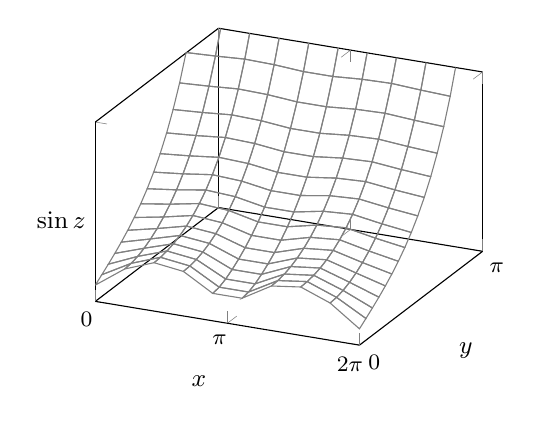
\begin{tikzpicture}
\begin{axis}[small,xlabel={$x$},ylabel={$y$},zlabel={$\abs{\sin z}$},z label style={rotate=-90},colormap={bw}{gray(0 cm)=(0);gray(1 cm)=(1)},zmax=5,xtick={0,180,360},xticklabels={$0$,$\pi$,$2\pi$},ytick={0,180},yticklabels={$0$,$\pi$},ztick=\empty,ymax=180]
\addplot3[mesh,color=gray,domain=0:360,y domain=0:180,samples=10,samples y=20]{sqrt((sin(x)*cosh(pi/180*y))^2+(cos(x)*sinh(pi/180*y))^2)};
\end{axis}
\end{tikzpicture}
\caption{$\sin z$ کی مقیاسی سطح}
\label{شکل_مخلوط_مقیاسی_سطح}
\end{figure}

شکل\حوالہ{شکل_مخلوط_مقیاسی_سطح} میں \عددی{\sin z} کی مقیاسی سطح دکھائی گئی ہے۔مقیاسی سطحیں برقی انجینئری میں بہت کار آمد ثابت ہوتی ہیں۔

%====================
\ابتدا{سوال}\quad
دکھائیں کہ \عددی{\cos z}، \عددی{\sin z}، \عددی{\cosh z} اور \عددی{\sinh z} تمام \عددی{z} کے لئے تحلیلی ہیں۔
\انتہا{سوال}
%====================
\ابتدا{سوال}\quad
مساوات \حوالہ{مساوات_مخلوط_ہذلولی_تعریف_ت} ثابت کریں۔
\انتہا{سوال}
%===================
\ابتدا{سوال}\quad
مساوات \حوالہ{مساوات_مخلوط_ہذلولی_تعریف_الف} سے مساوات \حوالہ{مساوات_مخلوط_ہذلولی_تعریف_ٹ} حاصل کریں۔
\انتہا{سوال}
%======================
\ابتدا{سوال}\quad
مساوات \حوالہ{مساوات_مخلوط_ہذلولی_تعریف_ث} ثابت کریں۔
\انتہا{سوال}
%=====================
\ابتدا{سوال}\quad
مساوات \حوالہ{مساوات_مخلوط_ہذلولی_تعریف_ج} ثابت کریں۔
\انتہا{سوال}
%=====================
\ابتدا{سوال}\quad
مساوات \حوالہ{مساوات_مخلوط_ہذلولی_تعریف_م} ثابت کریں۔
\انتہا{سوال}
%=====================
سوال \حوالہ{سوال_مخلوط_تفاعل_قیمت_الف} تا سوال \حوالہ{سوال_مخلوط_تفاعل_قیمت_ب} میں دی گئی تفاعل کی قیمت دریافت کریں جہاں \عددی{z=x+iy} ہے۔

%===============
\ابتدا{سوال}\شناخت{سوال_مخلوط_تفاعل_قیمت_الف}\quad
$\abs{\cos z}$\\
جواب:\quad
$\sqrt{\cos^2 x+\sinh^2 y}$
\انتہا{سوال}
%=====================
\ابتدا{سوال}\quad
$\abs{\sin z}$\\
جواب:\quad
$\sqrt{\sin^2 x+\sinh^2 y}$
\انتہا{سوال}
%=====================
\ابتدا{سوال}\quad
$\abs{\tan z}$\\
جواب:\quad
$\sqrt{\frac{\sin^2 x+\sinh^2 y}{\cos^2 x+\sinh^2 y}}$
\انتہا{سوال}
%=====================
\ابتدا{سوال}\quad
$\tan z \text{حقیقی}$\\
جواب:\quad
$\tfrac{\sin^2 x+\sinh^2 y}{\sin x\cos x}$
\انتہا{سوال}
%=====================
\ابتدا{سوال}\quad
$\cot z \text{حقیقی}$\\
جواب:\quad
$\tfrac{\sin x\cos x}{\sin^2 x+\sinh^2 y}$
\انتہا{سوال}
%=====================
\ابتدا{سوال}\شناخت{سوال_مخلوط_تفاعل_قیمت_ب}\quad
$\sec z \text{حقیقی}$\\
جواب:\quad
$\tfrac{\cos x\cosh y}{\cos^2 x+\sinh^2 y}$
\انتہا{سوال}
%=====================
سوال \حوالہ{سوال_مخلوط_اعدادی_قیمتیں_حاصل_کریں_الف} تا سوال \حوالہ{سوال_مخلوط_اعدادی_قیمتیں_حاصل_کریں_ب} میں اعدادی قیمتیں حاصل کریں۔

%===============
\ابتدا{سوال}\شناخت{سوال_مخلوط_اعدادی_قیمتیں_حاصل_کریں_الف}\quad
$\sin i$\\
جواب:\quad
$i1.175$
\انتہا{سوال}
%========================
\ابتدا{سوال}\quad
$\sinh i$\\
جواب:\quad
$i0.841$
\انتہا{سوال}
%========================
\ابتدا{سوال}\quad
$\sinh(1+i)$\\
جواب:\quad
$0.635+i1.298$
\انتہا{سوال}
%========================
\ابتدا{سوال}\quad
$\cos(3.2-i5.3)$\\
جواب:\quad
$-100-i5.847$
\انتہا{سوال}
%========================
\ابتدا{سوال}\شناخت{سوال_مخلوط_اعدادی_قیمتیں_حاصل_کریں_ب}\quad
$\cosh(-2-i3)$\\
جواب:\quad
$-3.725+i0.512$
\انتہا{سوال}
%========================
سوال \حوالہ{سوال_مخلوط_تلاش_تمام_حل_الف} تا سوال \حوالہ{سوال_مخلوط_تلاش_تمام_حل_ب} میں دی گئی مساوات کے تمام حل تلاش کریں۔

%===========
\ابتدا{سوال}\شناخت{سوال_مخلوط_تلاش_تمام_حل_الف}\quad
$\cos z=5$\\
جواب:\quad
$\mp2n\pi\mp i2.29,\quad n=0,1,\cdots$
\انتہا{سوال}
%===================
\ابتدا{سوال}\quad
$\sin z=10$\\
جواب:\quad
$\mp 2n\pi- i2.99,\quad n=0,1,\cdots$
\انتہا{سوال}
%===================
\ابتدا{سوال}\quad
$\cosh z=0$\\
جواب:\quad
$\mp i (2n+1)\frac{\pi}{2}, \quad n=0,1,\cdots$
\انتہا{سوال}
%===================
\ابتدا{سوال}\quad
$\cosh z=0.5$\\
جواب:\quad
$\mp i 2n \pi\mp i\frac{\pi}{3}, \quad n=0,1,\cdots$
\انتہا{سوال}
%===================
\ابتدا{سوال}\quad
$\sinh z=0$\\
جواب:\quad
$\mp i n \pi, \quad n=0,1,\cdots$
\انتہا{سوال}
%===================
\ابتدا{سوال}\شناخت{سوال_مخلوط_تلاش_تمام_حل_ب}\quad
$\sin z=i\sinh 1$\\
جواب:\quad
$i\mp 2n\pi$
\انتہا{سوال}
%===================
سوال \حوالہ{سوال_مخلوط_تصدیق_تعلق_الف} تا سوال \حوالہ{سوال_مخلوط_تصدیق_تعلق_ب} میں دیے تعلق کی تصدیق کریں۔

%================
\ابتدا{سوال}\شناخت{سوال_مخلوط_تصدیق_تعلق_الف}\quad
$\cos z=\cosh iz,\quad \sin z=-i\sinh z$
\انتہا{سوال}
%======================
\ابتدا{سوال}\quad
$(\cosh z)'=\sinh z,\quad (\sinh z)'=\cosh z$
\انتہا{سوال}
%======================
\ابتدا{سوال}\quad
\begin{align*}
\cosh z&=\cosh x\cos y+i\sinh x\sin y,\\ 
\sinh z&=\sinh x\cos y+i\cosh x\sin y
\end{align*}
\انتہا{سوال}
%======================
\ابتدا{سوال}\quad
$\abs{\sinh y}\le \abs{\sin z}\le \cosh y,\quad \abs{\sinh y}\le \abs{\cos z}\le \cosh y$
\انتہا{سوال}
%================
\ابتدا{سوال}\quad
$\cosh^2 z-\sinh^2=1$
\انتہا{سوال}
%====================
\ابتدا{سوال}\quad تمام \عددی{z} کے لئے 
$\cot z \ne \mp i$
\انتہا{سوال}
%======================
\ابتدا{سوال}\quad \عددی{\tanh z} کا دوری عرصہ \عددی{i\pi} ہے۔
\انتہا{سوال}
%===========================
\ابتدا{سوال}\quad
\عددی{\cos z=0} صرف حقیقی \عددی{z} کے لئے ہے۔
\انتہا{سوال}
%=================
\ابتدا{سوال}\شناخت{سوال_مخلوط_تصدیق_تعلق_ب}\quad
\عددی{\sin z=0} صرف حقیقی \عددی{z} کے لئے ہے۔
\انتہا{سوال}
%=================
\ابتدا{سوال}\quad
مساوات \حوالہ{مساوات_مخلوط_ہذلولی_تعریف_الف} استعمال کرتے ہوئے درج ذیل ثابت کریں۔\\
$\cos^4 \theta=\frac{1}{8}(\cos 4\theta+4\cos 2\theta+3)$
\انتہا{سوال}
%==================
\ابتدا{سوال}\quad 
مساوات \حوالہ{مساوات_مخلوط_قوت_نمائی_تعریف_ٹ} اور \عددی{1+z+z^2+\cdots=\tfrac{1}{1-z},\quad z=e^{i\tfrac{\theta}{2}}} استعمال کرتے ہوئے درج ذیل ثابت کریں۔
\begin{align*}
1+\tfrac{1}{2}\cos \theta+\tfrac{1}{4}\cos 2\theta+\tfrac{1}{8}\cos 3\theta+\cdots=\frac{4-2\cos \theta}{5-4\cos \theta}
\end{align*}
\انتہا{سوال}
%===================

\حصہ{لوگارتھم۔ عمومی طاقت}\شناخت{حصہ_تحلیلی_لوگارتھم_عمومی_طاقت}
\عددی{z} کی \ترچھا{قدرتی لوگارتھم}\اصطلاح{لوگارتھم!قدرتی}\حاشیہب{natural logarithm}\فرہنگ{logarithm!natural} کو \عددی{\ln z} (بعض اوقات \عددی{\log z}) سے ظاہر کیا جاتا ہے۔قوت نمائی تفاعل کی الٹ کو قدرتی لوگارتھم کہتے ہیں (یہ قدرتی لوگارتھم کی تعریف ہے) یوں ہر \عددی{z\ne 0} کے کئے  \عددی{w=\ln z} کی تعریف درج ذیل تعلق ہے۔
\begin{align}\label{مساوات_مخلوط_لوگارتھم_الف}
e^w=z
\end{align}

مساوات \حوالہ{مساوات_مخلوط_لوگارتھم_الف} میں \عددی{w=u+iv} اور \عددی{z=\abs{z}e^{i\theta}=re^{i\theta}} پر کرتے ہوئے
\begin{align*}
e^w=e^{u+iv}=e^ue^{iv}=re^{i\theta}
\end{align*}
ملتا ہے۔ مساوات کی دونوں اطراف حتمی قیمت یکساں ہو گی۔مساوات \حوالہ{مساوات_مخلوط_خیالی-قوت_نمائی_حتمی_اکائی} کے تحت \عددی{\abs{e^{iv}}=1} ہے لہٰذا  \عددی{e^ue^{i\theta}} کی حتمی قیمت \عددی{e^u} ہو گی۔اسی طرح \عددی{re^{i\theta}} کی حتمی قیمت \عددی{r} ہے لہٰذا
\begin{align*}
e^u=\abs{z}=r \quad \implies \quad u=\ln \abs{z}
\end{align*}
لکھا جا سکتا ہے جہاں \عددی{\ln \abs{z}} مثبت عدد \عددی{\abs{z}} کی بنیادی حقیقی قدرتی لوگارتھم  ہے۔اسی طرح مساوات کی دونوں اطراف دلیل بھی یکساں ہو گی:
\begin{align*}
v=\theta=z\,\text{دلیل}
\end{align*}
یوں درج ذیل ہو گا۔
\begin{align}\label{مساوات_مخلوط_لوگارتھم_ب}
\ln z=\ln\abs{z}+i(z\,\text{دلیل})=\ln\sqrt{x^2+y^2}+i (z\,\text{دلیل})
\end{align}
چونکہ مخلوط \عددی{z} کی دلیل ہر \عددی{2n\pi} پر دہراتا ہے لہٰذا مخلوط قدرتی لوگارتھم کی لامتناہی قیمتیں ہوں گی۔

دلیل \عددی{z} کی صدر قیمت
\begin{align*}
-\pi<z\,\text{دلیل}\le \pi\quad \quad \quad \text{\RL{(حصہ \حوالہ{حصہ_مخلوط_قطبی_صورت_عدم_مساوات})}}
\end{align*}
پر \عددی{\ln z} کی قیمت کو \عددی{\ln z} کی \اصطلاح{صدر قیمت}\فرہنگ{صدر قیمت}\حاشیہب{principal value}\فرہنگ{principal!value} کہتے ہیں جس کو عموماً \عددی{\Ln z} سے ظاہر کیا جاتا ہے۔

ظاہر ہے کہ \عددی{\ln z} کی باقی قیمتیں درج ذیل ہوں گی
\begin{align}\label{مساوات_مخلوط_لوگارتھم_پ}
\ln z=\Ln z\mp i2n\pi\quad\quad\quad (n=1,2,\cdots)
\end{align}
جن کی خیالی اجزاء میں  \عددی{2\pi} کی مضرب کا فرق پایا جائے گا جو اس حقیقت کے عین مطابق ہے کہ \عددی{e^z} دوری تفاعل ہے جس کا خیالی دوری عرصہ \عددی{i2\pi} ہے۔

مزید حقیقی مثبت  \عددی{z} کی صورت میں \عددی{z\,\text{دلیل}} کی صدر قیمت صفر ہو گی لہٰذا \عددی{\Ln z} کی صدر قیمت اور حقیقی قدرتی لوگارتھم کی قیمت یکساں ہوں گی۔ اگر \عددی{z} حقیقی منفی ہو تب \عددی{z\,\text{دلیل}} کی صدر قیمت \عددی{\pi} ہو گی اور تب درج ذیل ہو گا۔
\begin{align*}
\Ln z=\ln \abs{z}+i\pi
\end{align*}

%=======================
\ابتدا{مثال}\quad \موٹا{قدرتی لوگارتھم۔ صدر قیمت}\\
\begin{align*}
\ln(-1)=\mp i\pi,\mp i3\pi,\mp i5\pi,\cdots, \quad \Ln(-1)=i\pi\\
\ln i=i\frac{\pi}{2},-i\frac{3\pi}{2},i\frac{5\pi}{2},-i\frac{7\pi}{2},i\frac{9\pi}{2},\cdots,\quad \Ln i=i\frac{\pi}{2}\\
\Ln (-i)=-i\frac{\pi}{2},\quad \Ln(-2-i2)=\ln\sqrt{8}-i\frac{3\pi}{4}
\end{align*}
\انتہا{مثال}
%===========================
حقیقی قدرتی لوگارتھم کے قواعد مخلوط قیمتوں کے لئے بھی درست ہیں یعنی
\begin{align}\label{مساوات_مخلوط_لوگارتھم_ت}
\text{(ب)}\quad \ln \frac{z_1}{z_2}=\ln z_1-\ln z_2, \quad \quad \text{(الف)} \quad \ln (z_1z_2)=\ln z_1+\ln z_2
\end{align}
لیکن ان تعلق کا مطلب کچھ یوں لینا ہو گا کہ مساوات کی ایک ہاتھ کی ہر ایک قیمت دوسری ہاتھ کی قیمتوں میں شامل ہے۔ 

%===================
\ابتدا{مثال}\quad \موٹا{مخلوط قیمتوں کی صورت میں مساوات \حوالہ{مساوات_مخلوط_لوگارتھم_ت} کا اطلاق}\\
مان لیں کہ
\begin{align*}
z_1=z_2=e^{i\pi}=-1
\end{align*}
ہے۔اگر ہم
\begin{align*}
\ln z_1=\ln z_2=i\pi
\end{align*}
لیں تب مساوات \حوالہ{مساوات_مخلوط_لوگارتھم_ت} اس صورت درست ہو گی جب ہم \عددی{\ln (z_1z_2)=\ln 1=i2\pi} لکھیں جبکہ صدر قیمت کے لئے یہ  درست نہیں ہے یعنی  \عددی{\Ln(z_1z_2)=\Ln(1)=0}
\انتہا{مثال}
%=========================

مساوات \حوالہ{مساوات_مخلوط_کوشی_ریمان_ثبوت_پ} کو مساوات \حوالہ{مساوات_مخلوط_لوگارتھم_ب} پر لاگو کرتے ہوئے 
\begin{align*}
\frac{\dif}{\dif z}\ln z&=\frac{\partial}{\partial x}\ln\sqrt{x^2+y^2}+i\frac{\partial}{\partial x}(z\,\text{دلیل})\\
&=\frac{x}{x^2+y^2}+i\frac{1}{1+\big(\frac{y}{x}\big)^2}\big(-\frac{y}{x^2}\big)=\frac{x-iy}{x^2+y^2}=\frac{1}{z}
\end{align*}
ملتا ہے۔اس طرح قدرتی لوگارتھم کی تفرق درج ذیل ہے۔
\begin{align}\label{مساوات_مخلوط_لوگارتھم_ٹ}
\frac{\dif}{\dif z}\ln z=\frac{1}{z}\quad \quad \quad (z\ne 0)
\end{align}
یوں صدر قیمت \عددی{\Ln z \, (z\ne 0)} جو واحد قیمتی ہے اور یوں تفاعل کی عمومی تعریف پر پورا اترتا ہے، دائرہ کار \عددی{-\pi<z\,\text{دلیل}<\pi} یعنی ماسوائے منفی حقیقی محور  کے، تمام مخلوط سطح پر تحلیلی ہے۔منفی حقیقی محور پر یہ تفاعل غیر استمراری ہے جہاں اس میں \عددی{2\pi} کی چھلانگ پائی جاتی ہے۔

\موٹا{عمومی طاقت}: مخلوط عدد \عددی{z=x+iy (\ne 0)} کی عمومی طاقت کی تعریف درج ذیل کلیہ ہے۔
\begin{align}\label{مساوات_مخلوط_لوگارتھم_ث}
z^c=e^{c\ln z}\quad \quad \quad (z\ne 0, \quad \text{\RL{مخلوط $c$}})
\end{align}
چونکہ \عددی{\ln z} کی لامتناہی قیمتیں ہیں لہٰذا \عددی{z^c} بھی عموماً کثیر قیمتی ہو گا۔اس کی مخصوص قیمت
\begin{align*}
z^c=e^{c\Ln z}
\end{align*}
کو \عددی{z^c} کی \ترچھا{صدر قیمت}\فرہنگ{صدر!قیمت}\فرہنگ{principal!value} کہتے ہیں۔

\عددی{c=n=1,2,\cdots} کی صورت میں \عددی{z^n} واحد قیمتی ہو گا جس کی وہی قیمت ہو گی جو  \عددی{z} کی عمومی \عددی{n} ویں طاقت کی ہوتی ہے۔اسی طرح \عددی{c=-1,-2,\cdots} کے لئے بھی ایسا ہی ہو گا۔

اگر \عددی{c=\tfrac{1}{n}} ہو جہاں \عددی{n=2,3,\cdots} ہے تب
\begin{align*}
z^c=\sqrt[\leftroot{-2}\uproot{2}n]{z}=e^{(1/n)\ln z}\quad \quad \quad (z\ne 0)
\end{align*}
ہو گا جہاں طاقت (\عددی{1/n\ln z}) کی قیمت \عددی{\tfrac{i2\pi}{n}} کی مضرب تک تعین کی جا سکتی ہے جس سے ہمیں جذر کی \عددی{n} منفرد قیمتیں حاصل ہوں گی، جو حصہ \حوالہ{حصہ_مخلوط_ناطق_تفاعل_جذر} میں حاصل کردہ نتیجہ کے عین مطابق ہے۔ اگر \عددی{c=\tfrac{p}{q}} دو مثبت عدد صحیح کا حاصل تقسیم ہو تب بھی صورت حال یہی ہو گی اور \عددی{z^c} کی محدود تعداد کی منفرد قیمتیں ہوں گی۔البتہ، اگر \عددی{c} حقیقی غیر ناطق یا واقعتاً مخلوط ہو تب \عددی{z^c} کی لامتناہی تعداد کی قیمتیں ہوں گی۔ 

%===============
\ابتدا{مثال}\quad \موٹا{عمومی طاقت}\\
\begin{align*}
i^i=e^{i\ln i}=e^{i[i\tfrac{\pi}{2}\mp i2n\pi]}=e^{-\tfrac{\pi}{2}\pm 2n\pi}
\end{align*}
یہ تمام قیمتیں حقیقی ہیں اور صدر قیمت \عددی{(n=0)} کو درج بالا سے \عددی{e^{-\tfrac{\pi}{2}}} لکھا جا سکتا ہے۔
\انتہا{مثال}
%=====================

روایتی طور پر حقیقی مثبت \عددی{z=x} کی صورت میں \عددی{z^c} کا مطلب \عددی{e^{c\ln x}} لیا جاتا ہے جہاں \عددی{\ln x} بنیادی حقیقی قدرتی لوگارتھم ہے (یعنی ہماری تعریف کی رو سے  \عددی{\ln z\,(z=x>0)} کی صدر قیمت)۔اس کے علاوہ اگر \عددی{z=e} (یعنی قدرتی لوگارتھم کی اساس) ہو تب \عددی{z^c=e^c} سے مراد مساوات \حوالہ{مساوات_مخلوط_قوت_نمائی_تعریف_الف} سے حاصل کردہ یکتا قیمت لی جاتی ہے۔

مساوات \حوالہ{مساوات_مخلوط_لوگارتھم_ٹ} سے کسی بھی مخلوط عدد \عددی{a} کے لئے درج ذیل لکھا جا سکتا ہے۔
\begin{align}\label{مساوات_مخلوط_لوگارتھم_ج}
a^z=e^{z\ln a}
\end{align}

%====================
\حصہء{سوالات}

%==============
\ابتدا{سوال}\quad
مساوات \حوالہ{مساوات_مخلوط_لوگارتھم_ت} کی تصدیق \عددی{z_1=i} اور \عددی{z_2=-1} کے لئے  کریں۔
\انتہا{سوال}
%====================
\ابتدا{سوال}\quad
مساوات \حوالہ{مساوات_مخلوط_کوشی_ریمان_قطبی_روپ} استعمال کرتے ہوئے دکھائیں کہ \عددی{\Ln z\,(z\ne 0)} خطہ \عددی{-\pi < \theta<\pi} میں تحلیلی ہے جہاں دلیل \عددی{z} کے زاویہ کی صدر قیمت \عددی{\theta} ہے۔
\انتہا{سوال}
%=====================
\ابتدا{سوال}\quad
دکھائیں کہ منفی حقیقی محور پر \عددی{\Ln z} غیر استمراری ہے۔
\انتہا{سوال}
%=====================
\ابتدا{سوال}\quad
دکھائیں:
$e^{\ln z}=z, \,\ln (e^z)=z\mp i2n\pi,\, n=0,1,\cdots$
\انتہا{سوال}
%======================
سوال \حوالہ{سوال_مخلوط_قیمتیں-_دکھائیں_الف} تا سوال \حوالہ{سوال_مخلوط_قیمتیں-_دکھائیں_ب} میں تمام قیمتیں دریافت کریں۔چند قیمتوں کو مخلوط سطح پر دکھائیں۔

%==============
\ابتدا{سوال}\شناخت{سوال_مخلوط_قیمتیں-_دکھائیں_الف}\quad
$\ln 1$\\
جواب:\quad
$\mp i2n\pi,\quad n=0,1,\cdots$
\انتہا{سوال}
%===================
\ابتدا{سوال}\quad
$\ln 2$\\
جواب:\quad
$0.693\mp i2n\pi,\quad n=0,1,\cdots$
\انتہا{سوال}
%===================
\ابتدا{سوال}\quad
$\ln i$\\
جواب:\quad
$i(\tfrac{\pi}{2}\mp 2n\pi),\quad n=0,1,\cdots$
\انتہا{سوال}
%===================
\ابتدا{سوال}\quad
$\ln e$\\
جواب:\quad
$1\mp i2n\pi,\quad n=0,1,\cdots$
\انتہا{سوال}
%===================
\ابتدا{سوال}\quad
$\ln (ie)$\\
جواب:\quad
$1+i\tfrac{\pi}{2}\mp i2n\pi,\quad n=0,1,\cdots$
\انتہا{سوال}
%===================
\ابتدا{سوال}\quad
$\ln (-ie)$\\
جواب:\quad
$1-i\tfrac{\pi}{2}\mp i2n\pi,\quad n=0,1,\cdots$
\انتہا{سوال}
%===================
\ابتدا{سوال}\quad
$\ln (e^i)$\\
جواب:\quad
$i\mp i2n\pi,\quad n=0,1,\cdots$
\انتہا{سوال}
%===================
\ابتدا{سوال}\شناخت{سوال_مخلوط_قیمتیں-_دکھائیں_ب}\quad
$\ln (e^{-3})$\\
جواب:\quad
$-3\mp i2n\pi,\quad n=0,1,\cdots$
\انتہا{سوال}
%===================
سوال \حوالہ{سوال_مخلوط_لوگارتھم_حل_کریں_الف} تا سوال \حوالہ{سوال_مخلوط_لوگارتھم_حل_کریں_ب} کو \عددی{z} کے لئے حل کریں۔

%================
\ابتدا{سوال}\شناخت{سوال_مخلوط_لوگارتھم_حل_کریں_الف}\quad
$\ln z=-i\tfrac{\pi}{2}$\\
جواب:\quad
$z=-i$
\انتہا{سوال}
%========================
\ابتدا{سوال}\quad
$\ln z=i\tfrac{\pi}{2}$\\
جواب:\quad
$z=i$
\انتہا{سوال}
%========================
\ابتدا{سوال}\quad
$\ln z=1+i\pi$\\
جواب:\quad
$z=-e$
\انتہا{سوال}
%========================
\ابتدا{سوال}\شناخت{سوال_مخلوط_لوگارتھم_حل_کریں_ب}\quad
$\ln z=(1+i)\pi$\\
جواب:\quad
$z=e^{-\pi}$
\انتہا{سوال}
%========================
سوال \حوالہ{سوال_مخلوط_صدر_قیمت_لوگارتھم_الف} تا سوال \حوالہ{سوال_مخلوط_صدر_قیمت_لوگارتھم_ب} میں صدر قیمت  \عددی{\Ln z} دریافت کریں جہاں \عددی{z} دیا گیا ہے۔ 

%================
\ابتدا{سوال}\شناخت{سوال_مخلوط_صدر_قیمت_لوگارتھم_الف}\quad 
$(1-i)^2$\\
جواب:\quad
$0.693-i1.571$
\انتہا{سوال}
%===================
\ابتدا{سوال}\quad 
$\sqrt{2}+i\sqrt{2}$\\
جواب:\quad
$0.693+i0.785$
\انتہا{سوال}
%===================
\ابتدا{سوال}\quad 
$-5$\\
جواب:\quad
$1.609+i\pi$
\انتہا{سوال}
%===================
\ابتدا{سوال}\شناخت{سوال_مخلوط_صدر_قیمت_لوگارتھم_ب}\quad 
$3+i\sqrt{11}$\\
جواب:\quad
$1.498+i0.835$
\انتہا{سوال}
%===================
سوال \حوالہ{سوال_مخلوط_صدر_قیمت_تلاش_الف} تا سوال \حوالہ{سوال_مخلوط_صدر_قیمت_تلاش_ب} میں صدر قیمت دریافت کریں۔

%===============
\ابتدا{سوال}\شناخت{سوال_مخلوط_صدر_قیمت_تلاش_الف}\quad
$(2i)^{\tfrac{1}{2}}$\\
جواب:\quad
$1+i$
\انتہا{سوال}
%==================
\ابتدا{سوال}\quad
$(1+i)^i$\\
جواب:\quad
$0.429+i0.155$
\انتہا{سوال}
%==================
\ابتدا{سوال}\quad
$(1+i)^{1-i}$\\
جواب:\quad
$2.808+i1.318$
\انتہا{سوال}
%==================
\ابتدا{سوال}\quad
$3^{3-i}$\\
جواب:\quad
$12.28-i24.046$
\انتہا{سوال}
%==================
\ابتدا{سوال}\quad
$2^(i2)$\\
جواب:\quad
$0.183+i0.983$
\انتہا{سوال}
%==================
\ابتدا{سوال}\quad
$(2-i)^{1+i}$\\
جواب:\quad
$3.35+i1.189$
\انتہا{سوال}
%==================
\ابتدا{سوال}\شناخت{سوال_مخلوط_صدر_قیمت_تلاش_ب}\quad
$(2+i)^{3-i2}$\\
جواب:\quad
$27.588-i6.126$
\انتہا{سوال}
%==================
الٹ سائن یعنی \عددی{w=\sin^{-1} z} سے مراد (کی تعریف) ایسا تفاعل ہے جو \عددی{\sin w=z} کی تعلق کو مطمئن کرتا ہو۔اسی طرح الٹ کوسائن \عددی{w=\cos^{-1}z} سے مراد ایسا تفاعل ہے جو \عددی{\cos w=z} کو مطمئن کرتا ہو۔باقی تمام الٹ تکونیاتی تفاعل اور الٹ ہذلولی تکونیاتی تفاعل کی تعریف بھی اسی طرح کی جاتی ہے۔طاقتی روپ (مثلاً \عددی{\sin w=(e^{iw}-e^{-iw})/i2} وغیرہ) استعمال کرتے ہوئے سوال \حوالہ{سوال_مخلوط_تعلق_درکار_الف} تا سوال \حوالہ{سوال_مخلوط_تعلق_درکار_ب} میں دیے گئے تعلق کی تصدیق کریں۔

%===========
\ابتدا{سوال}\شناخت{سوال_مخلوط_تعلق_درکار_الف}\quad
$\sin^{-1}z=-i\ln(iz+\sqrt{1-z^2})$
\انتہا{سوال}
%==================
\ابتدا{سوال}\quad
$\cos^{-1}z=-i\ln(z+\sqrt{z^2-1})$
\انتہا{سوال}
%==================
\ابتدا{سوال}\quad
$\cosh^{-1}z=\ln(z+\sqrt{z^2-1})$\\
جواب:
\begin{align*}
\cosh w=\frac{e^w+e^{-w}}{2}=z,\quad \frac{e^{2w}+1}{2e^{w}}=z,\quad e^{2w}-2ze^{w}+1=0\\
e^w=z+\sqrt{z^2-1},\quad w=\ln (z+\sqrt{z^2-1})
\end{align*}
\انتہا{سوال}
%==================
\ابتدا{سوال}\quad
$\sinh^{-1}z=\ln(z+\sqrt{z^2+1})$
\انتہا{سوال}
%==================
\ابتدا{سوال}\quad
$\tan^{-1}z=\frac{i}{2}\ln\frac{i+z}{i-z}$
\انتہا{سوال}
%==================
\ابتدا{سوال}\شناخت{سوال_مخلوط_تعلق_درکار_ب}\quad
$\tanh^{-1}z=\frac{1}{2}\ln\frac{1+z}{1-z}$
\انتہا{سوال}
%==================
\ابتدا{سوال}\شناخت{سوال_تحلیلی_صدر_قیمت_الٹ_سائن_تفاعل}\quad
دکھائیں کہ \عددی{w=\sin^{-1}z} کثیر قیمتی ہے، اور اگر \عددی{w_1} ان میں سے ایک ہو تب باقی کی روپ \عددی{w_1\mp2n\pi} اور \عددی{\pi-w_1\mp2n\pi} ہو گی جہاں \عددی{n=0,1,\cdots} ہے۔\\
(\عددی{w=u+iv=\sin^{-1}z} کی صدر قیمت سے مراد (کی تعریف) وہ قیمت ہے جس کا \عددی{v\ge 0} کی صورت میں \عددی{-\tfrac{\pi}{2}\le y\le \tfrac{\pi}{2}} ہو اور \عددی{v<0} کی صورت میں \عددی{-\tfrac{\pi}{2}<u<\tfrac{\pi}{2}} ہو۔)\\
جواب:\quad
\عددی{\sin(w\mp2n\pi)=\sin w} اور \عددی{\sin(\pi-w)=\sin w} سے یک دم یہ نتیجہ اخذ ہوتا ہے۔
\انتہا{سوال}
%======================
